%% 
%% Copyright 2019-2020 Elsevier Ltd
%% 
%% This file is part of the 'CAS Bundle'
%% --------------------------------------
%% 
%% It may be distributed under the conditions of the LaTeX Project Public
%% License, either version 1.2 of this license or (at your option) any
%% later version.  The latest version of this license is in
%%    http://www.latex-project.org/lppl.txt
%% and version 1.2 or later is part of all distributions of LaTeX
%% version 1999/12/01 or later.
%% 
%% The list of all files belonging to the 'CAS Bundle' is
%% given in the file `manifest.txt'.
%% 
%% Template article for cas-sc documentclass for 
%% double column output.

%\documentclass[a4paper,fleqn,longmktitle]{cas-sc}
\documentclass[a4paper,fleqn,twocolum]{cas-sc}

\usepackage[numbers]{natbib}
% \usepackage[authoryear]{natbib}
% \usepackage[authoryear,longnamesfirst]{natbib}


\usepackage{siunitx}
\usepackage{graphicx}
\usepackage{amsmath} 
\usepackage{makecell}
\usepackage{multirow}
\usepackage{nomencl}
\usepackage{etoolbox}
\usepackage{amsthm}
\usepackage{amsfonts}
\usepackage{mathtools}
\usepackage{textcomp}
\usepackage{caption}
\usepackage{subcaption}
\usepackage{lineno}
\usepackage{multicol}

\usepackage{amssymb}
\usepackage{graphicx}
\usepackage{hyperref}
\usepackage{listings}
\usepackage{soul}

\usepackage{mathrsfs}  
\usepackage{esvect}
\usepackage{amsfonts}
\usepackage{cleveref}
\usepackage{placeins}

\usepackage{tikz}
\usetikzlibrary{
    arrows.meta,
    calc,
    decorations.pathmorphing,
    positioning,
    shapes.geometric
}

\modulolinenumbers[5]

%%%Author definitions
\def\tsc#1{\csdef{#1}{\textsc{\lowercase{#1}}\xspace}}
\tsc{FEM}

% \newcommand{\todo}[1]{\textcolor{red}{(??) #1}}
\newcommand{\todo}[1]{\hl{(??) #1}}
\newcommand{\ignore}[1]{}

\renewcommand*{\figureautorefname}{Fig.}
\renewcommand*{\equationautorefname}{Eq.}
\renewcommand*{\sectionautorefname}{Section}
\renewcommand*{\subsectionautorefname}{Section}
\renewcommand*{\subsubsectionautorefname}{Section}
\newtheorem{proposition}{Proposition}
\newtheorem{remark}{Remark}
\newtheorem{corollary}{Corollary}


\def\Of{\Omega_{\mbox{\scriptsize f}}}
\def\Gf{\Gamma_{\mbox{\scriptsize fs}}}
\def\Gm{\Gamma_{\mbox{s}}}
\def\Gin{\Gamma_{\mbox{\scriptsize in}}}
\def\Gout{\Gamma_{\mbox{\scriptsize out}}}
\def\Gb{\Gamma_{\mbox{\scriptsize b}}}
\def\Gfh{\Gamma_{\mbox{\scriptsize fs,h}}}
\def\Gmh{\Gamma_{\mbox{\scriptsize s,h}}}
\def\Ginh{\Gamma_{\mbox{\scriptsize in,h}}}
\def\Gouth{\Gamma_{\mbox{\scriptsize out,h}}}
\def\Gbh{\Gamma_{\mbox{\scriptsize b,h}}}
\def\Lm{\Lambda_{\mbox{\scriptsize m}}}
\def\Lmh{\Lambda_{\mbox{\scriptsize s,h}}}
\def\V{\mathcal{V}}
\def\Q{\mathcal{Q}}
\def\hatV{\hat{\V}}
\def\VGf{\V_{\Gf}}
\def\VGm{\V_{\Gm}}
\def\uvec{\mathbf{u}}
\def\nvec{\mathbf{n}}
\def\xvec{\mathbf{x}}
\def\qvec{\mathbf{q}}
\def\Ekf{E_{\mbox{\scriptsize kin,flow}}}
\def\Epf{E_{\mbox{\scriptsize pot,flow}}}
\def\Eks{E_{\mbox{\scriptsize kin,str}}}
\def\Ees{E_{\mbox{\scriptsize ela,str}}}
\def\Eeb{E_{\mbox{\scriptsize bend,str}}}
\def\Pds{P_{\mbox{\scriptsize str}}}
\def\Ekr{E_{\mbox{\scriptsize kin,res}}}
\def\Eer{E_{\mbox{\scriptsize ela,res}}}
\def\Pdr{P_{\mbox{\scriptsize res}}}
\def\Et{E_{\mbox{\scriptsize total}}}
\def\Pt{P_{\mbox{\scriptsize total}}}
\def\Eth{E_{\mbox{\scriptsize total,h}}}

\def \utrps{\ensuremath \, \si{\radian \, s^{-1}}}
\def \utm{\ensuremath \, \si{\meter}}
\def \uthertz{\ensuremath \, \si{\hertz}}
\def \utMPa{\ensuremath \, \si{\mega \pascal}}
\def \utMN{\ensuremath \, \si{\mega \newton}}
\def \utPa{\ensuremath \, \si{\pascal}}
\def \utdensity{\ensuremath \, \si{\kilo \gram \per \meter \cubed}}
\def \utkgbym{\ensuremath \, \si{\kilo \gram \per \meter}}
\def \utmsq{\ensuremath \, \si{\meter \squared}}
\def \uin{u_{\text{\scriptsize in}}}
\def \uout{u_{\text{\scriptsize out}}}
\def \thetavec{\boldsymbol{\theta}}



% Uncomment and use as if needed
%\newtheorem{theorem}{Theorem}
%\newtheorem{lemma}[theorem]{Lemma}
%\newdefinition{rmk}{Remark}
%\newproof{pf}{Proof}
%\newproof{pot}{Proof of Theorem \ref{thm}}

\begin{document}
\let\WriteBookmarks\relax
\def\floatpagepagefraction{1}
\def\textpagefraction{.001}

% Short title
\shorttitle{LRMM on floating membrane}

% Short author
\shortauthors{Agarwal, Gómez, Colomés}

% Main title of the paper
\title[mode = title]{Locally resonant hydroelastic structures}                      
% Title footnote mark
% eg: \tnotemark[1]
% \tnotemark[1,2]

% Title footnote 1.
% eg: \tnotetext[1]{Title footnote text}
% \tnotetext[<tnote number>]{<tnote text>} 
% \tnotetext[1]{This document is the results of the research
   % project funded by the Dutch Research Council.}

% \tnotetext[2]{The second title footnote which is a longer text matter
%    to fill through the whole text width and overflow into
%    another line in the footnotes area of the first page.}


% First author
%
% Options: Use if required
% eg: \author[1,3]{Author Name}[type=editor,
%       style=chinese,
%       auid=000,
%       bioid=1,
%       prefix=Sir,
%       orcid=0000-0000-0000-0000,
%       facebook=<facebook id>,
%       twitter=<twitter id>,
%       linkedin=<linkedin id>,
%       gplus=<gplus id>]
\author[1]{Shagun Agarwal}[
    orcid=0000-0003-1922-4242]

% Corresponding author indication
\cormark[1]

% Email id of the first author
\ead{s.agarwal@tudelft.nl}

%  Credit authorship
\credit{Writing - Original Draft, Conceptualization, Methodology, Software, Formal analysis, Investigation, Visualization}


% Second author
\author[1]{Andrei B. Fărăgău}[
    orcid=0000-0001-6397-1961]
    
\ead{a.b.faragau@tudelft.nl}
\credit{Writing - Review \& Editing, Methodology}


% Next author
\author[1]{Oriol Colomés}[
    orcid=0000-0002-5552-9695]
    
\ead{j.o.colomesgene@tudelft.nl}
\credit{Writing - Review \& Editing, Conceptualization, Methodology, Software, Funding acquisition}


% Address/affiliation
\affiliation[1]{organization={Delft University of Technology},
    addressline={Stevinweg 1}, 
    city={Delft},    
    postcode={2628 CN},     
    country={The Netherlands}}


% Corresponding author text
\cortext[cor1]{Corresponding author}

% Footnote text


% Here goes the abstract
\begin{abstract}
Floating flexible plates with attached resonators couple water-wave radiation
to the modes of the host structure and its local oscillators. We formulate
this interaction using a monolithic finite-element model for linear potential
flow coupled to a pre-tensioned plate and discrete mass--spring--damper
resonators. We also derive a local effective-medium dispersion relation for
spatially varying resonator populations. For identical lossless resonators,
the homogeneous relation reduces to a quadratic equation in squared
frequency, which gives two coupled dispersion branches. Deep- and shallow-water
limits and frequency- and density-graded populations are examined, and the
finite-element formulation is used to compute coupled modes of a finite plate.
The effective-medium relation is local and relies on scale separation; it is
not, by itself, a prediction of reflection, transmission, or absorption by a
finite array. The analysis is restricted to linear waves and linear structural
and resonator response.
\end{abstract}

% Use if graphical abstract is present
% \begin{graphicalabstract}
% \includegraphics{figs/grabs.pdf}
% \end{graphicalabstract}

% Research highlights
% \input{skb_highlights}

% Keywords
% Each keyword is seperated by \sep
\begin{keywords}
Monolithic \sep FEM \sep Resonator \sep Floating membrane \sep Hydroelasticity
\end{keywords}


    

\maketitle

\linenumbers

%%%%%%%%%%%%%%%%%%%%%%%%%%%%%%%%%%%%%%%%%%%%%%%%%
%================================================
\section{Introduction}

\begin{itemize}
    {\color{red} \item background, application of vlfs and flexible structures (membranes) for offshore}
The use of very large floating structures (VLFS) in offshore engineering applications is gaining interest in the recent years \cite{lamas2015review}. This interest is mainly driven by the increase of offshore renewable energy technologies, such as wave energy converters \cite{cheng2024wave,renzi2021niche} or floating solar platforms  \cite{liu2024review,huang2023comprehensive}, and floating structures for coastal protection \cite{samuel2025motion,peng2023computational}. Among these, very flexible structures, such as membranes or hinged many-platform, have emerged as a promising solution due to their unique properties, e.g. low mass and potential for deployment over large areas \cite{zhang2022review,koley2022performance}. 
%
Their interaction with waves can be used for wave amplitude attenuation or for energy conversion through
structural and/or added damping \cite{venkateswarlu2021wave,michele2020wave,
collins2021flexible,boren2021distributed,kargar2022atlas,moretti2022high}.

{\color{red}The response of a floating flexible structure depends on the coupling between the fluid, the host structure, and any attached devices. Local resonators
introduce a frequency-dependent impedance and can therefore alter this coupled
response. A local effective-medium dispersion relation describes the response
under scale separation, but by itself it does not establish the scattering
behaviour of a finite structure. In particular, attenuation inferred from a
local complex wavenumber must be distinguished from reflection, transmission,
and absorption calculated for a discrete finite array.

This work formulates a monolithic finite-element model for linear potential
flow coupled to a flexible floating plate and discrete mass--spring--damper
resonators. We derive a local effective-medium dispersion relation for spatially
varying resonator populations and examine homogeneous and graded configurations.
We use the coupled formulation to study modal properties and wave-energy
response, while stating separately the assumptions and scope of the local
dispersion approximation. The analysis is restricted to linear waves and
linear structural and resonator response; nonlinear effects and experimental
validation are outside its scope.}

    {\color{red}\item Explain use of floating membrane as floating breakwaters, wave energy converters or platforms for floating solar or similar applications. Concept of flexibility as key point.}
    Among VLFS, the use of membranes is gaining attention for their benefits in terms of lightweight, reduced cost, easy deployment and serviceability \cite{zhang2022review,koley2022performance}. 
%The key benefit of using flexible membranes is their capacity to attenuate waves by taking advantage of inherent structural damping or added viscous damping when using porous materials, see for example \cite{venkateswarlu2021wave}. Flexible membranes are also being studied for their wave energy harvesting potential, see \cite{michele2020wave,collins2021flexible,boren2021distributed}, converting wave motion to energy through embedded viscoelastic (pietzoelectric or dielectric) power-take-off systems \cite{kargar2022atlas,moretti2022high} or damped mooring systems. The primary advantage of floating viscoelastic membranes (or equivalent flexible structures) lies in their ability to harvest or dissipate energy from a broad range of ocean wave frequencies, leading to increased operational bandwidth and efficiency, as motivated in \cite{agarwal2024dynamic}. %% W-BODY-03 (02 P-02-BIB-01 sec.1, L33): 'as demonstrated in' -> 'as motivated in'.

    {\color{red}
    \item research gap: damping at frequencies outside of natural freqs of the structure}
    Flexible floating structures can be optimized to maximize target quantities of interest, see for example \cite{yao2025optimization,michailides2015optimization}. It has also been recently shown that space-dependent properties of a floating flexible membrane, e.g. mass, can be optimized to maximize wave energy absorption \cite{el4911089optimization}. However, in the viscoelastic membrane of \cite{agarwal2024dynamic} the absorption of wave energy is concentrated in narrow local peaks around the wet natural frequencies of the membrane, since away from them the membrane either heaves almost rigidly (low frequencies) or largely reflects the waves (high frequencies).
%% W-BODY-03 (R-MAP-02 MAJOR-4(d); 02 P-02-BIB-01 sec.1, L37): Agarwal characterisation replaced by 02's verified wording (map B-5: 02 verification).


    %% W-BODY-03 (D-l, D-ac (a); R-MAP-02 MAJOR-4): T-HARV-02 Candidate D, D-now with variant (a), replaces B9 (Candidate A).
    %%   Edits to the 08 text: (1) "A single resonator ... introduces" -> resonator *tuned below* (design condition, MAJOR-4(c));
    %%   (2) "first wet natural frequency" -> "first elastic (non-heave) wet natural frequency" (W-BODY-03b, R-MAP-03 m-N7: was "flexural"): the eq:eigWet heave fixed point
    %%   0.428742-0.273605i (EV-0043, EV-0076) is excluded by name; (3) the 1/2 bound scoped to the two-dimensional particular case
    %%   and a single resonator at the centre of a symmetric membrane (EV-0117, Evans 1976); no 3D analogue given (MAJOR-4(a));
    %%   (4) bandwidth labelled reduced-order (EV-0040, EV-0166: RO 1D zero-draft free-free membrane, no FEM) (MAJOR-4(b));
    %%   (5) Garnaud & Mei re-attributed per 02 P-02-BIB-01 sec.2 ("arrays of small buoys as an alternative to single resonant devices").
    %% TODO-GATED 06 BP-23 (DL-0051) + bare-membrane eq:eigWet fixed-point sweep (R-MAP-02 MAJOR-4 test): confirm which computed root
    %%   is the "first elastic (non-heave) wet natural frequency" of the bare baseline membrane, and that the heave point is correctly excluded.
    %% TODO-GATED D-ad runs (VT-ENERGY-F/VC-02 first; N-1b-H1/H2/H3; RO-ARR-U1/G1; N-ARR-U1/G1; NX-C1 secondary): the closing
    %%   clause "we quantify this in Section~\ref{sec:absorption}" is provisional (D-ac); if the runs fail, fall back to variant (b).
%% W-BODY-03b (R-MAP-03 MAJOR-N1): two-resonator sentence replaced by 12's wording; "unequal damping" is a program reduced-order
%%   result (EV-0113/0147, BP-03) and appears only in subsubsec:absorption_two, labelled reduced-order, until N-1b-H3 passes.
%%   Evans 1976 (two modes each tuned), Merkel 2015 (detuned pair), Jimenez 2017 (asymmetric graded panel) cited for what they show.
%% W-BODY-03b (R-MAP-03 m-N4): closing clause in red until R-H3/R-H4 pass (D-ac); variant (b) fall-back stands.
%%   "identical" arrays: red CITE NEEDED for 02 (candidates per 12: Merkel 2015 N-resonator, Garnaud & Mei 2009); else write "graded" only.
%% W-BODY-03b (R-MAP-03 m-N7): "flexural" -> "elastic (non-heave)" / "elastic": the baseline host is a tensioned membrane, C_rho = 0.
%% W-BODY-04 (R-MAP-03 MAJOR-N1): sentence 4 = 08 T-HARV-02_candidate_D sec.1.1-v2 block verbatim (each source cited for its own
%%   asymmetric route; "narrow bands" scoped to a single pair, not to the Jimenez rainbow panel; Merkel narrow peak per 02 P-02-BIB-02 item 3).
%% W-BODY-04 (R-MAP-03 m-N4): sentence 5 = 08 sec.1.1-v2 drop-"identical" fallback; 02 P-02-BIB-02 item 2: no source for identical arrays.
%%   Garnaud & Mei 2010 is not cited for any entrance-reflection floor (02 item 4). Optional westcott2024broadband (02 item 2) not added: PI/12.
%% W-BODY-05 (D-aq (3), R-BODY-04 m-B2): Evans clause = 12's wording (symmetric and antisymmetric modes, each optimally tuned).
%% W-BODY-05b (D-aq (2)): westcott2024broadband cited next to wilks2022rainbow (02 verified, P-02-BIB-03; graded PTO stiffness, identical buoys).
In this work we propose the integration of damped local resonators into a floating membrane, i.e.\ mass--spring--dashpot units whose dashpot acts as an idealised linear power take-off. A single resonator tuned below the first elastic (non-heave) wet natural frequency of the bare membrane introduces a resonator-dominated wet mode near its own natural frequency. When the resonator damping matches the radiation damping of that mode, the dashpot absorbs incident wave energy at frequencies where the bare membrane has no elastic resonance. In the two-dimensional setting of a vertical section, and for a single resonator at the centre of a symmetric membrane, the absorbed fraction is at most one half, the classical limit for a symmetric absorber radiating to both sides \cite{evans1976theory}; reduced-order models of the membrane give a relative absorption bandwidth of about $2/Q_{\rm rad}$, with $Q_{\rm rad}$ the radiative quality factor of that mode. Two resonators can exceed one half: when the absorber is made asymmetric, absorption of waves incident from one side can approach unity, as for a body whose symmetric and antisymmetric modes of motion are each optimally tuned \cite{evans1976theory}, for a detuned pair of acoustic resonators \cite{merkel2015control} and for asymmetric acoustic panels \cite{jimenez2017rainbow}, although, for a single pair, only within narrow frequency bands. Arrays of resonators graded in natural frequency have been used to extend the working frequency range of acoustic and water-wave absorbers \cite{jimenez2017rainbow,wilks2022rainbow,westcott2024broadband}, and arrays of small buoys have been proposed as an alternative to single resonant wave-energy devices \cite{garnaud2009wave}{\color{red}; for a floating membrane we quantify this in Sections~\ref{subsubsec:num_L2_4} and~\ref{subsec:num_graded} [PROVISIONAL: L2-4 and L2-6 are done; settle the wording in the final pass]}.
    
    {\color{red}\item review of structures with local resonators.}
    
    {\color{red}\item research gap: interaction with hydroelastic structures. There is a need to understand the interaction of these large floating platforms with waves.}
    
    {\color{red}\item objectives of the paper: modeling, assessing performance and parametric study. We are primarily interested in the reflection, transmission and absorption of the wave energy.}

    {\color{red} novelty}
    
    {\color{red}\item organization of the paper.}
\end{itemize}

\input{problem_setting}
\section{Local effective-medium dispersion theory} \label{sec:dispersion_relation}
The effective-medium description of a floating plate carrying distributed resonators was introduced in \cite{liu2025metaplate} and used for graded designs in \cite{liu2025metaplate,jin2026low}. In this section we derive it for a damped, pre-tensioned plate with arbitrary, possibly graded, resonator populations. Then, we use the effective-medium theory to isolate the effect that distinguishes a LHR structure, also denoted by floating metaplate in the literature, from a locally resonant structure in vacuo. In the hydroelastic case, the resonators load the supporting structure, denoted also by host, whose inertia includes the fluid added mass. We will show that the fluid-loaded structure inerta depends on wavenumber and diverges at long wavelength. As a consequence, the effective resonator mass ratio becomes wavenumber dependent (see Section~\ref{subsubsec:fluid_dilution}). This mass ratio sets the strength of the resonator--plate hybridisation and prevents the appearence of a complete stop band of the homogenised floating metaplate.

In this section the local relation is derived by effective-medium homogenization, based on a local spatial density of resonators rather than on a globally repeating unit cell. Let $\boldsymbol{\theta}=(\tilde m,\tilde k,\tilde c)$ denote the density-normalised resonator parameters, i.e mass, stiffness and damping, and let $n(\xvec,\boldsymbol{\theta})$ be their local joint number density, so that $n(\xvec,\boldsymbol{\theta})\,\mathrm{d}\boldsymbol{\theta}$ is the number of resonators per unit plate measure near $\xvec$ whose parameters lie in the subset $\mathrm{d}\boldsymbol{\theta}$. This density may vary with position and may describe anisotropic or graded resonator populations. For a population with common fixed set of parameters, $\boldsymbol{\theta}_r$, it reduces to $n(\xvec,\boldsymbol{\theta})=n(\xvec)\,\delta(\boldsymbol{\theta}-\boldsymbol{\theta}_r)$. 

Let $d_s(\xvec)$ denote a local mean nearest-neighbour spacing and let $L_n(\xvec)=n(\xvec)/\lvert\nabla n(\xvec)\rvert$ denote the characteristic length over which the resonator density changes, with $L_n=\infty$ for a uniform density. The effective-medium approximation applies when the resonator spacing and the scale over which this density varies are small compared with the wavelength, while the physical attachment positions remain arbitrary and need not be periodic. With the local wavelength $\lambda(\xvec)=2\pi/\lvert\mathbf{k}(\xvec)\rvert$, the scale-separation requirements are
\begin{equation}\label{eq:homogenization_scale_separation}
    \varepsilon_s(\xvec)=\frac{d_s(\xvec)}{\lambda(\xvec)}\ll 1,
    \qquad
    \varepsilon_n(\xvec)=\frac{\lambda(\xvec)}{L_n(\xvec)}\ll 1.
\end{equation}
%% [2026-10-28 numerical feedback, J2025-LRMM Sec. 6]
{\color{red}For a line lattice at fixed loading, the finite element results of Section~\ref{subsubsec:num_L1_8} quantify the first condition: the hybridisation of the discrete lattice differs from the local value by a correction of order $\varepsilon_s^{4.5}$, $2.7\times10^{-4}$ at $\varepsilon_s=\tfrac14$ and $6.2\times10^{-7}$ at $\varepsilon_s=\tfrac1{16}$.}

For each discrete resonator, let us define, respectively, the natural frequency and damping ratio as
\begin{equation}\label{eq:resonator_natural_freq_damping}
    \omega_{r,i}^2=\frac{k_{\rho,i}}{m_{\rho,i}},
    \qquad\zeta_i=\frac{c_{\rho,i}}{2\sqrt{k_{\rho,i}m_{\rho,i}}},
    \qquad i=1,\ldots,N.
\end{equation}

Assuming an harmonic motion, from equation \eqref{eq:resonators_freq} we can express the resonator motion amplitude as a function of the plate deflection amplitude at the attachment position, $\eta(\xvec_i)$, as
\begin{equation}\label{eq:resonator_motion}
    q_i(\omega)=\frac{k_{\rho,i}-i\omega c_{\rho,i}}{-\omega^2m_{\rho,i}+k_{\rho,i}-i\omega c_{\rho,i}}\,\eta(\xvec_i),
    \qquad i=1,\ldots,N.
\end{equation}

Using equation \eqref{eq:resonator_motion}, the dynamic force exerted by the $i$-th resonator on the plate can be expressed as
\begin{equation}\label{eq:resonator_force}
    F_i(\omega) = \left(k_{\rho,i}-i\omega c_{\rho,i}\right)\left(q_i-\eta(\xvec_i)\right)=\frac{\omega^2 \,m_{\rho,i}\left(k_{\rho,i}-i\omega c_{\rho,i}\right)}{-\omega^2 m_{\rho,i}+k_{\rho,i}-i\omega c_{\rho,i}}\,\eta(\xvec_i)=\omega^2 \, m_{\mathrm{eff,\rho,i}}(\omega)\,\eta(\xvec_i),
    \qquad i=1,\ldots,N.
\end{equation}
Where $m_{\mathrm{eff,\rho,i}}(\omega)$ is the effective dynamic mass of the $i$-th resonator relative to the fluid density, defined as
\begin{equation}
    m_{\mathrm{eff,\rho,i}}(\omega)=m_{\rho,i}\frac{\left(k_{\rho,i}-i\omega c_{\rho,i}\right)}{-\omega^2 m_{\rho,i}+k_{\rho,i}-i\omega c_{\rho,i}}=m_{\rho,i}\frac{\left(1-2i\zeta_i \frac{\omega}{\omega_{r,i}}\right)}{1-\left(\frac{\omega}{\omega_{r,i}}\right)^2-2i\zeta_i \frac{\omega}{\omega_{r,i}}}.
\end{equation}

Considering the homogenized fluid--structure problem, let $\mathcal{Z}_f(\mathbf{k},\omega)$ denote the local pressure-to-displacement impedance obtained from equation~\eqref{eq:dynamic_bc_m_freq} by taking the fluid Schur complement at a given position $\xvec$:
\begin{equation}\label{eq:fluid_impedance}
    -i\omega\phi\big|_{\Gm}=\mathcal{Z}_f(\mathbf{k},\omega)\eta.
\end{equation}
Here $\mathbf{k}$ is a local wavevector used to probe the homogenized medium, not necessarily a global Bloch wavenumber. The impedance operator is generally complex-valued and may vary with position for general geometries. For a domain with flat bottom of depth $H$ and open boundaries, the local fluid impedance is given by
\begin{equation}\label{eq:Zf_closed_form}
\mathcal Z_f(\mathbf{k},\omega)=\dfrac{-\omega^2}{|\mathbf{k}|\tanh(|\mathbf{k}|H)}.
\end{equation}
In the deep- and shallow-water limits, equation~\eqref{eq:Zf_closed_form} reduces to $\mathcal Z_f\to-\omega^2/|\mathbf{k}|$ for $|\mathbf{k}|H\to\infty$ and to $\mathcal Z_f\to-\omega^2/(|\mathbf{k}|^2H)$ for $|\mathbf{k}|H\to0$, respectively.

\begin{remark}
The dimensionless added mass per unit area, normalized by the fluid density, is
\begin{equation}
    M_{f,\rho}(\mathbf{k},H)
    =
    \frac{1}{|\mathbf{k}|\tanh(|\mathbf{k}|H)},
    \qquad
    \left.
    \frac{\partial M_{f,\rho}}{\partial\omega}
    \right|_{\mathbf{k},H}
    =0.
    \label{eq:plane_wave_added_mass}
\end{equation}
The dimensional added mass per unit area is
$M_f=\rho M_{f,\rho}$. Thus, for the infinite fluid--structure configuration, the hydrodynamic inertia depends on wavenumber and water depth, but not on frequency. The frequency dependence of the
fluid impedance in Eq.~\eqref{eq:Zf_closed_form} enters
through the factor $-\omega^2$, whereas its inertial coefficient is fixed for prescribed $\mathbf{k}$ and $H$.
%
However, for a finite plate, the resulting fluid response depends on frequency through the propagating free-surface wave number, the radiation condition, and the spatial distribution of the structural motion. Eliminating the fluid field by factorization,
therefore, produces a frequency-dependent hydrodynamic operator.
Its inertial and dissipative contributions are commonly interpreted in terms of radiation added mass and radiation damping, respectively.

Therefore, equation \eqref{eq:plane_wave_added_mass} should be understood as a local constitutive result restricted to a uniform medium in an infinite (or periodic) structure. In the finite domain case, the operator and its frequency dependence are instead
determined by the coupled boundary-value problem, as discussed in
Section~\ref{sec:finite_domain}.
\end{remark}

We now use a local plane-wave probe $\eta(\xvec)\propto\exp(i\mathbf{k}\cdot\xvec)$ for the homogenized plate. The pre-tension and bending operators then contribute $T_\rho(1-i\omega\tau)|\mathbf{k}|^2$ and $C_\rho(1-i\omega\tau_b)|\mathbf{k}|^4$, respectively, for an isotropic plate. Replacing the arbitrary point attachments by their local continuous density, following the effective-medium construction of \cite{liu2025metaplate}, gives
\begin{equation}\label{eq:dispersion_relation}
\begin{aligned}
    \mathcal{D}(\mathbf{k},\omega)={}&\mathcal{Z}_f(\mathbf{k},\omega)+g
    +T_\rho(1-i\omega\tau)|\mathbf{k}|^2
    +C_\rho(1-i\omega\tau_b)|\mathbf{k}|^4
    -\omega^2m_{\mathrm{eff},\rho}(\xvec,\omega)=0.
\end{aligned}
\end{equation}
For an anisotropic plate, the bending term in equation~\eqref{eq:dispersion_relation} is replaced by $(\mathbf{C}_\rho(1-i\omega\tau_b):(\mathbf{k}\otimes\mathbf{k})):(\mathbf{k}\otimes\mathbf{k})$. Nonetheless, for the sake of simplicity, we will restrict ourselves to isotropic plates in the following discussion.
The corresponding local effective dynamic mass density is
\begin{equation}\label{eq:effective_mass_dispersion}
    m_{\mathrm{eff},\rho}(\xvec,\omega)
    =m_\rho+\int_{\boldsymbol{\theta}}
    n(\xvec,\boldsymbol{\theta})\,
    \tilde m\,\frac{\tilde k-i\omega \tilde c}
    {\tilde k-\omega^2\tilde m-i\omega \tilde c}
    \,\mathrm{d}\boldsymbol{\theta},
    \qquad \boldsymbol{\theta}=(\tilde m,\tilde k,\tilde c).
\end{equation}
For identical resonators, $n(\xvec,\boldsymbol{\theta})=n(\xvec)\,\delta(\boldsymbol{\theta}-\boldsymbol{\theta}_r)$ with $\boldsymbol{\theta}_r=(m_{\rho,r},k_{\rho,r},c_{\rho,r})$, equation~\eqref{eq:effective_mass_dispersion} reduces to 
\begin{equation}\label{eq:effective_mass_dispersion_single}
  m_{\mathrm{eff},\rho}(\xvec,\omega)=m_\rho+n(\xvec)m_{\rho,r}\frac{k_{\rho,r}-i\omega c_{\rho,r}}{k_{\rho,r}-\omega^2m_{\rho,r}-i\omega c_{\rho,r}}.
\end{equation}
Thus, the effective dispersion relation can vary with $\xvec$ even though the plate material properties are uniform and all the resonators have same properties. Note also that the dispersion relation for uniformly distributed resonators, i.e. $n(\xvec,\thetavec)=n_0$ with $n_0$ a constant density, can still vary with position if the fluid depth is nonuniform, since the fluid impedance $\mathcal{Z}_f(\mathbf{k},\omega)$ depends on the local depth $H(\xvec)$.

In general, both the plate operators and resonator impedances are damped, therefore, the local roots for frequency and wavenumber at a given point $\xvec$, $\omega(\mathbf{k};\xvec)$ or $\mathbf{k}(\omega;\xvec)$, are generally complex-valued. In the non-damped limit, a negative real part of the effective dynamic mass indicates a local dynamic-inertia reversal, but it is not by itself a sufficient criterion for a complete hydroelastic stop band.

\begin{remark}
The relation in equation~\eqref{eq:dispersion_relation} is a local constitutive law, not a global Bloch dispersion relation. To capture the full spatial complexity of the resonator array, the exact arbitrary-position model should be considered, i.e. 
\begin{equation}\label{eq:arbitrary_resonator_distribution}
    \sum_{i=1}^N (k_{\rho,i}-i\omega c_{\rho,i})\left(\eta(\xvec_i)-q_i\right)
    \delta(\xvec-\xvec_i).
\end{equation}
In this regard, the finite element formulation of Section~\ref{sec:numerical_formulation} retains this point distribution and is suitable for such analysis.
\end{remark}

Since the general hydroelastic system involves complex-valued, frequency-dependent variables and a transcendental fluid impedance, numerical root-finding is strictly required. However, by imposing targeted physical assumptions, we can reduce the characteristic equation $\mathcal{D}(\mathbf{k}, \omega) = 0$ to closed-form algebraic expressions that clarify the structure of the local dispersion branches.

\subsection{Non-dissipative homogeneous isotropic LRH plate in flat bottom fluid domain}\label{subsubsec:non-dissipative_homogeneous_isotropic_dispersion}
Let us consider an infinite domain in which the resonators are identical and uniformly distributed, so that $n(\xvec,\boldsymbol{\theta}) = n_0\,\delta(\boldsymbol{\theta}-\boldsymbol{\theta}_r)$ with constant number density $n_0$ (per unit length in 1D, per unit area in 2D) and common resonator parameters $\boldsymbol{\theta}_r=(m_{\rho,r},k_{\rho,r},c_{\rho,r})$. We also assume the non-dissipative limit, i.e. $\tau=0$, $\tau_b=0$, and $c_{\rho,r}=0$. Since the plate is isotropic and the resonator population is spatially uniform, the one- and two-dimensional formulations share the same scalar wavenumber magnitude $k=|\mathbf{k}|$.

Under these assumptions, equation~\eqref{eq:effective_mass_dispersion} reduces to the purely real effective dynamic mass
\begin{equation}
    m_{\mathrm{eff},\rho}(\omega)
    = m_\rho + n_0 m_{\rho,r}\frac{\omega_r^2}{\omega_r^2-\omega^2},
\end{equation}
where $\omega_r = \sqrt{k_{\rho,r}/m_{\rho,r}}$ is the undamped resonator natural frequency. Substituting this expression into the local effective dispersion relation~\eqref{eq:dispersion_relation} gives the homogeneous non-dissipative limit
\begin{equation}
    g + T_\rho k^2 + C_\rho k^4
    - \omega^2\left[m_\rho + n_0 m_{\rho,r}\frac{\omega_r^2}{\omega_r^2-\omega^2} + \frac{1}{k\tanh(kH)}\right]=0,
\end{equation}
which is equivalent to the scalar dispersion law obtained for $\mathcal{Z}_f$ given by equation~\eqref{eq:Zf_closed_form}, with $|\mathbf{k}|=k$. This form is consistent with the previous definitions of $m_{\mathrm{eff},\rho}$, $n_0$, and the fluid impedance, and it remains a local constitutive relation rather than a global Bloch dispersion law.

%% W-BODY-03: B13 applied per D-n (all option a): E-06 L_g, E-07 ka/pi, E-08 s = omega^2, E-19 (E-09/E-10) D-nu and b(k), E-14 Liu mapping.
%% W-BODY-03b (R-MAP-03 m-N12): garbled Liu citation fixed ("in \citep[eqn. 3.4]{...} their equation (3.4)" -> "\citep[eq.~(3.4)]{...}"; "than the" -> "to that").
This simplification leads to a similar effective-plate representation to that derived by Liu et al. \citep[eq.~(3.4)]{liu2025metaplate}, with the only difference being the membrane stiffness term given by the pre-tension $T_\rho$. 
% In the notation of Liu et al., whose groups are dimensional, the parameters of Table~\ref{tab:dispersion_test_parameters} correspond, in SI units and with lattice spacing $a=1/n_0=1~\si{\meter}$, to $\gamma_0=m_\rho=0.01~\si{\meter}$, $\beta=D/(\rho g)=C_\rho/g=0.05~\si{\meter\tothe{4}}$ and $\gamma_1=m_r/(a\rho)=n_0m_{\rho,r}=0.01~\si{\meter}$.
The effect of the resonator population is absorbed into a modified inertial term, resulting into a plate with the same host stiffness but an effective frequency-dependent dynamic mass density. Writing
\begin{equation}
    m_{\mathrm{eq},\rho}(\omega)
    = m_\rho + m_{\mathrm{res},\rho}(\omega),
    \qquad
    m_{\mathrm{res},\rho}(\omega)
    = n_0 m_{\rho,r}\frac{1}{1-\left(\frac{\omega}{\omega_r}\right)^2},
\end{equation}
we obtain the equivalent-plate law
\begin{equation}\label{eq:equivalent_isotropic_plate_dispersion}
    g + T_\rho k^2 + C_\rho k^4
    - \omega^2\left[m_{\mathrm{eq},\rho}(\omega)+\frac{1}{k\tanh(kH)}\right]=0.
\end{equation}

In this simplified setting, the roots of the scalar equation can be interpreted as two dispersion branches separated by the local resonance frequency $\omega_r$, and the two branches anticross around $\omega_r$, bracketing it at every wavenumber. Whether a complete stop band exists must be assessed from the full root structure of the above equation over all wavenumbers, or from a Bloch analysis of the discrete resonator lattice.
%, rather than inferred from the sign of the effective mass or from a finite wavenumber window.
A closed-form solution for the roots of equation~\eqref{eq:equivalent_isotropic_plate_dispersion} is reported in Appendix~\ref{app:closed_form_isotropic}, not presented here for the sake of brevity.

To visualize the dispersion branches for this particular case, let us consider the set of parameters listed in Table~\ref{tab:dispersion_test_parameters}.
%
% This can be removed:
%-------
% The material, geometric and resonator parameters used in the homogeneous and graded dispersion tests, Section~\ref{subsec:graded_resonators}, are shown in Table~\ref{tab:dispersion_test_parameters}. The plate quantities $m_\rho$ and $C_\rho$ are the mass and bending-rigidity parameters appearing in the normalized hydroelastic model. The two pre-tension cases use $T_\rho=0$ and $T_\rho=9.8\ \si{\meter\cubed\per\second\squared}$ ($T=9800\ \si{\newton\per\meter}$), respectively. %% ERRATUM E-03 (PI-approved 2026-10-02; D-d)
% %% E-06 sentence from 04 T-F3-03_slow_grading.md sec.5 (handoff to 13); EV-new (04, eps_n table). L_g = 500a PI-confirmed (D-ah, PI-DECISIONS-2026-10-05).
% %% W-BODY-03b (R-MAP-03 m-N3): PROVISIONAL marker removed (D-ah); "<= 0.10" -> "\lesssim 0.1 (at most 0.104, at omega = 1)" per 04 T-F3-03 sec.2-3.
% We take a slow grading, $L_g=500~\si{\meter}=500a$, for which $\varepsilon_n=\lambda/L_g\lesssim0.1$ (at most $0.104$, at $\omega=1~\si{\radian\per\second}$) for exponential frequency grading and for density grading over the whole plotted band $\omega\in[1,10]~\si{\radian\per\second}$ (both pre-tensions), whereas for linear grading the condition holds only for $\omega\gtrsim2.4$--$2.6~\si{\radian\per\second}$ ($T_\rho=0$ and $T_\rho>0$, respectively) because its local grading length $L_g-x$ vanishes at the low-frequency end.
% ----
%
%
\begin{table}[h!]
    \centering
    \caption{Material, geometric and resonator parameters used in the dispersion tests of Sections~3.1 and~3.2.}
    \label{tab:dispersion_test_parameters}
    \footnotesize
    \begin{tabular}{lll}
        \hline
        Quantity & Symbol & Value \\
        \hline
        Fluid density & $\rho$ & $1000\ \si{\kilogram\per\meter\cubed}$ \\
        Gravity & $g$ & $9.8\ \si{\meter\per\second\squared}$ \\
        Fluid depth & $H$ & $10\ \si{\meter}$ \\
        Plate mass per area & $m_\rho$ & $0.01\ \si{\meter}$ ($m=10\ \si{\kilogram\per\meter\squared}$) \\
        Bending parameter & $C_\rho$ & $0.49\ \si{\meter\tothe{5}\per\second\squared}$ ($D=490\ \si{\newton\meter}$) \\
        Pre-tension & $T_\rho$ & $0$ or $9.8\ \si{\meter\cubed\per\second\squared}$ ($T=9800\ \si{\newton\per\meter}$) \\
        Resonator density & $n_0$ & $1\ \si{\per\meter}$ (1D) \\
        Resonator mass parameter & $m_{\rho,r}$ & $0.01\ \si{\meter\squared}$ (1D) \\
        Resonator frequency & $\omega_r$ & $10\ \si{\radian\per\second}$ \\
        % Grading length & $L_g$ & $500\ \si{\meter}$ ($=500a$) \\
        % Frequency grading range & $\omega_r(x)$ & $10$ to $1\ \si{\radian\per\second}$ \\
        % Density grading law & $n(x)$ & $n_0e^{-x/L_g}$ \\
        \hline
    \end{tabular}
\end{table}
%
%   HEREEE
%
Figure~\ref{fig:subsubsec_non_dissipative_homogeneous_isotropic_dispersion}
shows the explicit dispersion branches for the LRH plate without (left) and with pre-tension (right). In both cases, the lower branch is continuously connected to the bare hydroelastic plate response at frequencies below the local resonance, while the upper branch is predominantly associated with the resonator motion and approaches $\omega_r$ over a broad wavenumber interval. In the figure, the diamonds mark $\omega_\mp(k_c)$, the values of the lower and upper branches $\omega_-(k)$ and $\omega_+(k)$ evaluated at the wavenumber $k_c$, i.e. where the bare-plate branch crosses $\omega_r$. Note that their separation is the anticrossing gap at that crossing point. Since the two branches bracket $\omega_r$ at every wavenumber (Appendix~\ref{app:closed_form_isotropic}), this separation is not, by itself, a stop band of a discrete structure. The parameters of Table~\ref{tab:dispersion_test_parameters} correspond to those of \cite{liu2025metaplate}. With $a=1/n_0$, their crossing wavenumbers, $k_ca/\pi=0.87$ and $0.61$, give $\varepsilon_s=0.44$ and $0.31$ in equation~\eqref{eq:homogenization_scale_separation}, i.e. outside the strict validity range of the local model. We retain them for a direct comparison with \cite{liu2025metaplate}, and Section~\ref{subsubsec:lat_long_wave} uses them to quantify the error of the local model against the exact discrete lattice.

For $T_\rho=0$, the lower branch is governed by the floating plate and fluid inertia, whereas the resonator produces the upper branch and the anticrossing gap marked in Fig.~\ref{fig:subsubsec_non_dissipative_homogeneous_isotropic_dispersion}. Introducing $T_\rho>0$ increases the bare host hydroelastic branch through $T_\rho k^2$, so that it crosses $\omega_r$ at a smaller wavenumber $k_c$, while the resonator frequency $\omega_r$ remains fixed. Since the fluid added mass increases as the wavenumber decreases, pre-tension also reduces the anticrossing gap, from $0.163$ to $0.138$. In Section~\ref{subsubsec:fluid_dilution} we show that this reduction is precisely given by the fluid added mass at $k_c$.
\begin{figure}[pos=htbp]
    \centering
    \includegraphics[width=0.49\linewidth]{figures/LRH_t0.png}
    \hfill
    \includegraphics[width=0.49\linewidth]{figures/LRH_tpositive.png}
    \caption{Explicit local dispersion branches for the non-dissipative homogeneous isotropic LRH plate considering zero pre-tension, $T_\rho=0$ (left), and positive pre-tension, $T_\rho>0$ (right). Diamonds mark $\omega_\mp(k_c)$ at $\pm k_c a/\pi$, where the bare branch crosses $\omega_r$ (anticrossing gap $(\omega_+-\omega_-)/\omega_r=\sqrt{\mu(k_c)}=0.163$ for $T_\rho=0$ and $0.138$ for $T_\rho>0$, equation~\eqref{eq:anticrossing}).}
    \label{fig:subsubsec_non_dissipative_homogeneous_isotropic_dispersion}
\end{figure}

{\color{red} %To review
\subsubsection{Fluid dilution of the resonator mass ratio}\label{subsubsec:fluid_dilution}
Dividing the quadratic form of equation~\eqref{eq:equivalent_isotropic_plate_dispersion} (Appendix~\ref{app:closed_form_isotropic}) by the total host inertia, $m_\rho+M_{f,\rho}(k,H)$, shows that the coupling between plate and resonators is controlled by two quantities only. The first is the bare hydroelastic branch, $\omega_0^2(k)=K(k)/\big(m_\rho+M_{f,\rho}(k,H)\big)$, with $K(k)=g+T_\rho k^2+C_\rho k^4$. The second is the wavenumber-dependent mass ratio
\begin{equation}\label{eq:lat_mu}
    \mu(k)=\frac{n_0\,m_{\rho,r}}{m_\rho+M_{f,\rho}(k,H)} .
\end{equation}
Indeed, with $s=\omega^2$, the homogeneous non-dissipative dispersion relation reads
\begin{equation}\label{eq:normalised_quadratic}
    s^2-\big[\omega_0^2(k)+\omega_r^2\big(1+\mu(k)\big)\big]s+\omega_0^2(k)\,\omega_r^2=0 .
\end{equation}
In vacuo, $M_{f,\rho}=0$ and $\mu=n_0m_{\rho,r}/m_\rho$ is a constant fixed by the design: it is the mass ratio that sets the local-resonance gap $[\omega_r,\omega_r\sqrt{1+\mu}]$ of a metaplate \cite{xiao2012flexural}. For a floating plate, the fluid added mass enters the denominator of equation~\eqref{eq:lat_mu} and dilutes the resonators. This has two consequences.

\paragraph{Hybridisation strength.} At the crossing wavenumber $k_c$, defined by $\omega_0(k_c)=\omega_r$, the roots of equation~\eqref{eq:normalised_quadratic} satisfy $s_+s_-=\omega_r^4$ and $s_++s_-=\omega_r^2\big(2+\mu(k_c)\big)$. Hence $(\omega_+-\omega_-)^2=s_++s_--2\sqrt{s_+s_-}=\mu(k_c)\,\omega_r^2$, that is,
\begin{equation}\label{eq:anticrossing}
    \frac{\omega_+(k_c)-\omega_-(k_c)}{\omega_r}=\sqrt{\mu(k_c)} ,
\end{equation}
exactly within the local model. For the parameters of Table~\ref{tab:dispersion_test_parameters}, the plate-only mass ratio is $n_0m_{\rho,r}/m_\rho=1$. The added mass at the crossing, however, is $M_{f,\rho}(k_c,H)=0.365$~m for $T_\rho=0$ and $0.519$~m for $T_\rho>0$. Hence $\mu(k_c)=0.0267$ and $0.0189$, and equation~\eqref{eq:anticrossing} gives the gaps $0.163$ and $0.138$ of Figure~\ref{fig:subsubsec_non_dissipative_homogeneous_isotropic_dispersion}. Relative to the same structure in vacuo, the fluid reduces the hybridisation by the factor $\sqrt{m_\rho/(m_\rho+M_{f,\rho}(k_c,H))}$, i.e. by about $6$ and $7$, respectively. Pre-tension raises $\omega_0(k)$, lowers $k_c$ and increases $M_{f,\rho}(k_c,H)$; at fixed resonator mass, it therefore weakens the hybridisation. In deep water and for $M_{f,\rho}\gg m_\rho$, $M_{f,\rho}\simeq1/k_c$, and equation~\eqref{eq:anticrossing} gives the design rule
\begin{equation}\label{eq:dilution_design_rule}
    n_0\,m_{\rho,r}\simeq\Big(\frac{\Delta\omega}{\omega_r}\Big)^2\frac{1}{k_c},
\end{equation}
with $\Delta\omega=\omega_+(k_c)-\omega_-(k_c)$. That is, the resonator mass per unit area must be compared with the mass of a fluid layer of thickness $1/k_c=\lambda_c/(2\pi)$, not with the mass of the plate.
%% [2026-10-28 numerical feedback, J2025-LRMM Sec. 6]
{\color{red}The finite element model of the discrete lattice confirms the dilution: in seven host and resonator variants its splitting at $k_c$ is $\sqrt{\mu(k_c)}$, between $0.064$ and $0.20$, and not the in-vacuo value $1$; at fixed $k_c$ it does not depend on the depth (Section~\ref{subsubsec:num_L1_8}).}

\paragraph{Absence of a complete local stop band.} As $k\to0$, $M_{f,\rho}(k,H)\to\infty$, so that $\mu(k)\to0$ and $\omega_0(k)\to0$. Equation~\eqref{eq:normalised_quadratic} then tends to $s(s-\omega_r^2)=0$, and $s_+(k)\to\omega_r^2$ from above. As $k\to\infty$, $\omega_0(k)\to\infty$ and $s_-(k)\to\omega_r^2$ from below. Since the two branches bracket $\omega_r$ at every wavenumber (Appendix~\ref{app:closed_form_isotropic}), every frequency other than $\omega_r$ has a real local root. The homogenised floating metaplate therefore has no complete stop band for any choice of parameters, in contrast with the gap $[\omega_r,\omega_r\sqrt{1+\mu}]$ in vacuo. {\color{red}A finite element discretisation of the homogenised model finds a real root at every sampled frequency except $\omega_r$, down to $|\omega-\omega_r|=0.01~\si{\radian\per\second}$ (Section~\ref{subsubsec:num_L1_7}).} Physically, the divergence of $M_{f,\rho}$ expresses incompressibility: a free surface fully covered by the structure cannot heave uniformly without changing the volume of fluid below it. The separation in equation~\eqref{eq:anticrossing} measures the hybridisation at $k_c$, not a frequency interval free of propagating waves. Whether the long-wave, resonator-dominated part of the upper branch is excited by an incident wave is a scattering question, addressed in Section~\ref{sec:discrete_lattice}. That section also shows that a complete stop band can exist in a discrete lattice, where it is set by the lattice near field rather than by the effective mass (Section~\ref{subsubsec:lat_long_wave}).
}

\subsection{Frequency- and density-graded resonator populations}\label{subsec:graded_resonators}
 
In this section we still restrict the graded-population analysis to a one-dimensional propagation problem, i.e. the plane wave case in a vertical domain. Here, the coordinate $x$ denotes the direction of propagation and $k(x,\omega)$ is the corresponding scalar local wavenumber. This is a deliberate simplification of the general multidimensional effective-medium formulation exposed at the beginning of Section~\ref{sec:dispersion_relation}, in line with the approach followed in existing literature \cite{liu2025metaplate,jin2026low}. Nonetheless, equivalent results can be obtained for higher-dimensional settings using the same local approximation principles.

We now consider a non-constant local resonator number density $n(x,\boldsymbol{\theta})$, given by two physically distinct, closed-form graded profiles built from a single population of identical resonators, $n(x,\boldsymbol{\theta})=n(x)\,\delta(\boldsymbol{\theta}-\boldsymbol{\theta}_r(x))$. First, a \emph{frequency-graded} ensemble, in which the resonant frequency $\omega_r(x)$ varies smoothly along the propagation coordinate while the number density per unit length $n_0$ is held fixed. That means, a uniformly distributed resonators with graded properties. Second, a \emph{density-graded} population, in which the natural resonator frequency $\omega_r$ is fixed for all resonators and $n(x)$ is tapered. Both are one-parameter families that satisfy the scale-separation requirement~\eqref{eq:homogenization_scale_separation} only where the grading length is large compared with the local wavelength. Similarly, both reduce at any fixed $x$ to the homogeneous local dispersion relation of Section~\ref{subsubsec:non-dissipative_homogeneous_isotropic_dispersion} with $\omega_r\to\omega_r(x)$ and/or $n_0\to n(x)$. This frozen-parameter closure, in which $x$ enters the local dispersion relation only as a parameter, makes the two cases analytically tractable. It underlies the graded designs of \cite{liu2025metaplate,jin2026low} and the rainbow-reflection analyses of graded water-wave arrays \cite{bennetts2018graded,wilks2022rainbow}. It corresponds to the leading order of a Wentzel--Kramers--Brillouin (WKB) description; amplitude transport and the matching at turning points are not considered here. In what follows we obtain the corresponding local resonance-position and apodisation relations in closed form, within the local model.

{\color{red} %to review
Equation~\eqref{eq:anticrossing} adds a hydroelastic constraint on graded designs that has no counterpart in vacuo, where the mass ratio is the same at every position of a graded array. Since $K(k)\ge g$ for any host, the crossing condition $K(k_c)=\omega_r^2\big(m_\rho+M_{f,\rho}(k_c,H)\big)$ implies $m_\rho+M_{f,\rho}(k_c,H)\ge g/\omega_r^2$, and therefore
\begin{equation}\label{eq:gravity_bound}
    \mu(k_c)\le\frac{n_0\,m_{\rho,r}\,\omega_r^2}{g},
\end{equation}
for any structure stiffness, pre-tension and water depth, with equality for a limp surface, $T_\rho=C_\rho=0$. This bound can be interpreted as follows: the resonator mass per unit area competes with the mass of a fluid layer of thickness $g/\omega_r^2$, which grows rapidly as the resonance frequency decreases. Figure~\ref{fig:graded_dilution}(a) shows $\sqrt{\mu(k_c)}$ for the parameters of Table~\ref{tab:dispersion_test_parameters}. Over the range $\omega_r\in[8,11]~\si{\radian\per\second}$ of the graded metaplate in \cite{liu2025metaplate}, $\sqrt{\mu(k_c)}$ varies by less than $10\%$ ($0.154$--$0.167$ for $T_\rho=0$). Thus, a resonator population of identical resonator mass hybridises almost uniformly. Over $\omega_r\in[1,10]~\si{\radian\per\second}$ used in Figure~\ref{fig:graded_dispersion}, instead, $\sqrt{\mu(k_c)}$ decreases from $0.163$ to $0.032$ ($0.138$ to $0.032$ for $T_\rho>0$), and the absolute anticrossing width, $\sqrt{\mu(k_c)}\,\omega_r$, decreases by a factor of about $50$. Below $\omega_r\approx2~\si{\radian\per\second}$ both plates reach the bound~\eqref{eq:gravity_bound}, where the hybridisation is set by gravity and the fluid alone, and the host stiffness no longer matters.

Above this frequency, the host stiffness acts against the hybridisation. A stiffer host raises the bare branch, lowers $k_c$ and increases $M_{f,\rho}(k_c,H)$. At $\omega_r=10~\si{\radian\per\second}$, bending reduces $\sqrt{\mu(k_c)}$ to $0.51$ of the limp-surface value~\eqref{eq:gravity_bound}, and pre-tension further to $0.43$. For a prescribed resonator mass, the most compliant host therefore gives the strongest resonator--plate coupling, which favours membrane-like hosts.

Uniform hybridisation along a frequency-graded population requires the resonator mass loading to be graded together with the resonance frequency,
\begin{equation}\label{eq:mass_grading_rule}
    n(x)\,m_{\rho,r}(x)=\mu^*\big(m_\rho+M_{f,\rho}(k_c(x),H)\big)\;\ge\;\mu^*\frac{g}{\omega_r(x)^2},
\end{equation}
for a target mass ratio $\mu^*$, which combines the frequency and density grading considered separately below. Figure~\ref{fig:graded_dilution}(b) shows the required loading for $\sqrt{\mu^*}=0.163$, the value of Figure~\ref{fig:subsubsec_non_dissipative_homogeneous_isotropic_dispersion}. Across the range $[1,10]~\si{\radian\per\second}$ it increases by a factor of about $26$ for $T_\rho=0$ ($19$ for $T_\rho>0$), and at low frequency it follows the $\omega_r^{-2}$ scaling of the bound. At ocean-wave frequencies there is a strong constraint, i.e. $\sqrt{\mu^*}=0.1$ at $\omega_r=0.5~\si{\radian\per\second}$ requires $n_0m_{\rho,r}\ge0.39$~m, i.e.\ a resonator mass of at least $390~\si{\kilogram\per\meter\squared}$.
\begin{figure*}[pos=htbp]
    \centering
    \includegraphics[width=\linewidth]{figures/graded_dilution.png}
    \caption{Fluid dilution of the resonator mass ratio along a frequency-graded population, local model, parameters of Table~\ref{tab:dispersion_test_parameters}. (a) Hybridisation $\sqrt{\mu(k_c)}$, equation~\eqref{eq:anticrossing}, for a fixed resonator loading $n_0m_{\rho,r}=0.01$~m; dotted: bound~\eqref{eq:gravity_bound}, attained by a limp surface. (b) Resonator loading required to keep $\sqrt{\mu(k_c)}=0.163$ along the array, equation~\eqref{eq:mass_grading_rule}; dotted: lower bound $\mu^*g/\omega_r^2$. Shaded: ocean-wave band, $\omega\in[0.3,1.3]~\si{\radian\per\second}$, and the resonance range of the graded metaplate in \cite{liu2025metaplate}, $[8,11]~\si{\radian\per\second}$. Multiply $n_0m_{\rho,r}$ by $\rho$ to obtain the resonator mass per unit area in \si{\kilogram\per\meter\squared}.}
    \label{fig:graded_dilution}
\end{figure*}
}

 
\subsubsection{Frequency-graded resonator population}
Let the local resonant frequency decrease monotonically with $x$, $\omega_r(x_i)<\omega_r(x_j)$ for $x_i<x_j$, so that a wave of fixed frequency $\omega$ entering at $x=0$ (where $\omega_r(0)=\omega_{r,0}>\omega$) eventually reaches a position $x^*(\omega)$ at which the local resonance condition is met. From the effective-mass equation~\eqref{eq:effective_mass_dispersion}, the position $x^*$ can be defined implicitly by the condition
\begin{equation}\label{eq:turning_point_general}
    \omega_r(x^*(\omega)) = \omega .
\end{equation}
Here we derive explicit conditions for two closed-form grading laws and use them to estimate the spatial footprint of the local resonance position.
 
Let us first consider a \emph{linear} grading over a grading length $L_g$,
\begin{equation}\label{eq:linear_chirp}
    \omega_r(x) = \omega_{r,0}\left(1-\frac{x}{L_g}\right), \qquad x\in[0,L_g),
\end{equation}
resulting in a turning point
\begin{equation}\label{eq:x_star_linear}
    x^*_{\rm lin}(\omega) = L_g\left(1-\frac{\omega}{\omega_{r,0}}\right).
\end{equation}
For an \emph{exponential} (geometric) grading law,
\begin{equation}\label{eq:exp_chirp}
    \omega_r(x) = \omega_{r,0}\,e^{-x/L_g}, \qquad x\ge0,
\end{equation}
the turning point is instead
\begin{equation}\label{eq:x_star_exp}
    x^*_{\rm exp}(\omega) = L_g\ln\!\left(\frac{\omega_{r,0}}{\omega}\right).
\end{equation}

With finite resonator damping, a given excitation frequency $\omega$ interacts with the local resonance over a band of positions around $x^*(\omega)$. In vacuo, this band is usually estimated from the resonator bandwidth, $\Delta\omega_r/\omega_r\approx2\zeta$, with $\zeta$ the damping ratio defined in equation~\eqref{eq:resonator_natural_freq_damping}. In the hydroelastic case, the frequency window over which the incident branch is modified by the resonators is also bounded below by the anticrossing width~\eqref{eq:anticrossing}, and we estimate $\Delta\omega_r/\omega_r\approx\max\{2\zeta,\sqrt{\mu(k_c)}\}$. Linearising the grading law about $x^*$ gives the {\color{red}local estimate of the} spatial footprint
\begin{equation}\label{eq:footprint_general}
    \Delta x(\omega)\approx\omega\left|\frac{dx^*}{d\omega}\right|\max\big\{2\zeta,\sqrt{\mu(k_c(x^*))}\big\},
\end{equation}
which, for the two grading laws, becomes
\begin{equation}\label{eq:footprint_lin_exp}
    \Delta x_{\rm lin}(\omega)=L_g\frac{\omega}{\omega_{r,0}}\max\big\{2\zeta,\sqrt{\mu}\big\},
    \qquad
    \Delta x_{\rm exp}(\omega)=L_g\max\big\{2\zeta,\sqrt{\mu}\big\}.
\end{equation}
%% [2026-10-28 numerical feedback, J2025-LRMM Sec. 6]
% Replaced (2026-10-28, L2-6): "When damping dominates, exponential grading gives a frequency-independent footprint, whereas the linear footprint grows with frequency. When the hybridisation dominates, $\sqrt{\mu(k_c)}$ decreases towards low frequency (Figure~\ref{fig:graded_dilution}), so that the exponential footprint also shrinks at the low-frequency end, unless the resonator mass is graded according to equation~\eqref{eq:mass_grading_rule}."
{\color{red}The finite element computations of graded arrays in Section~\ref{subsec:num_graded} confirm the turning point $x^*(\omega)$ of equations~\eqref{eq:x_star_linear} and~\eqref{eq:x_star_exp}, but not the width in equation~\eqref{eq:footprint_general}. The width of the dissipation zone is set by the damping, $\mathrm{FWHM}\approx c\,2\zeta\,\omega|dx^*/d\omega|$, with a factor $c$ of order one, about $1$ to $3$, that increases with the opacity of the array. This holds also where $\sqrt{\mu}>2\zeta$. The term $\sqrt{\mu(k_c)}$ in equation~\eqref{eq:footprint_general} therefore bounds the frequency window of the dispersion branch, not the spatial width of the dissipation. The hybridisation enters the width only through the depletion of the wave upstream of $x^*$, which broadens the footprint. Since $c$ depends on the opacity, the exponential width with uniform loading still varies with frequency, by a factor of $3.2$ over $\omega\in[3,7]~\si{\radian\per\second}$ in Section~\ref{subsec:num_graded}. Grading the resonator mass according to equation~\eqref{eq:mass_grading_rule} flattens it over most of the band: with exponential grading the width varies by $13\%$ over the same range, and is about half as wide at $\omega=2~\si{\radian\per\second}$.} These estimates characterise the spatial mapping of the local resonance; they do not establish the attenuation length of a finite graded array.

A second argument follows from the scale-separation condition~\eqref{eq:homogenization_scale_separation}. The grading length $L_{\omega_r}(x)=\omega_r(x)/|\omega_r'(x)|$ vanishes as $x\to L_g$ for linear grading, causing the local approximation to deteriorate near the low-frequency end. For exponential grading, $L_{\omega_r}(x)=L_g$ is constant, so $\varepsilon_n=\lambda(x)/L_{\omega_r}(x)$ remains uniformly controlled. Thus, within the local model, exponential grading combines a frequency-independent footprint estimate with a more uniform homogenization validity.


Under this closure, the graded problem has the algebraic structure of Appendix~\ref{app:closed_form_isotropic} with $\omega_r$ replaced by $\omega_r(x)$. With $K(k)=g+T_\rho k^2+C_\rho k^4$, $M_f(k)=1/(k\tanh(kH))$, $M_r=n_0m_{\rho,r}$ and $s\equiv\omega^2$, the explicit local branches are
\begin{equation}\label{eq:omega_k_x_closed_form}
    \omega_\pm(k,x) = \sqrt{s_\pm(k,x)},
    \qquad
    s_\pm(k,x)=\frac{\Sigma(k,x)\pm\sqrt{\Sigma(k,x)^2-4\,\omega_r(x)^2K(k)\big(m_\rho+M_f(k)\big)}}{2\big(m_\rho+M_f(k)\big)},
\end{equation}
where $\Sigma(k,x)=K(k)+\omega_r(x)^2\big(m_\rho+M_f(k)+M_r\big)$. Substitution of either grading law into $\omega_r(x)$ results into the local branches without further approximation.

In the following figures we illustrate the local dispersion branches for the two grading laws and the two pre-tension states. Here we use the parameters defined in Table~\ref{tab:dispersion_test_parameters}, with the additional grading-specific parameters defined in Table~\ref{tab:grading_parameters}.

\begin{table}[htbp]
\caption{Grading-specific parameters used in the local dispersion illustrations.}
\label{tab:grading_parameters}
\centering
\begin{tabular}{lll}
    \hline
    Parameter & Symbol & Value \\
    \hline
    Grading length & $L_g$ & $500\ \si{\meter}$ ($=500a$) \\
    Frequency grading range & $\omega_r(x)$ & $10$ to $1\ \si{\radian\per\second}$ \\
    \hline
\end{tabular}
\end{table}

Figure~\ref{fig:graded_dispersion} shows the local branches for the two grading laws and the two pre-tension states. Each colour corresponds to a fixed position, with solid and dashed curves for the lower and upper branches, respectively. For linear grading, the sampled positions $x/L_g\in[0,0.9]$ span $\omega_r\in[1,10]~\si{\radian\per\second}$, whereas exponential grading requires $x/L_g\in[0,\ln10]\simeq[0,2.30]$ and spreads the low-frequency resonances over a longer distance. In all panels the branch separation shrinks towards the low-frequency positions. This is the fluid dilution of Figure~\ref{fig:graded_dilution}(a), not an effect of the grading law.

\begin{figure*}[pos=htbp]
    \centering
    \begin{subfigure}[t]{0.49\textwidth}
        \centering
        \includegraphics[width=\linewidth]{figures/graded_linear_T0.png}
        \caption{}
    \end{subfigure}
    \hfill
    \begin{subfigure}[t]{0.49\textwidth}
        \centering
        \includegraphics[width=\linewidth]{figures/graded_linear_Tpositive.png}
        \caption{}
    \end{subfigure}

    \vspace{0.5em}

    \begin{subfigure}[t]{0.49\textwidth}
        \centering
        \includegraphics[width=\linewidth]{figures/graded_exponential_T0.png}
        \caption{}
    \end{subfigure}
    \hfill
    \begin{subfigure}[t]{0.49\textwidth}
        \centering
        \includegraphics[width=\linewidth]{figures/graded_exponential_Tpositive.png}
        \caption{}
    \end{subfigure}
    \caption{Local dispersion branches for frequency-graded resonator
    populations. Panels (a) and (b) show linear grading with zero and positive
    pre-tension, respectively; panels (c) and (d) show the corresponding
    exponential-grading cases. Colours identify the sampled positions $x/L_g$;
    solid and dashed curves denote the lower and upper branches,
    respectively. The same $ka/\pi$ ($a=1/n_0$) and frequency limits are used in all
    panels. All panels use $L_g=500a$, for which $\varepsilon_n\le0.104$ for exponential grading over the plotted band, and for linear grading only for $\omega\gtrsim2.4$ ($T_\rho=0$) and $2.6$ rad s$^{-1}$ ($T_\rho>0$).}
    \label{fig:graded_dispersion}
\end{figure*}
 
% {\color{red}\emph{Turning-point asymptote.} The closed-form branches also clarify the matching rule~\eqref{eq:turning_point_general}. Vieta's formulas give
% \begin{equation}\label{eq:vieta}
%     s_+(k,x)\,s_-(k,x)=\frac{K(k)\,\omega_r(x)^2}{m_\rho+M_f(k)},
%     \qquad
%     s_+(k,x)+s_-(k,x)=\frac{\Sigma(k,x)}{m_\rho+M_f(k)}.
% \end{equation}
% As $k\to\infty$, $M_f(k)\to0$ and $K(k)\to\infty$ whenever $T_\rho>0$ or $C_\rho>0$. Hence $s_+(k,x)\sim K(k)/m_\rho$, and the product relation yields
% \begin{equation}\label{eq:turning_point_rigorous}
%     \lim_{k\to\infty}\omega_-(k,x) = \omega_r(x),
% \end{equation}
% with leading correction
% \begin{equation}\label{eq:convergence_rate}
%     \omega_r(x)^2-s_-(k,x) \;\sim\; \frac{n_0 m_{\rho,r}\,\omega_r(x)^4}{K(k)}, \qquad k\to\infty.
% \end{equation}
% Thus, within the local model, the matching rule~\eqref{eq:turning_point_general} coincides with the large-$k$ limit of the lower branch. Because $\varepsilon_s=d_s/\lambda$ grows without bound as $k\to\infty$, this limit lies outside the range of validity of the homogenized description, equation~\eqref{eq:homogenization_scale_separation}; it is a property of the local branches only. Along the graded population, the local lower-branch wavenumber at fixed $\omega$ increases as $x$ approaches $x^*$, where $\omega_r(x^*)=\omega$; equation~\eqref{eq:convergence_rate} quantifies the approach of the local branch to $\omega_r(x)$.}

\subsubsection{Density-graded resonator population}\label{subsubsec:density_graded_resonators}
Here we consider the case of density grading, still in the one-dimensional homogeneous supporting plate assumption. That is, we hold the resonator frequency fixed, $\omega_r(x)=\omega_r$, and vary the number density per unit length. In particular, we consider an exponential decay of the form
\begin{equation}\label{eq:density_grade}
    n(x)=n_0 e^{-x/L_g},
    \qquad x\in[0,L_g].
\end{equation}
In that case, density grading does not produce the frequency-dependent turning point~\eqref{eq:turning_point_general}. Instead, the local resonance reference remains at the same $\omega_r$ throughout the graded region, while the separation and attenuation of the local branches weaken as $n(x)$ decreases.

With the position-dependent loading $M_r(x)=n(x)\,m_{\rho,r}$, the local branches are given by equation~\eqref{eq:omega_k_x_closed_form} with $\omega_r(x)$ replaced by the constant $\omega_r$ and $M_r$ by $M_r(x)$, and the mass ratio~\eqref{eq:lat_mu} becomes $\mu(k;x)=n(x)\,m_{\rho,r}/\big(m_\rho+M_{f,\rho}(k,H)\big)$. As $M_r(x)\to0$, the bare hydroelastic dispersion relation is recovered. The density profile therefore controls the hybridisation strength, $\sqrt{\mu(k_c;x)}$, rather than its centre frequency.

Equation~\eqref{eq:density_grade} is an apodisation law for the resonator impedance. Its characteristic grading length is constant,
\begin{equation}
    \frac{n(x)}{|n'(x)|}=L_g,
\end{equation}
so the homogenization requirement~\eqref{eq:homogenization_scale_separation} becomes $\lambda(x)/L_g\ll1$ throughout the graded region. Under this condition, the local effective-medium parameters vary adiabatically and the trailing edge approaches the bare-plate impedance without an abrupt density step. Under these adiabatic conditions, the taper is expected to reduce the reflection generated by an abrupt termination of the resonator loading{\color{red}. The finite element computations of Section~\ref{subsec:num_graded} confirm this for $L_g\ge5\lambda$, but the gain is modest: the band-averaged $|R|^2$ of the taper is $8$--$23\%$ lower than that of an abrupt array with the same number of resonators without damping, and $1$--$21\%$ lower at $\zeta=0.02$. The gain shrinks as $L_g$ grows.}
%% W-BODY-01 A11 (map H-10).
 Consequently, the density-graded resonator distribution complements frequency grading. That is, frequency grading separates incident frequencies through a spatially varying resonance condition, whereas density grading preserves a common resonant frequency while tapering the local coupling strength toward the bare-plate response.
 
% \begin{figure}[pos=htbp]
%     \centering
%     \includegraphics[width=0.95\linewidth]{figures/graded_rainbow.png}
%     \caption{(a) Turning-point law $x^*(\omega)$ for a linearly graded (blue) and an exponentially graded (red) resonant frequency profile of the same physical length $L$, spanning the same frequency range. (b) Corresponding trapping footprint $\Delta x(\omega)$ from equation~\eqref{eq:footprint_lin_exp}: linear grading gives a footprint that grows with frequency, whereas exponential grading gives a uniform, frequency-independent footprint across the entire band.}
%     \label{fig:graded_rainbow}
% \end{figure}

Since the local relation depends on position only through the scalar loading $n(\xvec)\,m_{\rho,r}$, the same description applies to two-dimensional density fields, as developed for localised anisotropic populations in Section~\ref{subsec:anisotropic_density}.

Figure~\ref{fig:density_graded_dispersion} illustrates the local branches predicted by equation~\eqref{eq:omega_k_x_closed_form} for the two pre-tension cases. The curves are evaluated at seven positions along the exponential taper. As $n(x)$ decreases, the lower and upper branches approach the bare-plate response and their separation around the fixed resonator frequency becomes weaker, following $\sqrt{\mu(k_c;x)}$, while the dotted line at $\omega_r$ remains unchanged. Pre-tension primarily modifies the host-plate branch through the $T_\rho k^2$ term; it does not shift the resonator reference frequency. These plots therefore visualize density grading as a spatial taper of resonant coupling, rather than as a frequency-separation mechanism.

\begin{figure*}[pos=htbp]
    \centering
    \begin{subfigure}[t]{0.49\textwidth}
        \centering
        \includegraphics[width=\linewidth]{figures/density_graded_T0.png}
        \caption{Zero pre-tension, $T_\rho=0$.}
    \end{subfigure}
    \hfill
    \begin{subfigure}[t]{0.49\textwidth}
        \centering
        \includegraphics[width=\linewidth]{figures/density_graded_Tpositive.png}
        \caption{Positive pre-tension, $T_\rho>0$.}
    \end{subfigure}
    \caption{Local dispersion branches for an exponentially density-graded resonator population. The solid and dashed curves denote the lower and upper branches, respectively, at positions $x/L_g=0,0.17,0.33,0.50,0.67,0.83,1.00$; the corresponding normalized densities decrease from $n/n_0=1$ to approximately $0.37$. The dotted line marks the fixed resonator frequency $\omega_r$. Abscissa $ka/\pi$; $L_g=500a$. The scale-separation parameter $\varepsilon_n=\lambda/L_n$ (eq.~\eqref{eq:homogenization_scale_separation}) is at most $0.104$ along the incident lower branch over the plotted band (maximum at $\omega=1$ rad s$^{-1}$).}
    \label{fig:density_graded_dispersion}
\end{figure*}

\subsection{Anisotropic resonator density distributions on an isotropic plate}\label{subsec:anisotropic_density}

Let us consider now an \emph{isotropic} plate populated by a single family of identical resonators, $n(\xvec,\thetavec)=n(\xvec)\delta(\thetavec-\thetavec_r)$, whose areal number density $n(\xvec)$ is distributed \emph{anisotropically in space}. The anisotropy is therefore carried by the shape of the density field, not by a direction-dependent plate or fluid response. We consider a localised population, or resonator island, with an elliptically scaled profile,
\begin{equation}\label{eq:elliptic_density}
    n(\xvec) = n_0\,\phi\big(\xi(\xvec)\big), \qquad
    \xi(\xvec) \equiv \sqrt{\left(\frac{x}{L_x}\right)^2+\left(\frac{y}{L_y}\right)^2},
\end{equation}
where $\phi\ge0$ is a monotonically decaying function, e.g. the Gaussian $\phi(\xi)=e^{-\xi^2/2}$, and $L_x$, $L_y$ set the footprint aspect ratio. Since the host and the fluid are isotropic, the local dispersion relation~\eqref{eq:dispersion_relation} depends on position only through the scalar loading $M_r(\xvec)\equiv n(\xvec)m_{\rho,r}$,
\begin{equation}\label{eq:aniso_density_dispersion}
    \mathcal Z_f(k,\omega) + g + T_\rho k^2 + C_\rho k^4 - \omega^2\big[m_\rho+M_r(\xvec)\,\chi(\omega)\big] = 0, \qquad
    \chi(\omega)=\frac{1-2i\zeta_r\omega/\omega_r}{1-(\omega/\omega_r)^2-2i\zeta_r\omega/\omega_r},
\end{equation}
so that the local wavenumber on a given branch is a function of $\xi$ only,
\begin{equation}\label{eq:k_of_position_general}
    k(\omega,\xvec) = \mathcal K\big(\omega,\,n_0m_{\rho,r}\,\phi(\xi(\xvec))\big).
\end{equation}
Consequently, every level set of a local observable, such as $\mathrm{Re}\,k$ or $\mathrm{Im}\,k$, is an ellipse with the aspect ratio of the footprint, $\xi(\xvec)=\xi_0$, provided the local root is single-valued on the selected branch. The local model applies where the scale-separation conditions~\eqref{eq:homogenization_scale_separation} hold. For the Gaussian island, $L_n=L_x^2/|x|$ along the $x$-axis, so that $\varepsilon_n$ grows in the tails, where, however, the loading and its effect on the wave vanish.

\subsubsection{Ray description: attenuation and focusing by a resonator island}\label{subsubsec:aniso_rays}
When the island is large compared with the wavelength, $k_0\min(L_x,L_y)\gg1$, with $k_0$ the wavenumber of the bare floating plate, and the loading is weak, $|k-k_0|\ll k_0$, a plane wave crossing the island along $x$ follows nearly straight paths and accumulates the complex phase
\begin{equation}\label{eq:eikonal_phase}
    \Phi_x(y)=\int_{-\infty}^{\infty}\big[k(\omega,x,y)-k_0\big]\,\mathrm{d}x .
\end{equation}
Its imaginary part is the line-integrated attenuation, or optical depth, and its real part the phase delay that refracts the rays. Linearising equation~\eqref{eq:aniso_density_dispersion} about the bare root, $\mathcal D_0(k_0,\omega)=0$, gives the local wavenumber shift
\begin{equation}\label{eq:weak_dk}
    k-k_0\simeq\frac{\omega^2\,n(\xvec)\,m_{\rho,r}\,\chi(\omega)}{\mathcal D_0'(k_0)},
    \qquad
    \mathcal D_0'(k_0)=2T_\rho k_0+4C_\rho k_0^3-\omega^2\,\partial_kM_{f,\rho}(k_0,H),
\end{equation}
where $\mathcal D_0'$ is the density-normalised derivative of the bare symbol, i.e. the same quantity that sets the energy flux and the radiation of a single resonator in Section~\ref{sec:discrete_lattice}. Since $\partial_kM_{f,\rho}<0$, the fluid increases $\mathcal D_0'$ and thereby reduces the effect of the island, as in Section~\ref{subsubsec:fluid_dilution}. In deep water, $\mathcal D_0'(k_0)\ge\omega^2/k_0^2$, and the relative shift is bounded by $|k-k_0|/k_0\le k_0\,n(\xvec)m_{\rho,r}|\chi(\omega)|$: the resonator loading competes with a fluid layer of thickness $1/k_0$.

\paragraph{Attenuation.} Substituting $u=x/L_x$ in equation~\eqref{eq:eikonal_phase} and using equation~\eqref{eq:k_of_position_general}, the optical depths along the two principal axes, $\mathcal A_x=\mathrm{Im}\,\Phi_x(0)$ and $\mathcal A_y=\mathrm{Im}\,\Phi_y(0)$, satisfy
\begin{equation}\label{eq:aspect_ratio_law}
    \frac{\mathcal A_x}{\mathcal A_y} = \frac{L_x}{L_y},
\end{equation}
for any profile $\phi$, loading, damping and depth, provided the same branch is used on both axes. This result does not require weak loading.

\paragraph{Focusing.} The transverse variation of $\mathrm{Re}\,\Phi_x(y)$ makes the island a graded-index lens. Writing $\mathrm{Re}\,k(\omega,\xvec)-k_0=F(\xi)$, one has $\mathrm{Re}\,\Phi_x(y)=L_x\int F\big(\sqrt{u^2+y^2/L_y^2}\big)\,\mathrm{d}u$, and the paraxial (thin-lens) focal length, $f_x=-k_0/\mathrm{Re}\,\Phi_x''(0)$, is
\begin{equation}\label{eq:focal_general}
    f_x=\frac{k_0\,L_y^2}{L_x\,J},
    \qquad
    f_y=\frac{k_0\,L_x^2}{L_y\,J},
    \qquad
    J=-\int_{-\infty}^{\infty}\frac{F'(|u|)}{|u|}\,\mathrm{d}u,
\end{equation}
for incidence along $x$ and $y$, respectively. Hence
\begin{equation}\label{eq:focal_ratio_law}
    \frac{f_x}{f_y}=\Big(\frac{L_y}{L_x}\Big)^3,
\end{equation}
independently of the profile, the loading and the depth. The optical depth~\eqref{eq:aspect_ratio_law} scales linearly with the aspect ratio, whereas the focal length scales with its cube. For the Gaussian island in the weak-loading limit, equation~\eqref{eq:weak_dk} gives $J=\sqrt{2\pi}\,\omega^2n_0m_{\rho,r}\,\mathrm{Re}\,\chi/\mathcal D_0'(k_0)$, and
\begin{equation}\label{eq:focal_gaussian}
    f_x=\frac{k_0\,L_y^2\,\mathcal D_0'(k_0)}{\sqrt{2\pi}\,L_x\,\omega^2\,n_0m_{\rho,r}\,\mathrm{Re}\,\chi(\omega)} .
\end{equation}
Below the resonance, $\mathrm{Re}\,\chi>0$, the island slows the wave and the lens converges; above it, $\mathrm{Re}\,\chi<0$ and the lens diverges; near $\omega_r$, $\mathrm{Im}\,\chi$ dominates and the island acts mainly as an absorber. Figure~\ref{fig:aniso_island_rays} compares equation~\eqref{eq:focal_gaussian} with rays traced through the local wavenumber field~\eqref{eq:k_of_position_general} for the parameters of Table~\ref{tab:dispersion_test_parameters}, $n_0m_{\rho,r}=0.01$~m and $\omega=8~\si{\radian\per\second}$, for which $(k-k_0)/k_0\le0.019$ and the fluid contributes $28\%$ of $\mathcal D_0'(k_0)$. For $L_x=40$~m and $L_y=20$~m, equation~\eqref{eq:focal_gaussian} gives $f_x=213$~m and ray tracing $239$~m, measured from the island centre; the difference is the finite thickness of the lens. The ratio~\eqref{eq:focal_ratio_law} is reproduced within $9\%$ for $L_y/L_x\in[0.5,2]$.

\begin{figure*}[pos=htbp]
    \centering
    \includegraphics[width=\linewidth]{figures/aniso_island_rays.png}
    \caption{Gaussian resonator island on a floating plate, local model, parameters of Table~\ref{tab:dispersion_test_parameters} with $T_\rho=0$, $n_0m_{\rho,r}=0.01$~m and $\omega=8~\si{\radian\per\second}$. (a) Rays traced through the local wavenumber field~\eqref{eq:k_of_position_general} for $L_x=40$~m and $L_y=20$~m; grey: contours of $n/n_0$; dotted: thin-lens focal length~\eqref{eq:focal_gaussian}; dot: paraxial ray focus. (b) Ratio of the focal lengths for incidence along $x$ and $y$ at fixed footprint area; dotted: equation~\eqref{eq:focal_ratio_law}.}
    \label{fig:aniso_island_rays}
\end{figure*}

These three predictions, elliptic level sets, the linear optical-depth law~\eqref{eq:aspect_ratio_law} and the cubic focal-length law~\eqref{eq:focal_ratio_law} with the sign change of the focusing across $\omega_r$, are directly testable with the three-dimensional finite-element model of Section~\ref{sec:numerical_formulation}, which retains the discrete resonators and the diffraction neglected by the ray description.

{\color{red}
\subsubsection{Towards finite anisotropic structures}\label{subsubsec:aniso_finite}
For a finite rectangular structure of sides $L_x$ and $L_y$ in open water, the divergence of the added mass is cut off by the size of the structure, as in configuration~B of Section~\ref{subsubsec:lat_long_wave}. To leading order, a wet mode with dominant wavenumber $k_{mn}$ sees the mass ratio
\begin{equation}\label{eq:mode_dilution}
    \mu_{mn}\simeq\frac{n_0\,m_{\rho,r}}{m_\rho+M_{f,\rho}(k_{mn},H)},
    \qquad
    k_{mn}\simeq\sqrt{\Big(\frac{\beta_m}{L_x}\Big)^2+\Big(\frac{\beta_n}{L_y}\Big)^2},
\end{equation}
with $\beta_m$ the free-edge modal constants. In deep water and for $M_{f,\rho}\gg m_\rho$, $\mu_{mn}\simeq n_0m_{\rho,r}\,k_{mn}$, so that the first mode varying along the short side hybridises more strongly than the first mode varying along the long side, with $\mu_{10}/\mu_{01}\simeq L_y/L_x$. A uniform resonator population on an elongated structure therefore couples anisotropically to its wet modes even though both the host and the population are isotropic {\color{red}[estimate]. In the vertical section, Section~\ref{subsubsec:num_L2_5} confirms the wavenumber cut-off and the scaling of the corresponding estimate for a free plate. The splitting $\sqrt{\mu}$ obtained with the local mass ratio at the modal wavenumber $\beta_1/L$ is, however, low by a factor of $1.4$--$1.5$, and the wet modal mass of the bare mode gives the splitting to $1$--$6.5\%$. Equation~\eqref{eq:mode_dilution} should therefore be read with a prefactor of order $1.5$. The ratio $\mu_{10}/\mu_{01}$ depends on this prefactor only through its variation between the two modes. The three-dimensional verification is being completed (Section~\ref{subsec:num_3D}).}
}

\section{Discrete resonator lattices and finite arrays}\label{sec:discrete_lattice}

In the previous Section~\ref{sec:dispersion_relation}, we have showed that in the local effective-medium model the fluid added mass dilutes the resonator mass ratio, equation~\eqref{eq:lat_mu}. Therefore, the homogenised LRH structure has no complete stop band.  With this spatial averaging, the discrete geometry of the resonator array is not considered and, therefore, all host Fourier components generated by the attachment pattern are neglected. In a practical setting, and also in certain wave regimes, this omission might be significant, because the fluid added mass $M_{f,\rho}$ in equation~\eqref{eq:plane_wave_added_mass} diverges as $|\mathbf{k}|\to0$. That is, the components discarded by homogenization therefore control the band structure at long wavelength (Section~\ref{subsubsec:lat_long_wave}). In this section we keep the resonators discrete and represent the bare hydroelastic host exactly by its Green function. The aim is to determine what sets band gaps, scattering and absorption once this averaging is removed.

Here we use classical tools in structural dynamics literature, i.e. Bloch lattice sums and multiple scattering for point scatterers and resonators on plates \cite{evans2007penetration,movchan2007bloch,xiao2012flexural,torrent2013elastic}, the Foldy multiple-scattering system \cite{foldy1945multiple,martin2006multiple}, and wave-energy absorption bounds \cite{budal1975resonant,evans1976theory,falnes1980radiation}. Graded resonator arrays on elastic plates loaded by a compressible fluid were studied in \cite{skelton2018multiphysics}; here the fluid has a free surface and loads the plate through gravity waves. For the sake of completeness, we restate them for the floating structure Green function, where the fluid enters through the host symbol $\mathcal{D}_0$, through its wavenumber-dependent added mass and, for finite structures, through radiation into open water. The main novel results discussed in this section regarding the unique properties of LRH structures are threefold. First, a complete stop band of a floating lattice, when it exists, is set by the discrete geometry through the lattice near field, and not by the effective mass (Section~\ref{subsubsec:lat_long_wave}). Second, the radiative loss rate of a resonator is defined by the hydroelastic host, $\gamma_r=k_0/(2\mathcal{D}_0'(k_0))$ (Section~\ref{subsubsec:energy_flux_single}), determining the critical damping for maximum absorption. {\color{red}Third, for a finite structure, the cut-off of the added-mass divergence makes the attainable hybridisation depend on the size of the structure (Section~\ref{subsubsec:lat_long_wave}) [pending verification against the finite-element model].}

In what follows, we consider two configurations: an infinite floating structure, denoted by \emph{configuration~A}, for which Bloch theory applies; and a finite structure in open water, denoted by \emph{configuration~B}, which provides a direct link to the finite element formulation developed in Section~\ref{sec:numerical_formulation}.

\subsection{Single resonator on infinite structure}\label{subsec:single_resonator}

Let us consider the host symbol $\mathcal{D}_0(\mathbf{k},\omega)$, leading to the dispersion relation, of the bare host plate, i.e. without effect of the resonators. Starting from equation~\eqref{eq:dispersion_relation}, with $m_{\mathrm{eff},\rho}\to m_\rho$, multiplied by $\rho$, and using the dimensional plate mass $m=\rho m_\rho$, tension $T=\rho T_\rho$ and bending stiffness $D=\rho C_\rho$, we have
\begin{equation}
  \mathcal{D}_0(\mathbf{k},\omega)
  = \rho g + (1-\mathrm{i}\omega\tau)\,Tk^2
  + (1-\mathrm{i}\omega\tau_b)\,Dk^4
  - \omega^2\Big[m+\frac{\rho}{k\tanh kH}\Big],
  \qquad k=|\mathbf{k}| .
  \label{eq:host_symbol}
\end{equation}
For an anisotropic plate, the bending term is replaced by the corresponding tensor, as discussed in Section~\ref{sec:dispersion_relation}. The last term is the fluid added mass \eqref{eq:plane_wave_added_mass}. It does not depend on $\omega$ but diverges as $k\to0$, which is the key property discussed in the following sections.

From equation~\eqref{eq:resonator_force}, a resonator of mass $m_r$, spring constant $k_r$ and damping constant $c_r$ attached at $\mathbf{x}_j$ exerts the force $F_j=\alpha_j\widehat{\eta}_j$ towards the plate, with
$\widehat{\eta}_j=\widehat{\eta}(\mathbf{x}_j)$ the bare plate deflection at the attachment point, and attachment strength $\alpha_j=\omega^2m_{\mathrm{eff},j}$.  The equivalent compliance form leads to
\begin{equation}
  \label{eq:alpha_j}
  \frac{1}{\alpha_j}=\frac{1}{\omega^2 m_r}-\frac{1}{k_r^\omega},
  \qquad k_r^\omega=k_r-\mathrm{i}\omega c_r ,
\end{equation}
where the compliances of the mass and of the spring--dashpot are added in series. Note that only the damping contributes to the imaginary part, i.e.
$\gamma_d\equiv-\operatorname{Im}(1/\alpha_j)=\omega c_r/|k_r^\omega|^2\ge0$.

Let us denote by $\mathcal{L}_0$ the bare host operator, i.e. the force per
unit area required to hold the fluid-loaded (floating) structure in the deflection $\widehat{\eta}$. Because of the added-mass term, $\mathcal{L}_0$ is a non-local operator. Then, the structure is forced by an applied pressure $\widehat{f}$ and by the resonator forces $F_j=\alpha_j\widehat{\eta}_j$, each concentrated at its attachment point, leading to an implicit equation for the deflection
\begin{equation}
  \label{eq:lattice_coupled}
  \mathcal{L}_0\widehat{\eta}(\mathbf{x})
  = \widehat{f}(\mathbf{x})
  + \sum_j \alpha_j(\omega)\,\widehat{\eta}_j\,
    \delta(\mathbf{x}-\mathbf{x}_j).
\end{equation}

Equation~\eqref{eq:lattice_coupled} can be inverted using the Green function of the structure, $G$, i.e. the deflection of the floating structure under a unit point force applied at the origin, $\mathcal{L}_0G=\delta(\mathbf{x})$. Assuming an infinite structure, \emph{configuration A}, the floating structure is translation invariant, therefore, a unit force at $\mathbf{x}_j$ produces the deflection $G(\mathbf{x}-\mathbf{x}_j)$. By superposition, the solution of \eqref{eq:lattice_coupled} reads
\begin{equation}
  \label{eq:green_solution}
  \widehat{\eta}(\mathbf{x})
  = \widehat{\eta}_f(\mathbf{x})
  + \sum_j \alpha_j(\omega)\,\widehat{\eta}_j\,G(\mathbf{x}-\mathbf{x}_j),
\end{equation}
where $\widehat{\eta}_f$ is the response of the bare floating structure to the applied pressure $\widehat{f}$, e.g. from an incident wave. Note that equation~\eqref{eq:green_solution} is still implicit in the attachment deflections $\widehat{\eta}_j$, but evaluating it at the attachment points reduces the problem to a set of algebraic equations, which is the starting point of the single-resonator, lattice and finite-array analyses below.

Since $\mathcal{L}_0$ acts in Fourier space as a multiplication by $\mathcal{D}_0(\mathbf{k},\omega)$, the Fourier transform of the Green function is simply $1/\mathcal{D}_0(\mathbf{k},\omega)$. For an isotropic plate, $\mathcal{D}_0$ depends only on $k=|\mathbf{k}|$, $G$ depends only on $r=|\mathbf{x}|$, and the inverse Fourier transform reduces to a Hankel transform. This transform can be evaluated by residues, leading to the classical representation of the floating-plate Green function on water of finite depth, e.g. \cite{evans2003wave}
\begin{equation}
  \label{eq:green_function}
  G(r)=\frac{1}{2\pi}\int_0^\infty
       \frac{J_0(kr)\,k}{\mathcal{D}_0(k,\omega)}\,\mathrm{d}k
      =\frac{\mathrm{i}}{2}\sum_{n}
       \frac{k_n}{\mathcal{D}_0'(k_n)}\,H_0^{(1)}(k_nr),
  \qquad \mathcal{D}_0'\equiv\partial_k\mathcal{D}_0.
\end{equation}
The sum runs over the roots of the bare dispersion relation, $\mathcal{D}_0(k_n,\omega)=0$, with $\operatorname{Im}k_n\ge0$, and each root contributes one type of wave to the response \citep{fox1994oblique}: the real root $k_0$ gives the outgoing flexural--gravity wave that carries energy to infinity; a complex pair, associated with plate flexure, gives an oscillation that decays away from the load; and an infinite sequence of imaginary roots, $k_n\simeq\mathrm{i}n\pi/H$, gives evanescent fluid modes confined within a distance of order $H$ from the load.

In the non-dissipative case, only the propagating wave contributes to the imaginary part of $G$, since the complex pair and the imaginary roots contribute real terms. Hence
\begin{equation}
  \label{eq:ImG}
  \operatorname{Im}G(r)=\frac{k_0}{2\mathcal{D}_0'(k_0)}\,J_0(k_0r),
  \qquad
  \gamma_r\equiv\operatorname{Im}G(0)=\frac{k_0}{2\mathcal{D}_0'(k_0)}>0.
\end{equation}
The quantity $\gamma_r$ is the radiative counterpart of $\gamma_d$, it measures the power radiated as waves by a point force at a given point of application. Finally, since $\mathcal{D}_0\sim Dk^4$ for large $k$, the integral in \eqref{eq:green_function} converges at $r=0$ and $G(0)$ is finite for any $D>0$. Therefore, a point attachment is well posed whenever its footprint radius $r_c$ is small compared with both the lattice spacing and the flexural wavelength. 
%A finite circular footprint can be included by replacing $1/\mathcal{D}_0$ with $\mathcal{F}^2(kr_c)/\mathcal{D}_0$, where $\mathcal{F}(s)=2J_1(s)/s$, in all wavenumber integrals and sums. This regularisation is only needed in the tension-dominated limit $D\to0$.

\subsubsection{Energy flux of a single resonator}
\label{subsubsec:energy_flux_single}

To quantify the power scattered and absorbed by the resonators, and later to define reflection and transmission coefficients, we need the energy flux carried by a plane flexural--gravity wave. Rather than computing it from a direct energy balance perspective, here we derive the flux from the Green function by a power balance on a single point force. Let us consider a point force $F$ applied at the origin of the bare structure. From equation~\eqref{eq:green_solution}, with no resonators and $\widehat{\eta}_f=0$, the deflection at the point of application is $\widehat{\eta}(0)=G(0)F$, and the corresponding velocity is $-\mathrm{i}\omega\widehat{\eta}(0)$. Using standard time averaging principles of time-harmonic quantities, we obtain the power injected by the force as
\begin{equation}
  \label{eq:point_power}
  P=\tfrac12\operatorname{Re}\!\big[F\,\overline{(-\mathrm{i}\omega G(0)F)}\big]=\tfrac12\,\omega|F|^2\operatorname{Im}G(0)=\tfrac12\,\omega|F|^2\gamma_r .
\end{equation}
The real part of $G(0)$ gives a response in phase with the displacement, which stores and returns energy over a cycle, and only the imaginary part, in phase with the velocity, does net work. This justifies the interpretation of $\gamma_r$ given above. Since the bare structure is non-dissipative, this power cannot be lost in the structure or in the fluid and must leave the load as outgoing waves.

Matching this power to the flux of the outgoing far field of the Green function~\eqref{eq:green_function} (Appendix~\ref{app:flux_derivation}) gives the time-averaged energy flux per unit crest length of a plane flexural--gravity wave of amplitude $A$,
\begin{equation}
  \label{eq:energy_flux}
  I=\frac{\omega}{4}\,\mathcal{D}_0'(k_0,\omega)\,|A|^2 .
\end{equation}

\begin{remark}
  For a membrane without fluid, $\mathcal{D}_0=Tk^2-m\omega^2$ and $\mathcal{D}_0'(k_0)=2Tk_0$, so that equation~\eqref{eq:energy_flux} recovers the classical flux $\tfrac12T\omega k_0|A|^2$. In the hydroelastic case, the symbol $\mathcal{D}_0$ is obtained after eliminating the fluid, and the kinetic energy of the fluid is contained in it through the added-mass term. Therefore, equation~\eqref{eq:energy_flux} accounts consistently for the shear and moment work of the structure and for the pressure work of the fluid, without computing them separately.
\end{remark}

\begin{remark}
  Equation~\eqref{eq:energy_flux} confirms the sign of $\gamma_r$ in equation~\eqref{eq:ImG}. In the non-dissipative case, $\mathcal{D}_0(k,\omega)\to-\infty$ as $k\to0$, because the fluid added mass diverges, and $\mathcal{D}_0(k,\omega)\to+\infty$ as $k\to\infty$, because of the bending term. Since $k_0$ is the only positive real root of $\mathcal{D}_0$ \citep{fox1994oblique}, $\mathcal{D}_0$ changes sign from negative to positive at $k_0$, so that $\mathcal{D}_0'(k_0)>0$. Hence the flux \eqref{eq:energy_flux} is positive, the propagating term in \eqref{eq:green_function} indeed carries energy away from the load, and $\gamma_r>0$.
\end{remark}

With the Green function and the energy flux at hand, we can now analyse the response of a single resonator attached at the origin of the infinite structure and excited by the incident plane wave of amplitude $A$. The incident wave induces $\widehat{\eta}_f$ in equation~\eqref{eq:green_solution}, and the resonator acts on the structure as a point force $F_1=\alpha\widehat{\eta}_1$. Hence, the total deflection is
\begin{equation}
  \label{eq:single_field}
  \widehat{\eta}(\mathbf{x})=A\mathrm{e}^{\mathrm{i}k_0\hat{\mathbf{e}}\cdot\mathbf{x}}+G(|\mathbf{x}|)\,F_1 .
\end{equation}
Evaluating equation~\eqref{eq:single_field} at the attachment point gives $\widehat{\eta}_1=A+\alpha G(0)\widehat{\eta}_1$. That is, the resonator is not driven by the incident wave alone, but by the incident wave plus its own field at the attachment point, $G(0)F_1$. Solving for $\widehat{\eta}_1$, the resonator force reads
\begin{equation}
  \label{eq:single_force}
  F_1=\alpha\widehat{\eta}_1=\frac{A}{1/\alpha-G(0)},
  \qquad
  \frac{1}{\alpha}-G(0)=x-\mathrm{i}(\gamma_d+\gamma_r),
\end{equation}
where we have used $\operatorname{Im}(1/\alpha)=-\gamma_d$ from equation~\eqref{eq:alpha_j} and $\operatorname{Im}G(0)=\gamma_r$ from equation~\eqref{eq:ImG}. The denominator has the structure of a damped oscillator. Its real part, $x=\operatorname{Re}(1/\alpha)-\operatorname{Re}G(0)$, is a detuning that compares the compliance of the resonator with the point compliance of the floating structure. Its imaginary part collects the two loss channels of the resonator: the dissipation in the dashpot, $\gamma_d$, and the radiation of waves into the structure, $\gamma_r$.

The scattered and absorbed powers follow from equation~\eqref{eq:single_force}. The scattered field, $G(|\mathbf{x}|)F_1$, is exactly the field of a point force in the bare structure, so the power it carries to infinity is given by equation~\eqref{eq:point_power} with $F=F_1$, i.e. $P_{\mathrm{sc}}=\tfrac12\omega|F_1|^2\gamma_r$. The absorbed power is the work done by the structure on the resonator. By action and reaction, the structure exerts the force $-F_1$ on the resonator, whose attachment point moves with velocity $-\mathrm{i}\omega\widehat{\eta}_1=-\mathrm{i}\omega F_1/\alpha$. Hence, $P_{\mathrm{abs}}=\tfrac12\operatorname{Re}[-F_1\overline{(-\mathrm{i}\omega F_1/\alpha)}]=\tfrac12\omega|F_1|^2\gamma_d$, which is the power dissipated in the dashpot. Substituting $F_1$ from equation~\eqref{eq:single_force}, we obtain
\begin{equation}
  \label{eq:single_powers}
  P_{\mathrm{sc}}=\frac{\omega|A|^2}{2}\,\frac{\gamma_r}{x^2+(\gamma_d+\gamma_r)^2},
  \qquad
  P_{\mathrm{abs}}=\frac{\omega|A|^2}{2}\,\frac{\gamma_d}{x^2+(\gamma_d+\gamma_r)^2}.
\end{equation}
Dividing the two powers by the incident flux per unit crest length we obtain the scattering and absorption cross-sections, also known as capture width. Using $1/\mathcal{D}_0'(k_0)=2\gamma_r/k_0$ from equation~\eqref{eq:ImG}, the scattering and absorption cross-sections read
\begin{equation}
  \label{eq:single_sigma}
  \sigma_{\mathrm{sc}}=\frac{4}{k_0}\,\frac{\gamma_r^2}{x^2+(\gamma_d+\gamma_r)^2},
  \qquad
  \sigma_{\mathrm{abs}}=\frac{4}{k_0}\,\frac{\gamma_r\gamma_d}{x^2+(\gamma_d+\gamma_r)^2}.
\end{equation}
Two results follow from equation~\eqref{eq:single_sigma}, a renormalisation of the resonance frequency and an upper bound on the absorbed power. These are reflected in the following remarks.

\begin{remark}[Renormalised resonance] In the undamped case, equation~\eqref{eq:alpha_j} gives $1/\alpha=1/(\omega^2m_r)-1/k_r$, and this condition becomes
\begin{equation}
  \label{eq:renorm_single}
  \widetilde{\omega}_r^{\,2}=\frac{\widetilde{k}_r}{m_r},
  \qquad
  \frac{1}{\widetilde{k}_r}=\frac{1}{k_r}+\operatorname{Re}G(0;\omega).
\end{equation}
That is, the resonator spring acts in series with the point compliance of the floating structure, $\operatorname{Re}G(0)$, which itself depends on frequency, so that equation~\eqref{eq:renorm_single} is an implicit equation for $\widetilde{\omega}_r$. The natural frequency of the resonator in isolation $\omega_r=\sqrt{k_r/m_r}$, used in the effective-medium model of Section~\ref{sec:dispersion_relation}, is recovered only when the spring is much softer than the structure at the attachment point, $k_r\operatorname{Re}G(0)\ll1$.
\end{remark}

\begin{remark}[Absorption bound] The absorption cross-section, $\sigma_{\mathrm{abs}}$, vanishes both for $\gamma_d=0$, where nothing is dissipated, and for $\gamma_d\gg\gamma_r$, where dissipation dominates the denominator and damps out the resonator response. Its maximum is attained at critical coupling, $\gamma_d=\gamma_r$, i.e. when the dissipative and radiative loss rates are equal, leading to
\begin{equation}
  \label{eq:absorption_bound}
  \sigma_{\mathrm{abs}}\le\sigma_{\mathrm{abs}}^{\max}=\frac{1}{k_0}=\frac{\lambda}{2\pi}.
\end{equation}
At critical coupling the resonator absorbs as much power as it scatters, $P_{\mathrm{abs}}=P_{\mathrm{sc}}$. The bound \eqref{eq:absorption_bound} depends only on the wavelength, whereas the damping that attains it depends, through $\mathcal{D}_0'(k_0)$, on the structure, the fluid depth and the pre-tension. Using $\gamma_d=\omega c_r/|k_r^\omega|^2$, the critical-coupling condition reads
\begin{equation}
  \label{eq:critical_coupling}
  \frac{\omega c_r}{k_r^2+\omega^2c_r^2}=\frac{k_0}{2\mathcal{D}_0'(k_0)} .
\end{equation}
Since the left-hand side is bounded by $1/(2k_r)$, its value at $\omega c_r=k_r$, equation~\eqref{eq:critical_coupling} has a real solution for $c_r$ only if $k_r\gamma_r\le1/2$. Otherwise, the radiative width exceeds any attainable dissipative width and the bound \eqref{eq:absorption_bound} cannot be reached. Equation~\eqref{eq:absorption_bound} is the hydroelastic counterpart of the capture-width limit $\lambda/(2\pi)$ for an axisymmetric heaving point absorber in open water \citep{budal1975resonant,evans1976theory}. In the present setting, however, the waves are flexural--gravity waves of the floating structure, and the resonator radiates only through the structure.
\end{remark}
\paragraph{Radiation damping in the vertical section.} In the vertical section, $\gamma_r=1/\mathcal{D}_0'(k_0)$ (equation~\eqref{eq:lat_green_1d}), and the critical-coupling condition~\eqref{eq:critical_coupling} evaluated at resonance, where $\omega c_r=2\zeta k_r$, gives the optimal damping ratio
\begin{equation}\label{eq:zeta_opt}
    \frac{2\zeta_{\rm opt}}{1+4\zeta_{\rm opt}^2}=k_r\gamma_r=\frac{m_{\rho,r}\,\omega_r^2}{\mathcal{D}_0'(k_0)},
    \qquad
    \zeta_{\rm opt}\simeq\frac{m_{\rho,r}\,\omega_r^2}{2\,\mathcal{D}_0'(k_0)},
\end{equation}
with $m_{\rho,r}$ per unit width and $\mathcal{D}_0'$ the density-normalised derivative of equation~\eqref{eq:weak_dk}. Since $|\partial_kM_{f,\rho}(k,H)|\ge1/k^2$ at any depth, $\mathcal{D}_0'(k_0)\ge\omega^2/k_0^2$, and
\begin{equation}\label{eq:zeta_bound}
    \zeta_{\rm opt}\lesssim\frac{m_{\rho,r}\,k_0^2}{2}.
\end{equation}
The optimal damping, and with it the absorption bandwidth at critical coupling, $\Delta\omega/\omega_r\simeq4\zeta_{\rm opt}$, is therefore set by the resonator mass per unit width compared with the fluid area $1/k_0^2$. For the parameters of Table~\ref{tab:dispersion_test_parameters} and $\omega_r=10~\si{\radian\per\second}$, $\zeta_{\rm opt}=0.0093$ for $T_\rho=0$ and $0.0064$ for $T_\rho>0$, with the fluid contributing $25\%$ and $34\%$ of $\mathcal{D}_0'(k_0)$, respectively. At $\omega_r=1~\si{\radian\per\second}$, the fluid contributes more than $98\%$ of $\mathcal{D}_0'(k_0)$, and $\zeta_{\rm opt}=4.3\times10^{-5}$ for both pre-tensions (Figure~\ref{fig:lattice_design}(b)). A single resonator of fixed mass therefore becomes an extremely narrow-band absorber at low frequency, a direct consequence of the fluid inertia, and the same dilution identified in Section~\ref{subsubsec:fluid_dilution} for the hybridisation. {\color{red}The finite element model reproduces this collapse: the damping ratio that maximises the absorption falls from $9.26\times10^{-3}$ at $\omega_r=10~\si{\radian\per\second}$ to $4.35\times10^{-5}$ at $\omega_r=1~\si{\radian\per\second}$ ($T_\rho=0$), and the bound $\mathcal{A}=\tfrac12$ is reached at critical coupling at every frequency (Section~\ref{subsubsec:num_L1_3b}).}

\subsection{Infinite array of resonators on infinite structure}
\label{subsec:infinite_array}

We now consider identical resonators, characterized by $\alpha_j=\alpha$, attached at the nodes, denoted by $\mathbf{R}$, of a Bravais lattice $\Lambda$ with primitive cell area $A_c$. We denote by $\mathbf{K}$ the vectors of the reciprocal lattice $\Lambda^*$. Free waves of the lattice are solutions of equation~\eqref{eq:green_solution} without external forcing, $\widehat{\eta}_f=0$, with Bloch form, $\widehat{\eta}(\mathbf{x}+\mathbf{R})=\mathrm{e}^{\mathrm{i}\mathbf{q}\cdot\mathbf{R}}\widehat{\eta}(\mathbf{x})$, and Bloch wavevector $\mathbf{q}$. The attachment deflections are then $\widehat{\eta}_{\mathbf{R}}=\mathrm{e}^{\mathrm{i}\mathbf{q}\cdot\mathbf{R}}\widehat{\eta}_{\mathbf{0}}$, and evaluating equation~\eqref{eq:green_solution} at the origin gives $\widehat{\eta}_{\mathbf{0}}=\alpha\,\widehat{\eta}_{\mathbf{0}}\sum_{\mathbf{R}}G(\mathbf{R})\mathrm{e}^{\mathrm{i}\mathbf{q}\cdot\mathbf{R}}$. A non-trivial solution exists if and only if
\begin{equation}
  \label{eq:bloch_condition}
  \frac{1}{\alpha(\omega)}=\mathcal{S}(\mathbf{q},\omega),
  \qquad
  \mathcal{S}(\mathbf{q},\omega)\equiv\sum_{\mathbf{R}\in\Lambda}G(\mathbf{R})\,\mathrm{e}^{\mathrm{i}\mathbf{q}\cdot\mathbf{R}}
  =\frac{1}{A_c}\sum_{\mathbf{K}\in\Lambda^*}\frac{1}{\mathcal{D}_0(\mathbf{q}+\mathbf{K},\omega)} ,
\end{equation}
where the second equality follows from the Poisson summation formula and from $1/\mathcal{D}_0$ being the Fourier transform of $G$. Equation~\eqref{eq:bloch_condition} is the exact dispersion relation of the lattice that generalises the single-resonator condition of equation~\eqref{eq:single_force}. Here, the self-interaction $G(0)$ is replaced by the lattice sum $\mathcal{S}$, containing the self term $\mathbf{R}=\mathbf{0}$ plus the field produced at the origin by all the other resonators. Since $G(r)$ decays only like $r^{-1/2}$, the real-space sum is not absolutely convergent, and the reciprocal-space form is used as the definition of $\mathcal{S}$. Its terms decay like $1/(D|\mathbf{K}|^4)$, thus, the sum converges for any $D>0$.

In the non-dissipative case, the lattice does not radiate. The terms of the reciprocal sum in equation~\eqref{eq:bloch_condition} are real, except on the empty-lattice circles $|\mathbf{q}+\mathbf{K}|=k_0$, where $\mathcal{D}_0$ vanishes. Equivalently, by equation~\eqref{eq:ImG}, $\operatorname{Im}\mathcal{S}=\gamma_r\sum_{\mathbf{R}}J_0(k_0|\mathbf{R}|)\mathrm{e}^{\mathrm{i}\mathbf{q}\cdot\mathbf{R}}$, which by Poisson summation is a sum of delta functions supported on these circles. Away from them, $\mathcal{S}$ and $1/\alpha$ are both real, and equation~\eqref{eq:bloch_condition} is a real dispersion relation. In contrast with the single resonator, in a periodic array, the waves scattered by the individual resonators interfere coherently to form the Bloch wave, and no energy is lost to infinity.

The relation between equation~\eqref{eq:bloch_condition} and the homogenised law of Section~\ref{sec:dispersion_relation} becomes explicit by separating the $\mathbf{K}=\mathbf{0}$ term of the reciprocal sum. Multiplying equation~\eqref{eq:bloch_condition} by $A_c$ and rearranging gives the exact identity
\begin{equation}
  \label{eq:exact_em}
  \mathcal{D}_0(\mathbf{q},\omega)=\frac{\widetilde{\alpha}(\mathbf{q},\omega)}{A_c},
  \qquad
  \frac{1}{\widetilde{\alpha}}=\frac{1}{\omega^2m_r}-\frac{1}{k_r^\omega}-\frac{\mathcal{S}'(\mathbf{q},\omega)}{A_c},
  \qquad
  \mathcal{S}'(\mathbf{q},\omega)=\sum_{\mathbf{K}\neq\mathbf{0}}\frac{1}{\mathcal{D}_0(\mathbf{q}+\mathbf{K},\omega)} .
\end{equation}
For $\widetilde{\alpha}=\alpha$, equation~\eqref{eq:exact_em} is precisely the homogenised dispersion relation \eqref{eq:dispersion_relation} for identical resonators with number density $n=1/A_c$, written in dimensional form, $\mathcal{D}_0=n\alpha$. The $\mathbf{K}=\mathbf{0}$ term represents the mean force exerted by the resonators, which is all that homogenisation retains, whereas $\mathcal{S}'$ collects the components of the field that vary on the scale of the lattice and that homogenisation discards. When the lattice is subwavelength, $|\mathbf{q}+\mathbf{K}|>k_0$ for all $\mathbf{K}\neq\mathbf{0}$, all the terms of $\mathcal{S}'$ are positive and the near field softens the effective spring, lowering the resonance.

\begin{remark}[Exact effective-medium form]
Homogenisation is therefore exact in the limit $\mathcal{S}'\to0$, and its accuracy is measured by the ratio between the near-field compliance and the spring compliance. For a square lattice of spacing $a$, the reciprocal vectors have magnitude $|\mathbf{K}|\ge2\pi/a$. If bending dominates the symbol at this scale, $1/\mathcal{D}_0(\mathbf{K})\simeq1/(D|\mathbf{K}|^4)$, and this ratio, evaluated at $\mathbf{q}=\mathbf{0}$, reads
\begin{equation}
  \label{eq:PiL}
  \Pi_L=\frac{k_r\,\mathcal{S}'(\mathbf{0},\omega_r)}{A_c}\simeq\frac{k_r\,a^2}{16\pi^4D}\,\mathcal{Z}(2)\approx3.87\times10^{-3}\,\frac{k_ra^2}{D},
\end{equation}
where $\mathcal{Z}(2)=\sum_{\mathbf{n}\in\mathbb{Z}^2\setminus\{\mathbf{0}\}}|\mathbf{n}|^{-4}=4\zeta(2)\beta(2)\approx6.027$ is the Epstein zeta function of the square lattice, with $\zeta$ and $\beta$ the Riemann zeta and Dirichlet beta functions. The lattice-compliance number $\Pi_L$ compares the stiffness of the resonator spring with the bending stiffness of the structure over one lattice cell. To leading order, the resonance frequency entering the homogenised law is shifted to $\widetilde{\omega}_r\simeq\omega_r(1+\Pi_L)^{-1/2}$. Importantly, $\Pi_L$ does not depend on the wavelength. The scale-separation condition \eqref{eq:homogenization_scale_separation}, which for a lattice reads $|\mathbf{q}|a\ll\pi$, is therefore necessary but not sufficient: the effective-medium model is asymptotically exact only if, in addition, $\Pi_L\ll1$. Stiff resonators on a flexible structure can violate this condition even for a deeply subwavelength lattice.
\end{remark}

{\color{red}
\paragraph{Stop bands.}
For real $\omega$ and lossless constituents, a complete stop band is a frequency interval in which equation~\eqref{eq:bloch_condition} has no root for any real $\mathbf{q}$ in the first Brillouin zone. Since band extrema need not lie on the boundary of the irreducible Brillouin zone, the whole zone must be examined unless this is shown otherwise. With damping, we compute complex Bloch wavevectors $\mathbf{q}(\omega)$ at real $\omega$, whose imaginary part gives the spatial attenuation rate relevant to forced finite arrays (Section~\ref{subsec:finite_array}). Complex frequencies $\omega(\mathbf{q})$ at real $\mathbf{q}$ describe free temporal decay instead, and are not used to infer transmission.
}

\subsubsection{Long-wave limit and complete stop bands}\label{subsubsec:lat_long_wave}

In configuration~A, i.e. infinite floating structure, the fluid added mass \eqref{eq:plane_wave_added_mass} diverges at long wavelength, $M_{f,\rho}(k,H)\sim1/(k^2H)$ at finite depth and $M_{f,\rho}\sim1/k$ in deep water. Hence, the host symbol \eqref{eq:host_symbol} satisfies $\mathcal{D}_0(\mathbf{q},\omega)\to-\infty$ as $\mathbf{q}\to\mathbf{0}$, for every $\omega>0$ and any depth. This is the spectral counterpart of incompressibility, that is, a free surface fully covered by the structure cannot heave uniformly without changing the volume of the fluid below it. Both the homogenised law, $\mathcal{D}_0=\alpha/A_c$, and the exact law \eqref{eq:exact_em}, $\mathcal{D}_0=\widetilde{\alpha}/A_c$, must accommodate this divergence. However, this leads to two distinct results, which we analyse in what follows.

\paragraph{Homogenised model.} With $\mathcal{D}_0=\alpha/A_c$, the divergence can only be accommodated by $1/\alpha\to0$, i.e. $\omega\to\omega_r$ in the undamped case. This is the limit $s_+(k)\to\omega_r^2$ of Section~\ref{subsubsec:fluid_dilution}: the mass ratio \eqref{eq:lat_mu}, with $n_0=1/A_c$, vanishes at long wavelength, and the homogenised model has no complete stop band for any choice of parameters.

\paragraph{Discrete lattice.} In the exact law \eqref{eq:exact_em}, the same divergence requires $1/\widetilde{\alpha}(\mathbf{q},\omega)\to0$ as $\mathbf{q}\to\mathbf{0}$. Therefore, the band resulting from the centre $\Gamma$ of the Brillouin zone above the lower band starts at the frequency $\omega_\Gamma$ given, in the undamped case, by
\begin{equation}\label{eq:lat_gamma}
    \frac{1}{\omega_\Gamma^2m_r}=\frac{1}{k_r}+\frac{\mathcal{S}'(\mathbf{0},\omega_\Gamma)}{A_c},
    \qquad
    \omega_\Gamma\simeq\frac{\omega_r}{\sqrt{1+\Pi_L}} .
\end{equation}
That is, the upper band edge is the resonance renormalised by the lattice near field, which homogenisation discards. {\color{red}The estimate on the right of equation~\eqref{eq:lat_gamma} holds for $2\pi/a>k_c$, where the folded host branches lie above $\omega_r$ and $\Pi_L>0$; for $2\pi/a<k_c$, $\Pi_L<0$ and it fails. Its error is formally $O(\Pi_L^2)$. When bending dominates at the lattice scale it behaves as $\Pi_L^3$, because the coefficient of $\Pi_L^2$, which comes from evaluating $\mathcal{S}'$ at $\omega_r$ instead of $\omega_\Gamma$, is itself proportional to $\Pi_L$ (Section~\ref{subsubsec:num_L1_7}).} On the other side, the lower band terminates at the first Brillouin zone boundary, $\mathbf{q}_X$, at the frequency $\omega_X$ given by the root of $1/\alpha(\omega)=\mathcal{S}(\mathbf{q}_X,\omega)$, which lies below $\omega_r$. Therefore, there exists a complete stop band $[\omega_X,\omega_\Gamma]$ whenever $\omega_X<\omega_\Gamma$, i.e. when the depression of the lower band at the zone boundary exceeds the near-field shift of the resonance at $\Gamma$. Both edges are set by the discrete geometry, through $\mathcal{S}'(\mathbf{0},\omega)$ and $\mathcal{S}(\mathbf{q}_X,\omega)$, and the existence of the stop band cannot be inferred from the sign of the effective inertia of the homogenised model. {\color{red}For the parameters of Table~\ref{tab:dispersion_test_parameters}, \cite{liu2025metaplate} computed the exact bands numerically and reported a gap of about $9.5$--$10~\si{\radian\per\second}$, consistent with the values below, and interpreted it with the local branches restricted to the first Brillouin zone, i.e. with upper edge at $\omega_r$ and lower edge at $\omega_-(\pi/a)$. The lattice sums show instead that, without this truncation, the local model has no complete stop band, and that both edges are set by the discrete geometry: the upper edge by the near-field renormalisation~\eqref{eq:lat_gamma}, below $\omega_r$, and the lower edge by the zone-folded component $\mathbf{K}=-2\pi/a$.}

Figure~\ref{fig:lat_bands} compares the exact bands, computed from equation~\eqref{eq:bloch_condition}, with the local branches \eqref{eq:omega_k_x_closed_form} for a line array with the parameters of Table~\ref{tab:dispersion_test_parameters} and spacing $a=1~\si{\meter}$. For a line array, the formulation of Section~\ref{subsec:infinite_array} applies with $A_c=a$ and $\mathbf{K}=2\pi n/a$, $n\in\mathbb{Z}$, and the bending-only estimate of the lattice-compliance number becomes $\Pi_L\simeq k_ra^3/(720D)$, since $\sum_{n\neq0}n^{-4}=\pi^4/45$. Away from the Brillouin zone boundary, $\Pi_L=2.86\times10^{-3}$ for $T_\rho=0$, close to the bending-only estimate $2.83\times10^{-3}$, and $\Pi_L=1.94\times10^{-3}$ for $T_\rho=9.8~\si{\meter\cubed\per\second\squared}$, for which the pre-tension contributes to the host symbol at the lattice scale and stiffens the near field.

The exact lattice has a complete stop band $[\omega_X,\omega_\Gamma]=[9.646,\,9.986]~\si{\radian\per\second}$ ($\Delta\omega/\omega_r=0.034$) for $T_\rho=0$, and $[9.916,\,9.990]~\si{\radian\per\second}$ ($\Delta\omega/\omega_r=0.0074$) for $T_\rho=9.8~\si{\meter\cubed\per\second\squared}$. The anticrossing separations of Figure~\ref{fig:subsubsec_non_dissipative_homogeneous_isotropic_dispersion}, $0.163$ and $0.138$, overestimate these widths by factors of about $5$ and $19$, respectively. Truncating the local branches at $qa=\pi$ would give $[9.813,\,10]$ and $[9.959,\,10]~\si{\radian\per\second}$, misplacing both edges: the upper edge because the near-field shift of the resonance is missing, and the lower edge because, at the zone boundary $q=\pi/a$, the components $K=0$ and $K=-2\pi/a$ have the same wavenumber magnitude, $|q+K|=\pi/a$, and contribute equally to $\mathcal{S}$, whereas the local model retains only the first. The crossing wavenumbers, $k_ca/\pi=0.87$ and $0.61$, correspond to $\varepsilon_s=k_ca/(2\pi)=0.44$ and $0.31$ in equation~\eqref{eq:homogenization_scale_separation}. This is the regime in which local resonance and Bragg scattering interact, and in which the discrete formulation is required. {\color{red}The finite element model, which shares no part of the solution with the lattice sums, reproduces both edges to $10^{-10}$ or better (Section~\ref{subsubsec:num_L1_5}).}

\paragraph{Dependence on the lattice spacing.} Figure~\ref{fig:lattice_design}(a) shows the width of the complete stop band as a function of the spacing $a$, at fixed loading $n_0m_{\rho,r}=m_{\rho,r}/a=0.01$~m, computed from the lattice sums~\eqref{eq:bloch_condition}. Away from the Bragg regime, the lower edge is the local lower branch at the zone boundary, depressed twice as much as in the local model because the components $K=0$ and $K=-2\pi/a$ contribute equally, and the upper edge is $\omega_\Gamma$. This gives
\begin{equation}\label{eq:gap_asymptotic}
    \frac{\omega_\Gamma-\omega_X}{\omega_r}\simeq\frac{\mu(\pi/a)\,\omega_r^2}{\omega_0^2(\pi/a)-\omega_r^2}-\frac{\Pi_L}{2},
\end{equation}
with $\mu$ and $\omega_0$ the mass ratio and bare branch of Section~\ref{subsubsec:fluid_dilution}, which reproduces the exact widths within $2\%$ for $ak_c/\pi\lesssim0.75$. When bending dominates the host at the lattice scale, $\omega_0^2(\pi/a)\simeq C_\rho(\pi/a)^4/(m_\rho+M_{f,\rho})$ and the host inertia cancels, so that
\begin{equation}\label{eq:gap_a4}
    \frac{\omega_\Gamma-\omega_X}{\omega_r}\simeq\Big(\frac{1}{\pi^4}-\frac{1}{1440}\Big)\frac{n_0\,m_{\rho,r}\,\omega_r^2\,a^4}{C_\rho}.
\end{equation}
The complete stop band of a floating lattice therefore vanishes as $a^4$ in the homogenisation limit, $a\to0$ {\color{red}(finite element slope $4.01$ for $a\le0.5~\si{\meter}$, Section~\ref{subsubsec:num_L1_6})}. This is the opposite of a metaplate in vacuo, whose local-resonance gap tends to the finite value $\omega_r(\sqrt{1+\mu}-1)$, i.e. $0.41\,\omega_r$ for these resonators (dotted line in Figure~\ref{fig:lattice_design}(a)). The role of the fluid is to remove the long-wave part of the gap (Section~\ref{subsubsec:fluid_dilution}); what remains is a discreteness effect, which grows only when the zone boundary approaches the crossing wavenumber, $ak_c/\pi\to1$, i.e. in the regime $\varepsilon_s=O(1)$ where the local model does not apply. At $a=1$~m, the width $0.034\,\omega_r$ ($T_\rho=0$) is $1.8$ times the estimate obtained by truncating the local branches at $qa=\pi$, and $12$ times smaller than the in-vacuo value.

\begin{figure*}[pos=htbp]
    \centering
    \includegraphics[width=\linewidth]{figures/lattice_design.png}
    \caption{Hydroelastic limits of discrete resonators, parameters of Table~\ref{tab:dispersion_test_parameters}. (a) Complete stop band of a floating line array as a function of the spacing, at fixed loading $n_0m_{\rho,r}=0.01$~m. Symbols: exact lattice sums, equation~\eqref{eq:bloch_condition}; lines: equation~\eqref{eq:gap_asymptotic}; dotted: homogenised gap of the same resonators on a metaplate in vacuo. (b) Optimal damping ratio of a single resonator in the vertical section, equation~\eqref{eq:zeta_opt}, with $m_{\rho,r}=0.01~\si{\meter\squared}$; dotted: bound~\eqref{eq:zeta_bound}; shaded: ocean-wave band.}
    \label{fig:lattice_design}
\end{figure*}

\begin{figure*}[pos=htbp]
    \centering
    \includegraphics[width=0.85\linewidth]{figures/discrete_vs_homogenised_bands.png}
    \caption{Bloch bands of a line array of identical resonators (spacing $a=1$~m, parameters of Table~\ref{tab:dispersion_test_parameters}) for $T_\rho=0$ (left) and $T_\rho=9.8~\si{\meter\cubed\per\second\squared}$ (right). Dots: exact discrete lattice, equation~\eqref{eq:bloch_condition}. Dashed: local branches, equation~\eqref{eq:omega_k_x_closed_form}. Shaded: complete stop band $[\omega_X,\omega_\Gamma]$ of the discrete lattice. Dotted: $\omega_r$. The local model has no complete stop band.}
    \label{fig:lat_bands}
\end{figure*}

In configuration~B, the structure has finite length $L$ and the divergence of the added mass is cut off at the lowest wavenumber that the structure supports, $k\sim\pi/L$. To leading order, the attainable mass ratio \eqref{eq:lat_mu} is then $\mu_B\sim n_0m_{\rho,r}\,\pi\tanh(\pi H/L)/L$, and, by equation~\eqref{eq:anticrossing}, the hybridisation strength scales as $\sqrt{\mu_B}$. Unlike in the in-vacuo metaplate, it therefore depends on the size of the structure and decreases as $L$ increases.
%% [2026-10-28 numerical feedback, J2025-LRMM Sec. 6]
% TODO (verify the configuration-B estimate against the finite-element model): done, Sec. 6 L2-5.
{\color{red}The finite element computations of Section~\ref{subsubsec:num_L2_5} confirm the exponents of this estimate: the splitting decreases as $L^{-0.54}$ in deep water, and in shallow water its slope steepens towards $-1$ as $L/(\pi H)$ grows. The prefactor is less accurate. For five or more resonators, $\sqrt{\mu_B}$ underestimates the splitting by a factor of $1.7$--$1.8$ in deep and intermediate water, and the local mass ratio~\eqref{eq:lat_mu} at the modal wavenumber $\beta_1/L$, $\beta_1=4.730$, by $1.4$--$1.5$. The mass ratio formed with the wet modal mass of the bare mode gives the splitting to $1$--$6.5\%$.}

% \subsection{Line arrays: an exact multimode dispersion relation}\label{subsec:lat_line_arrays}

% In the vertical section, the residue form~\eqref{eq:lat_green_1d} and the identity
% $\sum_{n\in\mathbb{Z}}e^{ik_m|n|a-iqna}=i\sin(k_ma)/(\cos qa-\cos k_ma)$ turn the Bloch condition~\eqref{eq:lat_bloch} into
% \begin{equation}\label{eq:lat_1d_exact}
%     \frac{1}{\alpha(\omega)}=-\sum_m\frac{\sin(k_ma)}{\mathcal{D}_0'(k_m)\,\bigl(\cos qa-\cos k_ma\bigr)} ,
% \end{equation}
% where $m$ runs over the propagating root, the flexural roots and all evanescent fluid roots. Retaining only $k_0$ recovers the classical transfer-matrix law
% \begin{equation}\label{eq:lat_1d_single}
%     \cos qa=\cos k_0a-\frac{\alpha(\omega)}{\mathcal{D}_0'(k_0)}\sin k_0a ,
% \end{equation}
% which reduces to the mass-loaded string for $\mathcal{D}_0=T_\rho k^2-\omega^2m_\rho$. Equation~\eqref{eq:lat_1d_exact} quantifies when equation~\eqref{eq:lat_1d_single} fails. The neglected terms are $O(e^{-a\operatorname{Im}k_m})$ and become significant when the spacing is comparable with the decay length of the flexural roots or with $H/\pi$. At fixed real $\omega$, equation~\eqref{eq:lat_1d_exact} truncated to $M$ roots is a rational equation of degree $M$ in $X=\cos qa$. Its roots give all propagating and evanescent Bloch modes of the array, which is the basis for mode matching at the ends of finite arrays.

% For a 3D rectangular lattice (spacing $a$ along $x$ and $b$ along $y$), applying the same summation in $x$ after expanding the $y$-periodic Green function in diffraction orders $\beta_\nu=q_y+2\pi\nu/b$ gives
% \begin{equation}\label{eq:lat_2d_rect}
%     \frac{1}{\alpha(\omega)}=-\frac{1}{b}\sum_{\nu\in\mathbb{Z}}\sum_m
%     \frac{k_m\,\sin(\kappa_{\nu m}a)}{\kappa_{\nu m}\,\mathcal{D}_0'(k_m)\,\bigl(\cos q_xa-\cos\kappa_{\nu m}a\bigr)},
%     \qquad \kappa_{\nu m}=\sqrt{k_m^2-\beta_\nu^2},\quad\operatorname{Im}\kappa_{\nu m}\ge0 .
% \end{equation}
% For $|\nu|\to\infty$, $\kappa_{\nu m}\simeq i|\beta_\nu|$ and the summand tends to a $q_x$-independent asymptote that decays only algebraically in $\nu$. Subtracting this asymptote, which reproduces the self-term $G(0)$ and can be summed in closed form, leaves terms that decay like $e^{-|\beta_\nu|a}$.

\subsection{Finite array of resonators on infinite structure}\label{subsec:finite_array}

We now consider $N$ resonators at arbitrary positions $\xvec_i$, with possibly distinct attachment strengths $\alpha_i$, excited by an incident field $\widehat{\eta}_f$. Evaluating equation~\eqref{eq:green_solution} at the attachment points gives the Foldy system \citep{foldy1945multiple,martin2006multiple}
\begin{equation}\label{eq:lat_foldy}
    \bigl[\mathbf{I}-\mathbf{G}\boldsymbol{\alpha}\bigr]\boldsymbol{\eta}_a=\boldsymbol{\eta}_a^{\mathrm{inc}},
    \qquad
    G_{ij}=G(\xvec_i-\xvec_j),
    \qquad
    \boldsymbol{\alpha}=\operatorname{diag}(\alpha_1,\ldots,\alpha_N),
\end{equation}
where $\boldsymbol{\eta}_a$ and $\boldsymbol{\eta}_a^{\mathrm{inc}}$ collect the total and incident deflections at the attachments, and $G_{ii}=G(0)$. Once $\boldsymbol{\eta}_a$ is known, the full field development follows from equation~\eqref{eq:green_solution}. Equation~\eqref{eq:lat_foldy} is exact within the point-attachment model and has four properties that are used below. First, it retains all the interactions transmitted through the host, including the evanescent near field of the flexural and fluid roots. Second, $\mathbf{G}$ depends only on the host structure and on the attachment positions, whereas the resonators enter only through the diagonal matrix $\boldsymbol{\alpha}$. Therefore, graded resonator populations, detuned resonators or parametric studies only modify $\boldsymbol{\alpha}$. Third, reciprocity of the host implies $\mathbf{G}=\mathbf{G}^{\mathsf{T}}$, i.e. $\mathbf{G}$ is complex symmetric but not Hermitian. Fourth, the free modes of the array are the non-trivial solutions of the homogeneous system, $\det[\mathbf{I}-\mathbf{G}\boldsymbol{\alpha}]=0$. For a finite array these occur at complex frequencies, since energy leaks through the ends of the array, and for an infinite periodic array with Bloch phases, equation~\eqref{eq:lat_foldy} reduces to the Bloch condition \eqref{eq:bloch_condition}.

\subsubsection{Energy flux of finite array of resonators}
Here we derive the energy identities for three different configurations of a finite array of resonators. The energy identities for all the configurations below follow from a single power balance. Let $\mathbf{F}=\boldsymbol{\alpha}\boldsymbol{\eta}_a$ be the vector of resonator forces, so that $\boldsymbol{\eta}_a=\boldsymbol{\eta}_a^{\mathrm{inc}}+\mathbf{G}\mathbf{F}$. As in Section~\ref{subsubsec:energy_flux_single}, the power absorbed by the resonators is the work done by the structure on them, $P_{\mathrm{abs}}=\tfrac12\omega\operatorname{Im}(\mathbf{F}^{\mathsf{T}}\overline{\boldsymbol{\eta}_a})$. Using the symmetry of $\mathbf{G}$, this gives
\begin{equation}\label{eq:lat_power_balance}
    P_{\mathrm{abs}}
    =\tfrac12\omega\sum_j\gamma_{d,j}|F_j|^2
    =\tfrac12\omega\Bigl[\operatorname{Im}\bigl(\boldsymbol{\eta}_a^{\mathrm{inc}\,\mathsf{H}}\mathbf{F}\bigr)-\mathbf{F}^{\mathsf{H}}\mathbf{B}\,\mathbf{F}\Bigr],
    \qquad
    \mathbf{B}=\operatorname{Im}\mathbf{G},
\end{equation}
where the first equality is the power dissipated in the dashpots, with $\gamma_{d,j}=-\operatorname{Im}(1/\alpha_j)$. The last term, $\tfrac12\omega\mathbf{F}^{\mathsf{H}}\mathbf{B}\mathbf{F}$, is the power radiated by the forces $\mathbf{F}$, generalising equation~\eqref{eq:point_power}, and the first term is the power extracted from the incident wave. The real symmetric matrix $\mathbf{B}$ is the radiation matrix of the array. Maximising equation~\eqref{eq:lat_power_balance} over $\mathbf{F}$ gives the optimal forces $\mathbf{F}_{\mathrm{opt}}=\tfrac{\mathrm{i}}{2}\mathbf{B}^{+}\boldsymbol{\eta}_a^{\mathrm{inc}}$ and the maximum absorbed power
\begin{equation}\label{eq:lat_pmax}
    P_{\mathrm{abs}}\le P_{\max}=\frac{\omega}{8}\,\boldsymbol{\eta}_a^{\mathrm{inc}\,\mathsf{H}}\,\mathbf{B}^{+}\,\boldsymbol{\eta}_a^{\mathrm{inc}},
\end{equation}
where $\mathbf{B}^{+}$ is the pseudo-inverse of $\mathbf{B}$. This is the hydroelastic counterpart of the classical result for arrays of wave-energy converters \citep{falnes1980radiation}, with the radiation matrix given directly by the imaginary part of the host Green function. For $N=1$, $\mathbf{B}=\gamma_r$ and equation~\eqref{eq:lat_pmax} recovers the bound \eqref{eq:absorption_bound}. The bound is attained only if the forces $\mathbf{F}_{\mathrm{opt}}$ can be realised, which for passive, identical resonators is generally not the case.

\paragraph{Case 1. Line array in the vertical section.}
In the vertical section, the structure is one-dimensional and the Green function follows from the same residue calculus as equation~\eqref{eq:green_function},
\begin{equation}\label{eq:lat_green_1d}
    G(x)=\mathrm{i}\sum_m\frac{\mathrm{e}^{\mathrm{i}k_m|x|}}{\mathcal{D}_0'(k_m)},
    \qquad
    \operatorname{Im}G(x)=\frac{\cos(k_0x)}{\mathcal{D}_0'(k_0)}\quad\text{(non-dissipative)},
\end{equation}
where $m$ runs over the same roots as in equation~\eqref{eq:green_function}. A unit point force now radiates two waves of amplitude $1/\mathcal{D}_0'(k_0)$, one in each direction, and their total flux, given by equation~\eqref{eq:energy_flux}, equals $\tfrac12\omega\operatorname{Im}G(0)$, in agreement with equation~\eqref{eq:point_power}. For an incident wave $A\mathrm{e}^{\mathrm{i}k_0x}$, the propagating term of equation~\eqref{eq:lat_green_1d} gives, as $x\to\mp\infty$, the reflection and transmission coefficients
\begin{equation}\label{eq:lat_RT}
    \mathcal{R}=\frac{\mathrm{i}}{\mathcal{D}_0'(k_0)A}\sum_j\alpha_j\widehat{\eta}_j\,\mathrm{e}^{\mathrm{i}k_0x_j},
    \qquad
    \mathcal{T}=1+\frac{\mathrm{i}}{\mathcal{D}_0'(k_0)A}\sum_j\alpha_j\widehat{\eta}_j\,\mathrm{e}^{-\mathrm{i}k_0x_j}.
\end{equation}
In this case $B_{ij}=[\cos k_0x_i\cos k_0x_j+\sin k_0x_i\sin k_0x_j]/\mathcal{D}_0'(k_0)$ has rank two, one for each radiation direction, and the radiated power in equation~\eqref{eq:lat_power_balance} is exactly the flux of the scattered parts of $\mathcal{R}$ and $\mathcal{T}$. Dividing equation~\eqref{eq:lat_power_balance} by the incident flux \eqref{eq:energy_flux} then gives the exact identity
\begin{equation}\label{eq:lat_energy_1d}
    |\mathcal{R}|^2+|\mathcal{T}|^2+\frac{2}{\mathcal{D}_0'(k_0)|A|^2}\sum_j\operatorname{Im}\alpha_j\,|\widehat{\eta}_j|^2=1,
\end{equation}
where the last term is the fraction absorbed by the dashpots, since $\gamma_{d,j}|F_j|^2=\operatorname{Im}\alpha_j|\widehat{\eta}_j|^2$. The evanescent and complex roots contribute to $\mathbf{G}$, and thus to the response, but carry no flux to infinity, so equation~\eqref{eq:lat_energy_1d} is a two-channel balance regardless of the number of roots retained. For a single resonator, solving equation~\eqref{eq:lat_foldy} as in equation~\eqref{eq:single_force}, with $\gamma_r=1/\mathcal{D}_0'(k_0)$, gives the absorbed fraction
\begin{equation}\label{eq:lat_absorbed_1d}
    \mathcal{A}_1=\frac{2\gamma_r\gamma_d}{x^2+(\gamma_r+\gamma_d)^2}\le\frac12,
\end{equation}
with equality at critical coupling. This is the classical limit of one half for a symmetric absorber in two dimensions \citep{evans1976theory}. For $N\ge2$ resonators at distinct positions, equation~\eqref{eq:lat_pmax} gives $P_{\max}$ equal to the incident flux, i.e. complete absorption is possible in principle, since two forces can control both channels.

For identical resonators with spacing $a$, the transmission through the array is related to its Bloch spectrum. If only the propagating root is retained in the lattice sum of equation~\eqref{eq:bloch_condition}, the sum can be evaluated in closed form, giving the single-mode dispersion relation
\begin{equation}\label{eq:lat_1d_single}
    \cos qa=\cos k_0a-\frac{\widehat{\alpha}}{\mathcal{D}_0'(k_0)}\sin k_0a,
    \qquad
    \frac{1}{\widehat{\alpha}}=\frac{1}{\alpha}-\operatorname{Re}G(0),
\end{equation}
which reduces to the classical mass-loaded string for $\mathcal{D}_0=Tk^2-m\omega^2$. Here, the evanescent part of the self-interaction has been kept through the renormalised strength $\widehat{\alpha}$, as in equation~\eqref{eq:renorm_single}, therefore equation~\eqref{eq:lat_1d_single} is exact for $N=1$. The evanescent interactions between neighbouring resonators are of order $\mathrm{e}^{-a\operatorname{Im}k_m}$. These interactions are neglected here, thus, equation~\eqref{eq:lat_1d_single} is accurate when the spacing is large compared with the decay length of the flexural roots and with $H/\pi$. Within this approximation, each resonator acts as a non-dissipative scatterer with $1/|\mathcal{T}_1|^2-1=(\widehat{\alpha}/\mathcal{D}_0'(k_0))^2$, and the standard theory of periodic stacks gives, for $N$ identical lossless resonators,
\begin{equation}\label{eq:lat_fabry_perot}
    \frac{1}{|\mathcal{T}_N|^2}=1+\Big(\frac{\widehat{\alpha}}{\mathcal{D}_0'(k_0)}\Big)^2\frac{\sin^2(Nqa)}{\sin^2(qa)} .
\end{equation}
Equation~\eqref{eq:lat_fabry_perot} makes the link between the Bloch spectrum and finite-array transmission explicit. In a pass band, $q$ is real, $|\mathcal{T}_N|\le1$ oscillates with $N$, and $|\mathcal{T}_N|=1$ at the Fabry--P\'erot resonances $Nqa=p\pi$, $p=1,\ldots,N-1$. In a stop band, $q=\mathrm{i}\varkappa$ or $q=\pi/a+\mathrm{i}\varkappa$, with $\varkappa>0$, and for $N\varkappa a\gg1$
\begin{equation}\label{eq:lat_decay}
    |\mathcal{T}_N|\simeq\frac{2\sinh(\varkappa a)\,\mathcal{D}_0'(k_0)}{|\widehat{\alpha}|}\,\mathrm{e}^{-N\varkappa a},
\end{equation}
i.e. the transmission decays exponentially with the number of resonators, at the rate given by the imaginary part of the Bloch wavenumber, and with a prefactor set by the single-resonator reflectivity. This justifies the use of complex Bloch wavenumbers at real frequency, Section~\ref{subsec:infinite_array}, to characterise forced finite arrays. {\color{red}In finite depth, long arrays have a second, weakly attenuated Bloch mode, which continues the slowest evanescent fluid mode. It dominates the transmission wherever the propagating attenuation exceeds its own, so that the attenuation per unit length of a long floating array is bounded by approximately $\kappa_1\simeq\pi/(2H)$ (Section~\ref{subsubsec:num_L1_4}).}

The corresponding identities for a grating stack, i.e. rows periodic in $y$ under oblique incidence, and for a finite cluster in an unbounded plate, including the optical theorem and the maximum absorption cross-section of the cluster, are given in Appendix~\ref{app:lattice_supp}.

\subsection{Finite structures in open water}\label{sec:finite_domain}

For a structure of finite extent floating in open water, the host is no longer translation invariant and the Green function must be replaced by the transfer compliance of the \emph{bare} structure, $G_B(\xvec_i,\xvec_j;\omega)$, i.e. the deflection at $\xvec_i$ due to a unit point force at $\xvec_j$, with the radiation condition imposed in the open water. Equations~\eqref{eq:lat_foldy}--\eqref{eq:lat_pmax} hold unchanged with $G_{ij}=G_B(\xvec_i,\xvec_j)$, since they only rely on linearity and reciprocity. Unlike in configuration~A, where the fluid enters the symbol \eqref{eq:host_symbol} through a frequency-independent added mass, $G_B$ depends on frequency through the open-water wavenumber, the radiation condition and the edge conditions \eqref{eq:structure_bcs}. This is the frequency-dependent hydrodynamic operator referred to in Section~\ref{sec:dispersion_relation}. Moreover, $\operatorname{Im}G_B$ now represents radiation of free-surface waves into the open water, so that a finite structure radiates even when its resonators are arranged periodically.

The matrix $\mathbf{G}_B$ can be obtained from the finite-element model of Section~\ref{sec:numerical_formulation} with the resonator unknowns removed. Each column requires the solution for one right-hand side, a unit load in the structural equation at an attachment point, and all columns share one factorisation per frequency. The connection with the monolithic model is exact at the discrete level. Let $\mathbf{K}_h(\omega)$ be the discrete operator of the bare fluid--structure problem and $\mathbf{P}=[\mathbf{p}_1,\ldots,\mathbf{p}_N]$, where $\mathbf{p}_i$ evaluates the structural trace at $\xvec_i$. Eliminating the resonator unknowns $q_i$ from the monolithic system adds the rank-$N$ term $-\mathbf{P}\boldsymbol{\alpha}\mathbf{P}^{\mathsf{T}}$ to $\mathbf{K}_h$. By the Sherman--Morrison--Woodbury identity, the attachment deflections of the monolithic solution, $\boldsymbol{\eta}_a=\mathbf{P}^{\mathsf{T}}(\mathbf{K}_h-\mathbf{P}\boldsymbol{\alpha}\mathbf{P}^{\mathsf{T}})^{-1}\mathbf{f}_h$, then satisfy
\begin{equation}\label{eq:lat_woodbury}
    \bigl[\mathbf{I}-\mathbf{G}_{B,h}\boldsymbol{\alpha}\bigr]\boldsymbol{\eta}_a=\boldsymbol{\eta}_a^{\mathrm{inc}},
    \qquad
    \mathbf{G}_{B,h}=\mathbf{P}^{\mathsf{T}}\mathbf{K}_h^{-1}\mathbf{P},
    \qquad
    \boldsymbol{\eta}_a^{\mathrm{inc}}=\mathbf{P}^{\mathsf{T}}\mathbf{K}_h^{-1}\mathbf{f}_h,
\end{equation}
which is equation~\eqref{eq:lat_foldy} with the discrete transfer compliance $\mathbf{G}_{B,h}$, \emph{to round-off}. Hence, once $\mathbf{G}_{B,h}$ and $\boldsymbol{\eta}_a^{\mathrm{inc}}$ are computed, any choice of resonator parameters, including grading and detuning, can be evaluated at the cost of an $N\times N$ solve, and the eigenvalue problem $\det[\mathbf{I}-\mathbf{G}_{B,h}\boldsymbol{\alpha}]=0$ gives the coupled modes of the structure with resonators. Reciprocity, $\mathbf{G}_B=\mathbf{G}_B^{\mathsf{T}}$, holds for the continuous problem. It also holds for $\mathbf{G}_{B,h}$, to round-off and for any mesh: $\mathbf{K}_h$ is not symmetric, but changing the sign of its potential rows makes it complex-symmetric without changing the solution (Remark~\ref{rem:discrete_reciprocity}). This is no longer true when free-surface damping zones are used, so that the residual $\|\mathbf{G}_{B,h}-\mathbf{G}_{B,h}^{\mathsf{T}}\|$ diagnoses the absorbing-layer treatment rather than the discretisation. {\color{red}With the Sommerfeld condition, reciprocity holds to $1.7\times10^{-9}$ or better and the Woodbury identity~\eqref{eq:lat_woodbury} to $2.6\times10^{-10}$ or better (Section~\ref{subsubsec:num_L2_1}).}

The single-resonator results of Section~\ref{subsubsec:energy_flux_single} carry over with $G(0)$ replaced by $G_B(\xvec_1,\xvec_1)$, so that $\gamma_r=\operatorname{Im}G_B(\xvec_1,\xvec_1)$ and the renormalised resonance \eqref{eq:renorm_single} now depends on the attachment position. In the vertical section, let $a^\pm$ be the amplitudes of the waves radiated towards $x\to\pm\infty$ by a unit force at $\xvec_1$. The radiated power, and hence $\gamma_r$, is proportional to $|a^+|^2+|a^-|^2$. By reciprocity, the deflection induced at $\xvec_1$ by a wave incident from $x\to-\infty$ is proportional to $a^-$, with the same constant, a Haskind-type relation. Inserting both into equation~\eqref{eq:lat_pmax} with $N=1$ bounds the absorbed fraction by
\begin{equation}\label{eq:lat_absorbed_B}
    \mathcal{A}\le\frac{|a^-|^2}{|a^-|^2+|a^+|^2},
\end{equation}
which equals $\tfrac12$ for a resonator at the centre of a symmetric structure, in agreement with equation~\eqref{eq:lat_absorbed_1d} and with the classical result for two-dimensional absorbers \citep{evans1976theory}. Equation~\eqref{eq:lat_absorbed_B} identifies asymmetric radiation, e.g. through an off-centre attachment or an asymmetric structure, as the route by which a single resonator can absorb more than one half of the incident power. {\color{red}On a free plate, the finite element absorbed fraction at critical coupling equals the bound~\eqref{eq:lat_absorbed_B} to $1.8\times10^{-4}$, with values between $0.088$ and $0.912$ along the plate (Section~\ref{subsubsec:num_L2_4}).} With $N\ge2$ resonators, the radiation matrix has rank two and, as for the line array of Section~\ref{subsec:finite_array} (Case~1), complete absorption becomes possible in principle.
% \input{lrmm_content}
% \input{lrmm_numerical.tex} % previous draft of Section 5
\section{Numerical formulation}\label{sec:numerical_formulation}
In this section we describe the numerical formulation used to solve the LRH problem introduced in Section~\ref{sec:problem_setting}. Here we use a monolithic finite element method, i.e.\ all unknowns are obtained from a single fully coupled algebraic system. The numerical formulation proposed in this section allows for the solution of the LRH problem on general geometries and extends the formulation originally proposed for floating Euler--Bernoulli beams and Poisson--Kirchhoff plates in \cite{colomes2023monolithic}, later extended to pre-tensioned viscoelastic membranes in \cite{agarwal2024dynamic} andto spatially varying material properties in \cite{el4911089optimization}. A similar framework has been recently proposed for a unified Midlin-Timoshenko plate model \cite{pradnyanata7048246unified} and for submerged plates in \cite{wegert2026discontinuous}. The new ingredients are the simultaneous treatment of pre-tension and bending, the point attachments of the resonators, and the additional resonator unknowns. Contrary to the local and Green-function models of Sections~\ref{sec:dispersion_relation} and \ref{sec:discrete_lattice}, the finite element model retains the exact attachment positions, finite structures, open-water radiation and variable bathymetry.

We first state the continuous weak form (Section~\ref{subsec:weak_form}) and its continuous/discontinuous Galerkin (C/DG) discretisation (Section~\ref{subsec:discrete_form}). We then prove consistency, an energy identity in the time domain and a power balance in the frequency domain (Section~\ref{subsec:num_analysis}). Finally, we describe the structure of the resulting algebraic system and the computation of the coupled wet modes (Section~\ref{subsec:algebraic_system}). The frequency-domain problem \eqref{eq:strong_form_freq} is the main object of this work; the time-domain counterpart is given for completeness.

\subsection{Weak form}\label{subsec:weak_form}

Let us first introduce some notation. Abusing notation, for a given domain $\Omega$, either interor or part of a boundary, we denote by $L^2(\Omega)$ the space of square-integrable complex-valued functions and by $H^m(\Omega)$, $m\geq1$, the Sobolev space of functions whose distributional derivatives up to order $m$ are in $L^2(\Omega)$. In the frequency domain all pairings are sesquilinear, with the complex conjugate (denoted by an over-bar) applied to the second argument, and in the time domain all pairings are bilinear.
\begin{equation}\label{eq:inner_product}
    (a,b)_\Omega := \int_\Omega a(\xvec)\,\overline{b(\xvec)}\,\mathrm{d}\Omega,
    \qquad \|a\|_\Omega := (a,a)_\Omega^{1/2}.
\end{equation}
The same symbol is used for scalar, vector and tensor fields, with the corresponding contraction, and for the integral of the product of two functions that are not necessarily in $L^2(\Omega)$. For the zero-dimensional resonator unknowns we write $(a,b):=a\overline{b}$. The time-domain formulation is real-valued, so the conjugate plays no role there.

To shorten the expressions, we introduce the complex moduli
\begin{equation}\label{eq:complex_moduli}
    T_\rho^\omega := T_\rho\,\chi_\tau,\quad
    \mathbf{C}_\rho^\omega := \mathbf{C}_\rho\,\chi_b,\quad
    \chi_\tau := 1-i\omega\tau,\quad
    \chi_b := 1-i\omega\tau_b,\qquad
    k_{\rho,i}^\omega := k_{\rho,i}-i\omega c_{\rho,i},\quad i=1,\ldots,N,
\end{equation}
where $k_{\rho,i}^\omega$ is the complex stiffness of the spring--dashpot of the $i$-th resonator, consistent with the dimensional $k_r^\omega$ of Section~\ref{sec:discrete_lattice}. The material parameters $m_\rho$, $T_\rho$, $\mathbf{C}_\rho$, $\tau$ and $\tau_b$ may be functions of $\xvec\in\Gm$, as in \cite{el4911089optimization}. This is used, for example, in the definition of numerical sponge layers to generate/damp waves, see Section~\ref{sec:numerical_results}, where $\tau_b=\tau_b(\xvec)$. We also collect the the vector of unknowns, $\mathcal{U}$, and the vector of test functions, $\mathcal{W}$, to simplfy notation hereinafter, i.e. 
\begin{equation*}
    \mathcal{U}=[\phi,\kappa,\eta,\qvec],\qquad \mathcal{W}=[w,v,u,\mathbf{r}],\quad \mbox{with}\quad\qvec=[q_1,\ldots,q_N],\quad\mbox{and}\quad \mathbf{r}=[r_1,\ldots,r_N].
\end{equation*}

Let $\V=H^1(\Of)$ be the space for the velocity potential, and let $\VGf=\{v|_{\Gf}:v\in\V\}$ and $\VGm=\{v|_{\Gm}:v\in\V\}\cap H^2(\Gm)$ be the spaces for the free-surface elevation and for the structure deflection, respectively. The potential is defined in $\Of$, while the elevations are defined on the boundary components $\Gf$ and $\Gm$, which leads to a mixed-dimensional problem. Note that the $H^2$ regularity of the deflection is required by the bending operator, if this is not present, e.g. membrane-only structure, the regularity requirement may be relaxed. The $H^2$ regularity also makes the point evaluations $\eta(\xvec_i)$ continuous, since $H^2(\Gm)\subset\mathcal{C}^0(\overline{\Gm})$ for a two-dimensional structure, see the Remark in Section~\ref{subsec:governing_eqs_time}. In the vertical section ($\Gm$ one-dimensional) the same embedding holds already for $H^1(\Gm)$, which is why a membrane with $\mathbf{C}_\rho=\mathbf{0}$ can carry point (line) resonators only in that case. The amplitude of the $i$-th resonator and its test function belong to $\Q_i=\mathbb{C}$. We denote the product space by $\mathcal{X}=\V\times\VGf\times\VGm\times\Q_1\times\cdots\times\Q_N$.

The weak form of problem~\eqref{eq:strong_form_freq} reads: \textit{find $\mathcal{U}\in\mathcal{X}$ such that}
\begin{equation}\label{eq:weakform_freq}
    B_\omega(\mathcal{U},\mathcal{W}) = L_\omega(\mathcal{W})\qquad\forall\,\mathcal{W}\in\mathcal{X},
\end{equation}
where $B_\omega$ is the sesquilinear form
\begin{align}
    \label{eq:Bilinear_freq}
    B_\omega(\mathcal{U},\mathcal{W}) ={}&
    (\nabla\phi,\nabla w)_{\Of}
    -(ik_{\mathrm{out}}\phi,w)_{\Gout}
    +(i\omega\kappa,w)_{\Gf}
    +(i\omega\eta,w)_{\Gm}
    +\beta_f\left(-i\omega\phi+g\kappa,\,v+\alpha_f w\right)_{\Gf}\\\nonumber
    &+\left(-i\omega\phi+(g-\omega^2m_\rho)\eta,\,u\right)_{\Gm}
    +\left(T_\rho^\omega\nabla\eta,\nabla u\right)_{\Gm}
    +\left(\mathbf{C}_\rho^\omega:\nabla^2\eta,\nabla^2u\right)_{\Gm}\\\nonumber
    &+\sum_{i=1}^N k_{\rho,i}^\omega\left(\eta(\xvec_i)-q_i\right)\overline{u(\xvec_i)}
    +\sum_{i=1}^N\left[-\omega^2m_{\rho,i}\,q_i+k_{\rho,i}^\omega\left(q_i-\eta(\xvec_i)\right)\right]\overline{r_i},
\end{align}
and $L_\omega$ is the antilinear functional
\begin{equation}\label{eq:Linear_freq}
    L_\omega(\mathcal{W}) = (\uin, w)_{\Gin} + (f_\rho,u)_{\Gm} + \sum_{j=1}^{N_F}F_{\rho,j}\,\overline{u(\xvec_j^F)}.
\end{equation}
In \eqref{eq:Linear_freq}, $f_\rho=p_{\mathrm{ext}}/\rho$ is an external pressure acting on the structure and $F_{\rho,j}$ are external point forces (per unit fluid density) applied at $\xvec_j^F\in\Gm$. Both vanish in the free-wave problem \eqref{eq:strong_form_freq}. They are included because they are the forcings used in Sections~\ref{sec:finite_domain} and \ref{sec:numerical_results}: a unit point force gives one column of the transfer compliance $\mathbf{G}_B$, and a pressure patch is the source used in the verification tests.

In the derivation of the weak form \eqref{eq:weakform_freq}, the following steps are taken. First, multiplying the Laplace equation \eqref{eq:laplacian_freq} by $\overline{w}$, integrating over $\Of$ and integrating by parts gives the first term of \eqref{eq:Bilinear_freq} and the boundary flux $-(\nvec\cdot\nabla\phi,w)_{\partial\Of}$. In the boundary flux we insert the kinematic conditions \eqref{eq:kinematic_bc_bottom_freq}--\eqref{eq:kinematic_bc_m_freq}. 

On $\Gout$ we use the Sommerfeld radiation condition $\nvec\cdot\nabla\phi=ik_{\mathrm{out}}\phi$, with $k_{\mathrm{out}}$ the propagating wavenumber at the outlet, i.e.\ $\uout=ik_{\mathrm{out}}\phi$ in \eqref{eq:kinematic_bc_outlet_freq}. The radiation condition is moved to the left-hand side, which gives the second term. A prescribed outflow $\uout$ would instead appear in $L_\omega$, as $\uin$ does. The Sommerfeld condition is used only on $\Gout$, where the field is purely outgoing, and not on the inlet $\Gin$, for three reasons. On $\Gin$, instead, the wave reflected towards $\Gin$ is absorbed by a damping zone adjacent to the inlet, see below. This works for any direction of propagation and any frequency, and is used identically in the frequency and time domains. For the same reasons, when the structure covers the boundary of the computational domain (configuration~A of Section~\ref{sec:discrete_lattice}), the radiation condition is replaced by structural sponges and rigid walls.
%
The dynamic condition on the free surface, \eqref{eq:dynamic_bc_fs_freq}, is tested against the modified test function $\beta_f(v+\alpha_f w)$, following \cite{akkerman2020isogeometric,colomes2023monolithic}. The parameter $0<\beta_f<1$ weights this contribution. The parameter $\alpha_f$ is chosen so that the $w$--$\kappa$ terms on $\Gf$ combine into a coercive form (see Remark~\ref{rem:alpha_f}).
%
The dynamic condition on the structure, \eqref{eq:dynamic_bc_m_freq}, is tested against $\overline{u}$ and integrated over $\Gm$. The tension term is integrated by parts once and the bending term twice. The resulting boundary integrals on $\Lm$ are the work of the edge shear and of the normal moment. They vanish because of the free-edge conditions \eqref{eq:membrane_bc_freq}, including the corner condition $[\![\nvec\cdot\mathbf{M}_\omega\mathbf{t}]\!]=0$.
%
The Dirac terms in \eqref{eq:dynamic_bc_m_freq} yield the point evaluations $\eta(\xvec_i)$ and $u(\xvec_i)$.
%
Finally, each resonator equation \eqref{eq:resonators_freq} is tested against the scalar $\overline{r_i}$.


\begin{remark}[Choice of $\alpha_f$]\label{rem:alpha_f}
In \cite{colomes2023monolithic} the forms are bilinear and the time-domain parameter is $\alpha_f=\delta_t(1-\beta_f)/(\beta_f g)$, with $\delta_t$ the factor that the time integrator assigns to the first time derivative. In the frequency domain $\delta_t\to-i\omega$. Since here the test function is conjugated, the same cancellation is obtained with the conjugate value,
\begin{equation}\label{eq:alpha_f}
    \alpha_f = \frac{i\omega(1-\beta_f)}{\beta_f\,g},
    \qquad\text{so that}\qquad
    (i\omega\kappa,w)_{\Gf}+\beta_f\left(-i\omega\phi+g\kappa,\alpha_f w\right)_{\Gf}
    =i\omega\beta_f(\kappa,w)_{\Gf}-\frac{\omega^2(1-\beta_f)}{g}(\phi,w)_{\Gf}.
\end{equation}
This is the frequency-domain counterpart of Corollary~3 in \cite{colomes2023monolithic}.
\end{remark}

Outgoing waves can also be absorbed inside the computational domain. On the free surface we use damping zones, see \cite{colomes2023monolithic,agarwal2024dynamic} on a portion $\Gamma_d\subset\Gf$. There, the kinematic and dynamic conditions are relaxed towards prescribed target fields $(\kappa^*,\phi^*)$. The damped dynamic condition is tested against the same modified test function $\beta_f(v+\alpha_f w)$, thus, it adds terms on $\Gamma_d$ to $B_\omega$ and to $L_\omega$ without altering the structure of \eqref{eq:Bilinear_freq}. In the case of an infinite structure, the bending damping factor is raised smoothly towards the boundary of the domain, $\omega\tau_b(\xvec)=s(\xvec)$. This is the structural sponge used in Section~\ref{sec:numerical_results}. For a periodic domain, $\Gin$ and $\Gout$ are identified, the corresponding boundary terms disappear, and the spaces are restricted to periodic functions.

For the sake of completeness we include the time-domain formulation, which reads: \textit{find $\mathcal{U}(t)\in\mathcal{X}$ such that $B(\mathcal{U},\mathcal{W})=L(\mathcal{W})$ for all $\mathcal{W}\in\mathcal{X}$}, with
\begin{align}
    \label{eq:Bilinear_time}
    B(\mathcal{U},\mathcal{W}) ={}&
    (\nabla\phi,\nabla w)_{\Of}
    -(\kappa_t,w)_{\Gf}
    -(\eta_t,w)_{\Gm}
    +\beta_f\left(\phi_t+g\kappa,\,v+\alpha_f w\right)_{\Gf}\\\nonumber
    &+\left(\phi_t+m_\rho\eta_{tt}+g\eta,\,u\right)_{\Gm}
    +\left(T_\rho\nabla(\eta+\tau\eta_t),\nabla u\right)_{\Gm}
    +\left(\mathbf{C}_\rho:\nabla^2(\eta+\tau_b\eta_t),\nabla^2u\right)_{\Gm}\\\nonumber
    &+\sum_{i=1}^N\left[k_{\rho,i}\left(\eta(\xvec_i)-q_i\right)+c_{\rho,i}\left(\eta_t(\xvec_i)-q_{i,t}\right)\right]u(\xvec_i)\\\nonumber
    &+\sum_{i=1}^N\left[m_{\rho,i}q_{i,tt}+k_{\rho,i}\left(q_i-\eta(\xvec_i)\right)+c_{\rho,i}\left(q_{i,t}-\eta_t(\xvec_i)\right)\right]r_i,\\
    \label{eq:Linear_time}
    L(\mathcal{W}) ={}& (\uin,w)_{\Gin}+(\uout,w)_{\Gout}+(f_\rho,u)_{\Gm}+\sum_{j=1}^{N_F}F_{\rho,j}\,u(\xvec_j^F).
\end{align}
Once discretized in space, the semi-discrete system resulting from \eqref{eq:Bilinear_time} is a second-order system of ordinary differential equations. It is integrated with the Newmark-$\beta$ scheme ($\gamma_{\mathrm{NB}}=1/2$, $\beta_{\mathrm{NB}}=1/4$) or with the generalised-$\alpha$ family. With either scheme, $\alpha_f=\delta_t(1-\beta_f)/(\beta_fg)$ and $\delta_t=\gamma_{\mathrm{NB}}/(\beta_{\mathrm{NB}}\Delta t)$, see \cite{colomes2023monolithic}.

%------------------------------------------------
\subsection{Discrete formulation}\label{subsec:discrete_form}

Let $\Omega_h$ be a conforming triangulation of $\Of$ with characteristic element size $h$, and let $\Gfh$, $\Gmh$, $\Ginh$, $\Gouth$ and $\Gbh$ be the induced conforming triangulations of the boundary components, made of facets $E$ of dimension $d-1$ (Figure~\ref{fig:finite_element_mesh}). We denote by $\Lmh$ the interior skeleton of $\Gmh$. These are the entities of dimension $d-2$ shared by two facets of $\Gmh$, excluding the structure boundary $\Lm$, i.e. edges for a two-dimensional structure and points for a one-dimensional one. For each $\Lambda\in\Lmh$, shared by the facets $E^+$ and $E^-$, $\nvec_\Lambda$ is the unit normal to $\Lambda$ lying in the tangent plane of $\Gm$ and pointing from $E^+$ to $E^-$. We use the jump and mean operators
\begin{equation}\label{eq:jump_mean}
    [\![a]\!] := a^+-a^-,\qquad
    \langle\mathbf{a}\rangle := \tfrac12\left(\mathbf{a}^++\mathbf{a}^-\right),
\end{equation}
and $h_\Lambda$ for the characteristicsize of the facets adjacent to $\Lambda$.

\input{figures/fig_fe_mesh}

Using all these definitions, the finite element spaces can be defined as follows:
\begin{align}
    \label{eq:Vh}
    \V_h&=\left\{w_h\in\mathcal{C}^0(\overline{\Of}):\ w_h|_K\in\mathbb{P}_r(K)\ \forall K\in\Omega_h\right\},\\
    \label{eq:VGfh}
    \V_{\Gf,h}&=\left\{v_h\in\mathcal{C}^0(\overline{\Gf}):\ v_h|_E\in\mathbb{P}_{r_s}(E)\ \forall E\in\Gfh\right\},\\
    \label{eq:VGmh}
    \V_{\Gm,h}&=\left\{u_h\in\mathcal{C}^0(\overline{\Gm}):\ u_h|_E\in\mathbb{P}_{r_s}(E)\ \forall E\in\Gmh\right\},
\end{align}
where $\mathbb{P}_r(K)$ is the space of Lagrange polynomials of degree $r$ in $K$ and $r_s\geq\max(r,2)$. The basis functions are real-valued and the degrees of freedom complex-valued. The choice $r_s>r$ allows a higher order for the elevations than for the potential, which reduces the cost in three dimensions \cite{colomes2023monolithic}. The only requirement is the compatibility condition
\begin{equation}\label{eq:trace_compatibility}
    \gamma_{\Gf}(\V_h)\subseteq\V_{\Gf,h},
\end{equation}
with $\gamma_{\Gf}$ the trace operator on $\Gf$. When $r_s=r$, \eqref{eq:VGfh} and \eqref{eq:VGmh} are the trace spaces of $\V_h$. The resonator spaces $\Q_i=\mathbb{C}$ are not discretised. The attachment points $\xvec_i$ can lie anywhere on $\Gmh$, at mesh nodes or inside a facet; the mesh does not need to be adapted to them. Since $\V_{\Gm,h}\subset\mathcal{C}^0(\overline{\Gm})$, the point evaluations $u_h(\xvec_i)$ are single-valued, and can be computed in any facet that contains $\xvec_i$.


The space $\V_{\Gm,h}$ is only $\mathcal{C}^0$, so $\V_{\Gm,h}\not\subset H^2(\Gm)$, and the bending term of \eqref{eq:Bilinear_freq} is not well defined on it. Following \cite{engel2002continuous,colomes2023monolithic}, we evaluate the Hessians elementwise and enforce the continuity of the slope weakly on $\Lmh$. This replaces the bending term by the C/DG form
\begin{align}\label{eq:cdg_form}
    a_{b,h}(\eta_h,u_h;\chi) ={}&
    \sum_{E\in\Gmh}\left(\chi\,\mathbf{C}_\rho:\nabla^2\eta_h,\nabla^2u_h\right)_E
    -\left(\langle\chi\,\mathbf{C}_\rho:\nabla^2\eta_h\rangle\,\nvec_\Lambda,[\![\nabla u_h]\!]\right)_{\Lmh}\\\nonumber
    &-\left([\![\nabla\eta_h]\!],\langle\overline{\chi}\,\mathbf{C}_\rho:\nabla^2u_h\rangle\,\nvec_\Lambda\right)_{\Lmh}
    +\left(\frac{\gamma_p\,\langle\chi \hat D_\rho\rangle}{h_\Lambda}[\![\nabla\eta_h]\!],[\![\nabla u_h]\!]\right)_{\Lmh},
\end{align}
with $\chi=\chi_b$ in the frequency domain and $\chi=1$ (bending stiffness) or $\chi=\tau_b$ (bending damping) in the time domain. The first skeleton term comes from integrating the bending operator by parts elementwise. It is needed for consistency. The second is its adjoint, which makes the form symmetric (and Hermitian for real $\chi$). The last term is an interior-penalty term. It controls the jump of the slopes.
%
Here $\hat D_\rho$ is a representative flexural rigidity per unit fluid density, e.g.\ $\hat D_\rho=D/\rho$ for an isotropic plate. The penalty $\gamma_p$ is a dimensionless constant; we use $\gamma_p=10\,r_s^2$. The conjugate on $\chi$ in the adjoint term, together with the sesquilinear pairing, makes the algebraic matrix of \eqref{eq:cdg_form} symmetric for any $\chi$. Moreover, $a_{b,h}$ is linear in $\chi$; for uniform $\chi$, $a_{b,h}(\eta_h,u_h;\chi)=\chi\,a_{b,h}(\eta_h,u_h;1)$.

In the vertical section ($d=2$), $\Lmh$ is the set of interior nodes of $\Gmh$, the integrals over $\Lmh$ are point evaluations, $\mathbf{C}_\rho:\nabla^2\eta\to D_\rho\,\partial_{xx}\eta$, and $[\![\nabla u]\!]\to[\![\partial_x u]\!]$. Equation~\eqref{eq:cdg_form} then reduces to the C/DG Euler--Bernoulli form of \cite[Appendix~A]{colomes2023monolithic}.

Let $\mathcal{X}_h=\V_h\times\V_{\Gf,h}\times\V_{\Gm,h}\times\Q_1\times\cdots\times\Q_N$. The discrete problem in the frequency domain reads: \textit{find $\mathcal{U}_h=[\phi_h,\kappa_h,\eta_h,\qvec]\in\mathcal{X}_h$ such that}
\begin{equation}\label{eq:discreteform_freq}
    B_{\omega,h}(\mathcal{U}_h,\mathcal{W}_h) = L_\omega(\mathcal{W}_h)\qquad\forall\,\mathcal{W}_h=[w_h,v_h,u_h,\mathbf{r}]\in\mathcal{X}_h,
\end{equation}
where $B_{\omega,h}$ is obtained from \eqref{eq:Bilinear_freq} by replacing the bending term with $a_{b,h}(\eta_h,u_h;\chi_b)$, and $L_\omega$ is given by \eqref{eq:Linear_freq}. The time-domain counterpart is obtained in the same way from \eqref{eq:Bilinear_time}, replacing the bending term with $a_{b,h}(\eta_h,u_h;1)+a_{b,h}(\eta_{h,t},u_h;\tau_b)$.

%------------------------------------------------
\subsection{Numerical analysis}\label{subsec:num_analysis}
In this section we analyse the discrete problem \eqref{eq:discreteform_freq}. We first show that the C/DG formulation is consistent, i.e.\ that the exact solution satisfies the discrete equations. We then show that the semi-discrete time-domain problem satisfies an energy identity, meaning that the total energy of the fluid, the structure and the resonators changes only through the dissipation in the structure and in the resonators. In the frequency domain this becomes a balance between time-averaged powers, which links the discrete model to the power balance of Section~\ref{sec:discrete_lattice}. It also provides the check of the reflection, transmission and absorption coefficients used in Section~\ref{sec:numerical_results}. 

\begin{proposition}[Consistency]\label{prop:consistency}
Let $\mathcal{U}=[\phi,\kappa,\eta,\qvec]$ be the solution of \eqref{eq:strong_form_freq}, with $\eta\in H^2(\Gm)$ and $\eta|_E\in H^3(E)$ for every $E\in\Gmh$. Then $B_{\omega,h}(\mathcal{U},\mathcal{W}_h)=L_\omega(\mathcal{W}_h)$ for all $\mathcal{W}_h\in\mathcal{X}_h$.
\end{proposition}
\begin{proof}
The fluid, free-surface, tension and resonator terms of $B_{\omega,h}$ coincide with those of $B_\omega$, and $\mathcal{X}_h\subset\V\times\VGf\times H^1(\Gm)\times\mathbb{C}^N$, so for these terms the statement follows from the derivation of \eqref{eq:weakform_freq}. For the bending term, $\nabla\eta$ is continuous across $\Lmh$, so the second and fourth terms of \eqref{eq:cdg_form} vanish for $\eta_h=\eta$. Integrating the remaining elementwise term by parts on each facet $E$ gives the following set of terms: \textit{a}) the strong bending operator, which is balanced in \eqref{eq:dynamic_bc_m_freq}; \textit{b}) the moment terms $\left(\langle\mathbf{M}_\omega\rangle\nvec_\Lambda,[\![\nabla u_h]\!]\right)_{\Lmh}$, which cancel the first skeleton term of \eqref{eq:cdg_form} because the normal moment of the exact solution is continuous across $\Lmh$; and \textit{c}) the shear terms $\left([\![(\nabla\cdot\mathbf{M}_\omega)\cdot\nvec_\Lambda]\!],u_h\right)_{\Lmh}$,  which vanish where the shear is continuous. If an attachment point $\xvec_i$ lies on $\Lmh$, the shear jump equals the concentrated resonator force, which is recovered by the point evaluation in \eqref{eq:Bilinear_freq}.
The boundary terms on $\Lm$ vanish because of \eqref{eq:membrane_bc_freq}.
\end{proof}

We next state the energy identity of the semi-discrete time-domain problem. This is the counterpart, with resonators, pre-tension and C/DG bending, of Proposition~2 in \cite{colomes2023monolithic}. We define the discrete bending energy as $\Eeb=\tfrac12 a_{b,h}(\eta_h,\eta_h;1)$. It is non-negative, and equivalent to the broken $H^2$ seminorm plus the penalty term, provided that $\gamma_p$ is larger than a constant that depends only on the inverse-inequality constant of $\V_{\Gm,h}$ \cite{engel2002continuous}.

\begin{proposition}[Energy identity]\label{prop:energy}
Let $0<\beta_f<1$, assume \eqref{eq:trace_compatibility} and consider the semi-discrete time-domain problem with $\uin=\uout=0$, $f_\rho=0$, $F_{\rho,j}=0$ and no damping zones. Then
\begin{equation}\label{eq:energy}
    \frac{\mathrm{d}\Et}{\mathrm{d}t} = -\Pt,
\end{equation}
where $\Et$ is the total energy and $\Pt$ is the total power dissipated, given by
\begin{equation}\label{eq:energy_total}
    \Et=\Ekf+\Epf+\Eks+\Ees+\Eeb+\Ekr+\Eer,
    \qquad
    \Pt=\Pds+\Pdr,
\end{equation}
with
\begin{subequations}\label{eq:energies}
\begin{align}
    \Ekf&=\tfrac12\|\nabla\phi_h\|^2_{\Of}, &
    \Epf&=\tfrac{g}{2}\left(\|\kappa_h\|^2_{\Gf}+\|\eta_h\|^2_{\Gm}\right),\\
    \Eks&=\tfrac12\|m_\rho^{1/2}\eta_{h,t}\|^2_{\Gm}, &
    \Ees&=\tfrac12\|T_\rho^{1/2}\nabla\eta_h\|^2_{\Gm},\\
    \Eeb&=\tfrac12 a_{b,h}(\eta_h,\eta_h;1), &
    \Ekr&=\tfrac12\sum_{i=1}^Nm_{\rho,i}\,q_{i,t}^2,\\
    \Eer&=\tfrac12\sum_{i=1}^Nk_{\rho,i}\left(\eta_h(\xvec_i)-q_i\right)^2, &
    \Pdr&=\sum_{i=1}^Nc_{\rho,i}\left(\eta_{h,t}(\xvec_i)-q_{i,t}\right)^2,\\
    \Pds&=\|(\tau T_\rho)^{1/2}\nabla\eta_{h,t}\|^2_{\Gm}+a_{b,h}(\eta_{h,t},\eta_{h,t};\tau_b). \label{eq:powDissTime}
\end{align}
\end{subequations}
The quantities in \eqref{eq:energies} are energies and powers per unit fluid density, and per unit width in the vertical section.
\end{proposition}
\begin{proof}
Take $\mathcal{W}_h=\left[\phi_{h,t},\ \beta_f^{-1}\kappa_{h,t}-\alpha_f\phi_{h,t},\ \eta_{h,t},\ \qvec_t\right]$, which belongs to $\mathcal{X}_h$ thanks to \eqref{eq:trace_compatibility}. With this choice:
\begin{itemize}
    \item The free-surface terms give
    \begin{equation*}
        -(\kappa_{h,t},\phi_{h,t})_{\Gf}+\beta_f\left(\phi_{h,t}+g\kappa_h,\beta_f^{-1}\kappa_{h,t}\right)_{\Gf}=\frac{g}{2}\frac{\mathrm{d}}{\mathrm{d}t}\|\kappa_h\|^2_{\Gf}.
    \end{equation*}
    \item The fluid--structure coupling terms $-(\eta_{h,t},\phi_{h,t})_{\Gm}+(\phi_{h,t},\eta_{h,t})_{\Gm}$ cancel.
    \item The structural terms give $\frac{\mathrm{d}}{\mathrm{d}t}(\Eks+\Ees+\Eeb)+\frac{g}{2}\frac{\mathrm{d}}{\mathrm{d}t}\|\eta_h\|^2_{\Gm}+\Pds$, where we used the symmetry of $a_{b,h}(\cdot,\cdot;1)$.
    \item For the resonators, the plate-side and resonator-side terms combine into
    \begin{equation*}
        \sum_i\left[m_{\rho,i}q_{i,tt}q_{i,t}+k_{\rho,i}(\eta_h(\xvec_i)-q_i)(\eta_{h,t}(\xvec_i)-q_{i,t})+c_{\rho,i}(\eta_{h,t}(\xvec_i)-q_{i,t})^2\right]=\frac{\mathrm{d}}{\mathrm{d}t}(\Ekr+\Eer)+\Pdr.
    \end{equation*}
\end{itemize}
Adding $(\nabla\phi_h,\nabla\phi_{h,t})_{\Of}=\frac{\mathrm{d}}{\mathrm{d}t}\Ekf$ proves \eqref{eq:energy}.
\end{proof}

In the frequency domain the energy is constant on average over a period, and Proposition~\ref{prop:energy} becomes a balance between the time-averaged powers. For real signals $a(t)=\mathrm{Re}(\hat a e^{-i\omega t})$ and $b(t)$, the period average of $a\,b$ is $\tfrac12\mathrm{Re}(\hat a\,\overline{\hat b})$, which is why the sesquilinear pairing is the natural one here.

\begin{corollary}[Power balance]\label{cor:power_balance}
Let $\mathcal{U}_h$ be the solution of \eqref{eq:discreteform_freq} with $0<\beta_f<1$, \eqref{eq:alpha_f} and \eqref{eq:trace_compatibility}, and without damping zones. Then
\begin{align}\label{eq:power_balance}
    &\underbrace{\frac{\rho\,\omega}{2}\,\mathrm{Re}\Big[i\left(\uin,\phi_h\right)_{\Gin}+i\left(f_\rho,\eta_h\right)_{\Gm}+i\sum_jF_{\rho,j}\overline{\eta_h(\xvec_j^F)}\Big]}_{\displaystyle P_{\mathrm{in}}}
    =\\\nonumber
    &\qquad\underbrace{\frac{\rho\,\omega\,k_{\mathrm{out}}}{2}\|\phi_h\|^2_{\Gout}}_{\displaystyle P_{\mathrm{rad}}}
    +\underbrace{\frac{\rho\,\omega^2}{2}\left[\|(\tau T_\rho)^{1/2}\nabla\eta_h\|^2_{\Gm}+a_{b,h}(\eta_h,\eta_h;\tau_b)\right]}_{\displaystyle \langle\Pds\rangle}
    +\underbrace{\frac{\rho\,\omega^2}{2}\sum_{i=1}^Nc_{\rho,i}\left|\eta_h(\xvec_i)-q_i\right|^2}_{\displaystyle \langle\Pdr\rangle}.
\end{align}
\end{corollary}
\begin{proof}
Take $\mathcal{W}_h=-i\omega\left[\phi_h,\ \beta_f^{-1}\kappa_h-\alpha_f\phi_h,\ \eta_h,\ \qvec\right]$, which is the frequency-domain image of the test function of Proposition~\ref{prop:energy}, and take the real part of \eqref{eq:discreteform_freq}. With this choice $v_h+\alpha_fw_h=-i\omega\beta_f^{-1}\kappa_h$, so that:
\begin{itemize}
    \item the free-surface and fluid--structure coupling terms add up to $-\omega^2[(\kappa_h,\phi_h)_{\Gf}-\overline{(\kappa_h,\phi_h)_{\Gf}}]-\omega^2[(\eta_h,\phi_h)_{\Gm}-\overline{(\eta_h,\phi_h)_{\Gm}}]$, which is purely imaginary;
    \item the conservative terms ($\|\nabla\phi_h\|^2$, $g\|\kappa_h\|^2$, $(g-\omega^2m_\rho)\|\eta_h\|^2$, $T_\rho\|\nabla\eta_h\|^2$, $a_{b,h}(\eta_h,\eta_h;1)$, $k_{\rho,i}|\eta_h(\xvec_i)-q_i|^2$ and $\omega^2m_{\rho,i}|q_i|^2$) are multiplied by $\pm i\omega$ and are also purely imaginary, since $a_{b,h}(\cdot,\cdot;1)$ is Hermitian;
    \item the radiation term gives $\mathrm{Re}[-ik_{\mathrm{out}}\,\overline{(-i\omega)}\|\phi_h\|^2_{\Gout}]=\omega k_{\mathrm{out}}\|\phi_h\|^2_{\Gout}$;
    \item the damping terms give the two dissipated powers.
\end{itemize}
Multiplying by $\rho/2$ gives \eqref{eq:power_balance}.
\end{proof}

Equation~\eqref{eq:power_balance} is the discrete version of the power balance \eqref{eq:lat_power_balance} of Section~\ref{sec:discrete_lattice}. The work done by the incident field and the applied loads is either radiated or dissipated in the structure and the resonators. It holds for any mesh and polynomial degree. It is therefore used in Section~\ref{sec:numerical_results} to check the normalisation of the reflection, transmission and absorption coefficients, $\mathcal{R}+\mathcal{T}+\mathcal{A}=1$, up to the error of the extraction of the wave amplitudes. The free-surface damping zones and the structural sponges add non-negative sink terms to the right-hand side of \eqref{eq:power_balance}, which can be evaluated in the same way.

\begin{remark}[Well-posedness]\label{rem:well_posedness}
For the fully discrete time-domain problem with $\alpha_f=\delta_t(1-\beta_f)/(\beta_fg)$, the coercivity and boundedness proofs of \cite[Propositions~3--7]{colomes2023monolithic} carry over. The tension and the resonators only add the non-negative terms $T_\rho\|\nabla u_h\|^2$ and $\sum_i[\delta_{tt}m_{\rho,i}r_i^2+k_{\rho,i}(u_h(\xvec_i)-r_i)^2]$ to the diagonal of the form, and the C/DG part requires $\gamma_p$ larger than twice the inverse-inequality constant. In the frequency domain, $B_{\omega,h}$ is not coercive and the discrete problem is solvable except at isolated frequencies. Equation~\eqref{eq:power_balance} shows that a homogeneous solution radiates and dissipates no power. Such solutions, and hence non-uniqueness, can only occur at undamped resonances of closed or trapping configurations.
\end{remark}

%------------------------------------------------
\subsection{Algebraic system and eigenvalue analysis}\label{subsec:algebraic_system}\label{sec:modalAnalysis}

Let $\boldsymbol{\phi}$, $\boldsymbol{\kappa}$ and $\boldsymbol{\eta}$ be the vectors of degrees of freedom of $\phi_h$, $\kappa_h$ and $\eta_h$, and $\qvec\in\mathbb{C}^N$ the resonator amplitudes. Using \eqref{eq:alpha_f}, the system reads
\begin{equation}\label{eq:algebraic_system}
    \left[\begin{array}{cccc}
        \mathbf{S}_{\phi}(\omega) & i\omega\beta_f\mathbf{M}_{\phi\kappa} & i\omega\mathbf{M}_{\phi\eta} & \mathbf{0}\\
        -i\omega\beta_f\mathbf{M}_{\phi\kappa}^{\mathsf T} & g\beta_f\mathbf{M}_{\kappa\kappa} & \mathbf{0} & \mathbf{0}\\
        -i\omega\mathbf{M}_{\phi\eta}^{\mathsf T} & \mathbf{0} & \mathbf{K}_{\eta}(\omega)-\omega^2\mathbf{M}_{\eta}+\mathbf{P}_\eta\mathbf{K}_r^\omega\mathbf{P}_\eta^{\mathsf T} & -\mathbf{P}_\eta\mathbf{K}_r^\omega\\
        \mathbf{0} & \mathbf{0} & -\mathbf{K}_r^\omega\mathbf{P}_\eta^{\mathsf T} & \mathbf{K}_r^\omega-\omega^2\mathbf{M}_r
    \end{array}\right]
    \left[\begin{array}{c}\boldsymbol{\phi}\\ \boldsymbol{\kappa}\\ \boldsymbol{\eta}\\ \qvec\end{array}\right]
    =
    \left[\begin{array}{c}\mathbf{f}_\phi\\ \mathbf{0}\\ \mathbf{f}_\eta\\ \mathbf{0}\end{array}\right].
\end{equation}
Using $\{\psi^\phi_j\}$, $\{\psi^\kappa_j\}$ and $\{\psi^\eta_j\}$ to denote the real bases of $\V_h$, $\V_{\Gf,h}$ and $\V_{\Gm,h}$, respectively, the $(i,j)$ entries of the matrices are
\begin{linenomath}
\begin{equation}\label{eq:algebraic_matrices}
\begin{array}{lll}
    \mathbf{K}_{\Of}=(\nabla\psi^\phi_j,\nabla\psi^\phi_i)_{\Of}, &
    \mathbf{M}_{\Gout}=(\psi^\phi_j,\psi^\phi_i)_{\Gout}, &
    \mathbf{M}_{\Gf}=(\psi^\phi_j,\psi^\phi_i)_{\Gf}, \\[4pt]
    \mathbf{M}_{\phi\kappa}=(\psi^\kappa_j,\psi^\phi_i)_{\Gf}, &
    \mathbf{M}_{\kappa\kappa}=(\psi^\kappa_j,\psi^\kappa_i)_{\Gf}, &
    \mathbf{M}_{\phi\eta}=(\psi^\eta_j,\psi^\phi_i)_{\Gm}, \\[4pt]
    \mathbf{M}_{\eta}=(m_\rho\psi^\eta_j,\psi^\eta_i)_{\Gm}, &
    \mathbf{P}_\eta=\psi^\eta_j(\xvec_i), &
    \mathbf{M}_r=\mathrm{diag}(m_{\rho,i}), \\[4pt]
    \multicolumn{2}{l}{\mathbf{K}_\eta(\omega)=g(\psi^\eta_j,\psi^\eta_i)_{\Gm}+(T_\rho^\omega\nabla\psi^\eta_j,\nabla\psi^\eta_i)_{\Gm}+a_{b,h}(\psi^\eta_j,\psi^\eta_i;\chi_b),} &
    \mathbf{K}_r^\omega=\mathrm{diag}(k_{\rho,i}^\omega),
\end{array}
\end{equation}
\end{linenomath}
and $\mathbf{S}_\phi(\omega)=\mathbf{K}_{\Of}-ik_{\mathrm{out}}\mathbf{M}_{\Gout}-\frac{\omega^2(1-\beta_f)}{g}\mathbf{M}_{\Gf}$ collects the potential--potential terms. The point-evaluation matrix $\mathbf{P}_\eta\in\mathbb{R}^{n_\eta\times N}$, whose entry $(j,i)$ is $\psi^\eta_j(\xvec_i)$, has as $i$-th column the vector $\mathbf{p}_i$ that evaluates the structural trace at $\xvec_i$. The load vectors $\mathbf{f}_\phi$ and $\mathbf{f}_\eta$ follow from \eqref{eq:Linear_freq}.  Extending $\mathbf{P}_\eta$ by zero rows to all fluid--structure unknowns gives the matrix $\mathbf{P}$ used in Section~\ref{sec:finite_domain}.

\begin{remark}[Discrete reciprocity]\label{rem:discrete_reciprocity}
The matrix in \eqref{eq:algebraic_system} is not symmetric, because the off-diagonal blocks in the first block column carry the factor $-i\omega$ instead of $i\omega$. Changing the sign of the first block row, which does not modify the solution, makes it complex-symmetric. The $\eta$--$\eta$ block of its inverse, and in particular the discrete transfer compliance $\mathbf{G}_{B,h}$ of \eqref{eq:lat_woodbury}, is therefore symmetric to round-off, for any mesh. This holds as long as no free-surface damping zone is used: the terms of the damping zone that involve $\nvec\cdot\nabla\phi$ are not symmetric. The residual $\|\mathbf{G}_{B,h}-\mathbf{G}_{B,h}^{\mathsf T}\|$ hence diagnoses the damping zones rather than the discretisation; with the Sommerfeld condition it is at round-off level (Section~\ref{subsubsec:num_L2_1}).
\end{remark}

Note that the last block row of \eqref{eq:algebraic_system} gives $\qvec=(\mathbf{K}_r^\omega-\omega^2\mathbf{M}_r)^{-1}\mathbf{K}_r^\omega\mathbf{P}_\eta^{\mathsf T}\boldsymbol{\eta}$, which is the discrete form of \eqref{eq:resonator_motion}. Substituting it into the structural row replaces the resonator blocks by
\begin{equation}\label{eq:resonator_condensation}
    \mathbf{P}_\eta\left[\mathbf{K}_r^\omega-\mathbf{K}_r^\omega(\mathbf{K}_r^\omega-\omega^2\mathbf{M}_r)^{-1}\mathbf{K}_r^\omega\right]\mathbf{P}_\eta^{\mathsf T}
    =-\mathbf{P}_\eta\boldsymbol{\alpha}\mathbf{P}_\eta^{\mathsf T},
    \qquad
    \boldsymbol{\alpha}=\mathrm{diag}\left(\omega^2m_{\mathrm{eff},\rho,i}(\omega)\right),
\end{equation}
with $m_{\mathrm{eff},\rho,i}$ the effective dynamic mass of Section~\ref{sec:dispersion_relation}. The condensed matrix is therefore $\mathbf{K}_h(\omega)-\mathbf{P}\boldsymbol{\alpha}\mathbf{P}^{\mathsf T}$, where $\mathbf{K}_h$ is the matrix of the bare host. This is the rank-$N$ update used in Section~\ref{sec:finite_domain}, and equation~\eqref{eq:lat_woodbury} follows from it. In practice we solve the full system \eqref{eq:algebraic_system}, because the resonator rows only add $N$ unknowns and $3N$ nonzero entries per row.

For the modal analysis we consider the un-damped case without external forcing, i.e. we set $\tau=\tau_b=0$, $c_{\rho,i}=0$ and no forcing terms. The dry modes of the structure with its resonators, i.e.\ in vacuo, solve the linear generalised eigenvalue problem
\begin{equation}\label{eq:eigDry}
    \left(\mathbf{K}^{\mathrm{dry}}-\omega^2\mathbf{M}^{\mathrm{dry}}\right)
    \left[\begin{array}{c}\boldsymbol{\eta}\\ \qvec\end{array}\right]=\mathbf{0},
    \qquad
    \mathbf{K}^{\mathrm{dry}}=
    \left[\begin{array}{cc}
        \mathbf{K}_\eta^{e}+\mathbf{P}_\eta\mathbf{K}_r\mathbf{P}_\eta^{\mathsf T} & -\mathbf{P}_\eta\mathbf{K}_r\\
        -\mathbf{K}_r\mathbf{P}_\eta^{\mathsf T} & \mathbf{K}_r
    \end{array}\right],
    \quad
    \mathbf{M}^{\mathrm{dry}}=
    \left[\begin{array}{cc}\mathbf{M}_\eta & \mathbf{0}\\ \mathbf{0} & \mathbf{M}_r\end{array}\right],
\end{equation}
where $\mathbf{K}_\eta^e$ is $\mathbf{K}_\eta$ without the hydrostatic part and $\mathbf{K}_r=\mathrm{diag}(k_{\rho,i})$ is $\mathbf{K}_r^\omega$ for $c_{\rho,i}=0$. The wet modes are obtained by eliminating the fluid unknowns. The second block row gives $\boldsymbol{\kappa}=\frac{i\omega}{g}\mathbf{M}_{\kappa\kappa}^{-1}\mathbf{M}_{\phi\kappa}^{\mathsf T}\boldsymbol{\phi}$, and the first block row then gives $\boldsymbol{\phi}=-i\omega\,\mathbf{S}_{\mathrm{f}}(\omega)^{-1}\mathbf{M}_{\phi\eta}\boldsymbol{\eta}$, with
\begin{equation}\label{eq:fluid_schur}
    \mathbf{S}_{\mathrm{f}}(\omega)=\mathbf{S}_\phi(\omega)-\frac{\omega^2\beta_f}{g}\mathbf{M}_{\phi\kappa}\mathbf{M}_{\kappa\kappa}^{-1}\mathbf{M}_{\phi\kappa}^{\mathsf T}.
\end{equation}
When the free-surface space is the trace space of $\V_h$, $\mathbf{M}_{\phi\kappa}\mathbf{M}_{\kappa\kappa}^{-1}\mathbf{M}_{\phi\kappa}^{\mathsf T}=\mathbf{M}_{\Gf}$ and $\mathbf{S}_{\mathrm{f}}=\mathbf{K}_{\Of}-ik_{\mathrm{out}}\mathbf{M}_{\Gout}-\frac{\omega^2}{g}\mathbf{M}_{\Gf}$, independently of $\beta_f$. Substituting $\boldsymbol{\phi}$ into the structural row yields the wet eigenvalue problem
\begin{equation}\label{eq:eigWet}
    \left(\mathbf{K}^{\mathrm{wet}}-\omega^2\left(\mathbf{M}^{\mathrm{dry}}+\left[\begin{array}{cc}\mathbf{A}(\omega) & \mathbf{0}\\ \mathbf{0} & \mathbf{0}\end{array}\right]\right)\right)
    \left[\begin{array}{c}\boldsymbol{\eta}\\ \qvec\end{array}\right]=\mathbf{0},
    \qquad
    \mathbf{A}(\omega)=\mathbf{M}_{\phi\eta}^{\mathsf T}\,\mathbf{S}_{\mathrm{f}}(\omega)^{-1}\,\mathbf{M}_{\phi\eta},
\end{equation}
where $\mathbf{K}^{\mathrm{wet}}$ is $\mathbf{K}^{\mathrm{dry}}$ plus the hydrostatic stiffness $g(\psi^\eta_j,\psi^\eta_i)_{\Gm}$ in the $\eta$--$\eta$ block and $\mathbf{A}(\omega)$ is the hydrodynamic added-mass matrix. Its real part is the added mass, and its imaginary part, which is nonzero only through the radiation term, is the radiation damping. This is the discrete counterpart of the frequency-dependent hydrodynamic operator discussed in Section~\ref{sec:dispersion_relation}.

It is important to highlight that the resonator blocks in \eqref{eq:eigWet} are linear in $\omega^2$. Therefore, the only nonlinearity in $\omega$ comes from $\mathbf{A}(\omega)$, through $k_{\mathrm{out}}(\omega)$ and the free-surface term. Condensing the resonators instead would introduce poles at $\omega=\omega_{r,i}$ in the stiffness. As done in \cite{agarwal2024dynamic}, we define the wet natural frequencies from the undamped problem, i.e.\ with $\mathbf{A}$ replaced by $\mathrm{Re}\,\mathbf{A}$. The real eigenproblem \eqref{eq:eigWet} at fixed $\omega$ is then symmetric.

For each mode $n$, the nonlinear problem is solved by the fixed-point iteration described in Figure~\ref{fig:modal_iteration}. It is initialised with the dry frequency $\omega_n^{(0)}=\omega_n^{\mathrm{dry}}$. At iteration $k$, the generalised eigenvalue problem \eqref{eq:eigWet} is solved with $\mathbf{A}(\omega_n^{(k)})$ frozen, and $\omega_n^{(k+1)}$ is the square root of the eigenvalue whose eigenvector is closest, in the modal assurance criterion, to that of the previous iterate. The iteration stops when $|\omega_n^{(k+1)}-\omega_n^{(k)}|\leq\epsilon\,\omega_n^{(k)}$. Sections~\ref{subsubsec:num_L2_3} and~\ref{subsubsec:num_L2_5} use it for the coupled wet modes of a finite structure with resonators.

\input{figures/fig_modal_iteration}

% %------------------------------------------------
% \subsection{Implementation}\label{subsec:implementation}
% The formulation is implemented in the Julia package HydroElasticFEM.jl, built on the Gridap finite element library \cite{badia2020gridap,verdugo2022software}, following \cite{colomes2023monolithic,agarwal2024dynamic}. The weak forms \eqref{eq:Bilinear_freq}, \eqref{eq:Linear_freq} and \eqref{eq:cdg_form} are written almost verbatim in Gridap's high-level syntax. The monolithic formulation requires integration on entities of four different dimensions:
% \begin{itemize}
%     \item the fluid cells $\Omega_h$ (dimension $d$);
%     \item the surface facets $\Gfh$ and $\Gmh$, on which the elevation spaces are defined as traces of the fluid mesh ($d-1$);
%     \item the structural skeleton $\Lmh$ of the C/DG terms ($d-2$);
%     \item the attachment points $\xvec_i$, on which Dirac measures evaluate $\eta_h$ and $u_h$ (dimension $0$).
% \end{itemize}
% The resonator amplitudes are global scalar unknowns, i.e.\ zero-dimensional fields of the multi-field space $\mathcal{X}_h$. The frequency-domain system \eqref{eq:algebraic_system} is solved with a sparse direct solver, one factorisation per frequency. The time-domain problem is integrated with the Newmark or generalised-$\alpha$ schemes.


%%%%%%%%%%%%%%%%%%%%%%%%%%%%%%%%%%%%%%%%%%%%%%%%%
%================================================

%%%%%%%%%%%%%%%%%%%%%%%%%%%%%%%%%%%%%%%%%%%%%%%%%
%================================================
% Numerical results: verification of the monolithic FE formulation against the
% Green-function theory of Section \ref{sec:discrete_lattice}, configuration A,
% vertical section (tests L1-1, L1-2, L1-3 of the verification test matrix).
% Source: HydroElasticFEM_xxx2026.jl (L1-1: commit 1ea6a27, L1-2: c87174c,
% L1-3: 2026-10-16; L1-3b, L1-4, L1-5, L1-6, L1-8: commits dff545a, b7965bb,
% 50b6643, 1cf39c4, 2026-10-23), records data/sims/L1-*, figures plots/L1-*.
% Figures expected in figures/L1_*.png.
%================================================
\section{Numerical Results}\label{sec:numerical_results}

The formulation of Section~\ref{sec:numerical_formulation} is implemented in the Julia package HydroElasticFEM.jl, built on the Gridap finite element library \cite{badia2020gridap,verdugo2022software}, following \cite{colomes2023monolithic,agarwal2024dynamic}. The weak forms are written almost verbatim in Gridap's high-level syntax, which supports integration on entities of four different dimensions: the fluid cells $\Omega_h$, the surface facets $\Gfh$ and $\Gmh$ (on which the elevation spaces are traces of the fluid mesh), the structural skeleton $\Lmh$ of the C/DG terms, and the attachment points $\xvec_i$, where Dirac measures evaluate $\eta_h$ and $u_h$. The resonator amplitudes are global scalar unknowns of the multi-field space $\mathcal{X}_h$. The frequency-domain system \eqref{eq:algebraic_system} is solved with a sparse direct solver, with one factorisation per frequency.

{\color{red}
\subsection{Verification against the Green-function theory: infinite structure in the vertical section}\label{subsec:num_verification_A}

The finite element formulation of Section~\ref{sec:numerical_formulation} is verified here against the exact results of Section~\ref{sec:discrete_lattice} for an infinite structure, configuration~A, in the vertical section. The bare host is characterised by its symbol $\mathcal{D}_0$, equation~\eqref{eq:host_symbol}, and by the Green function~\eqref{eq:lat_green_1d}; a single resonator enters only through the combination $1/\alpha-G(0)$ of equation~\eqref{eq:single_force}. The verification therefore proceeds in three steps, each relying on the previous one: (i) the discrete propagating wavenumber and the discrete Green function of the bare host (Section~\ref{subsubsec:num_L1_1}); (ii) the radiative width $\gamma_r$ and the energy flux, which normalise every reflection, transmission and absorption coefficient computed from finite element wave amplitudes (Section~\ref{subsubsec:num_L1_2}); and (iii) the scattering by a single resonator, including the renormalised resonance, the half-power bandwidth and critical coupling (Section~\ref{subsubsec:num_L1_3}).

\subsubsection{Numerical setup}\label{subsubsec:num_setup_A}

\paragraph{Host and resonator.} All tests use the plate and fluid parameters of Table~\ref{tab:dispersion_test_parameters}: $\rho=1000~\si{\kilogram\per\meter\cubed}$, $g=9.8~\si{\meter\per\second\squared}$, $H=10~\si{\meter}$, $m_\rho=0.01~\si{\meter}$, $C_\rho=0.49~\si{\meter\tothe{5}\per\second\squared}$, with $T_\rho=0$ and $T_\rho=9.8~\si{\meter\cubed\per\second\squared}$, and no material damping in the plate ($\tau=\tau_b=0$). The resonator of Section~\ref{subsubsec:num_L1_3} has $m_{\rho,r}=0.01~\si{\meter\squared}$ per unit width and $\omega_r=10~\si{\radian\per\second}$. At $\omega=10~\si{\radian\per\second}$ the plate wavelength is $\lambda_0=2\pi/k_0=2.29~\si{\meter}$ ($T_\rho=0$) and $3.26~\si{\meter}$ ($T_\rho=9.8~\si{\meter\cubed\per\second\squared}$), the flexural roots decay over $0.37$ and $0.23~\si{\meter}$, and the slowest evanescent fluid mode, $k_1\simeq\mathrm{i}\pi/H$ in equation~\eqref{eq:green_function}, over $1/\operatorname{Im}k_1=6.3~\si{\meter}\approx2H/\pi$.

\paragraph{Computational domain.} The infinite structure is represented by a channel of depth $H$ whose free surface is entirely covered by the plate and which is closed by rigid walls (Figure~\ref{fig:num_channel_A}). Outgoing waves are absorbed by sponge layers of length $6\lambda_0$ at both ends, in which the bending stiffness is made viscoelastic, $C_\rho\to C_\rho(1-\mathrm{i}s(x))$, i.e.\ the structural damping term of equation~\eqref{eq:Bilinear_freq} with a position-dependent loss factor $\omega\tau_b(x)=s(x)$ rising quadratically from $0$ to $3$. These sponges act on bending only: they absorb short waves well but not long waves (at $\omega\le1~\si{\radian\per\second}$ the waves are fully reflected), and they do not damp the evanescent fluid modes, which carry no energy flux. Three precautions make the results independent of the truncation:
\begin{enumerate}
    \item every source and resonator is at least $5/\operatorname{Im}k_1$ (about $32~\si{\meter}$ at $\omega=10~\si{\radian\per\second}$) from the sponges, so that the evanescent field reflected by the sponges and walls is reduced by $\mathrm{e}^{-10}$;
    \item the channel length is $L=(n+\tfrac14)\lambda_0$, $n\in\mathbb{N}$, midway between the resonances $L=n\lambda_0/2$ of the closed channel, which would otherwise be excited at low frequency where the sponges are transparent;
    \item all coefficients are extracted with relations that are exact for any amount of wave reflection from the ends (see the post-processing below).
\end{enumerate}

\begin{figure}[t]
    \centering
    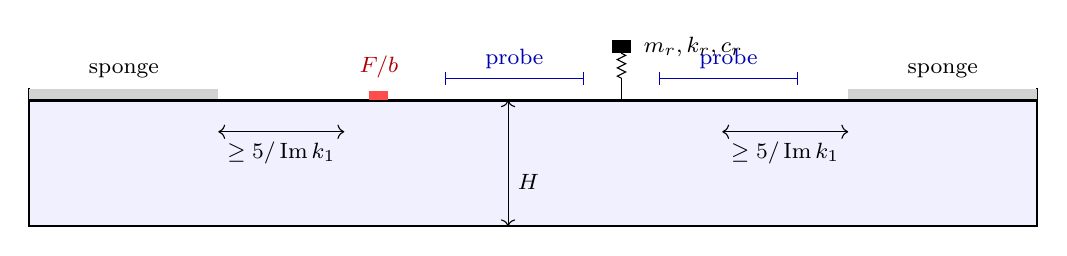
\begin{tikzpicture}[x=0.8cm,y=0.8cm,font=\footnotesize]
        % fluid and walls
        \fill[blue!6] (0,0) rectangle (16,-2);
        \draw[thick] (0,0.2) -- (0,-2) -- (16,-2) -- (16,0.2);
        % sponges
        \fill[gray!35] (0,0) rectangle (3,0.18);
        \fill[gray!35] (13,0) rectangle (16,0.18);
        \node[above] at (1.5,0.2) {sponge};
        \node[above] at (14.5,0.2) {sponge};
        % plate
        \draw[very thick] (0,0) -- (16,0);
        % buffers
        \draw[<->] (3,-0.5) -- (5,-0.5) node[midway,below] {$\ge 5/\operatorname{Im}k_1$};
        \draw[<->] (11,-0.5) -- (13,-0.5) node[midway,below] {$\ge 5/\operatorname{Im}k_1$};
        % source
        \fill[red!70] (5.4,0) rectangle (5.7,0.15);
        \node[above,red!70!black] at (5.55,0.2) {$F/b$};
        % probes
        \draw[|-|, blue!70!black] (6.6,0.35) -- (8.8,0.35) node[midway,above] {probe};
        \draw[|-|, blue!70!black] (10.0,0.35) -- (12.2,0.35) node[midway,above] {probe};
        % resonator
        \draw (9.4,0) -- (9.4,0.35);
        \draw[decorate,decoration={zigzag,amplitude=1.5pt,segment length=3pt}] (9.4,0.35) -- (9.4,0.75);
        \fill (9.25,0.75) rectangle (9.55,0.95);
        \node[right] at (9.6,0.85) {$m_r,k_r,c_r$};
        % depth
        \draw[<->] (7.6,0) -- (7.6,-2);
        \node[right] at (7.6,-1.3) {$H$};
    \end{tikzpicture}
    \caption{Configuration-A channel used for the verification (not to scale): plate over the whole free surface, sponge layers in front of rigid walls, patch source of width $b$, probe windows on which the wave amplitudes are fitted, and (Section~\ref{subsubsec:num_L1_3}) one resonator between the probes. In Sections~\ref{subsubsec:num_L1_1} and~\ref{subsubsec:num_L1_2} the probes are placed on both sides of the source.}
    \label{fig:num_channel_A}
\end{figure}

\paragraph{Forcing.} The waves are generated by a uniform pressure $F/b$ applied over a patch of two plate elements, $b=2h$, which enters the linear form as $(F/b,u)_{\Gamma_m}$. The response of the bare host to this load is known exactly outside the patch,
\begin{equation}\label{eq:num_patch_green}
    G_b(x)=\mathrm{i}\sum_m\operatorname{sinc}\!\Big(\frac{k_mb}{2}\Big)\frac{\mathrm{e}^{\mathrm{i}k_m|x|}}{\mathcal{D}_0'(k_m)},\qquad |x|\ge b/2,
\end{equation}
which reduces to equation~\eqref{eq:lat_green_1d} as $b\to0$. The residue series includes the propagating root, the complex flexural pair and $100$ evanescent roots, enough to evaluate $G(0)$ to a relative accuracy of $10^{-11}$.

\paragraph{Discretisation.} The fluid potential and the plate deflection are approximated with Lagrange polynomials of degree $p\in\{2,3\}$ on a structured mesh, with the C/DG treatment of the plate bending term of Section~\ref{sec:numerical_formulation} (penalty parameter $\gamma=6$). The horizontal element size is $h=\lambda_0/n_\lambda$, with $n_\lambda$ elements per plate wavelength: $n_\lambda\in\{20,40,80\}$ for $p=2$ and $n_\lambda\in\{10,20,40\}$ for $p=3$. Vertically, the mesh is graded geometrically towards the plate, with a top cell of size $h/2$ and a growth ratio bounded by $1+0.2\,(20/n_\lambda)$. Reducing the growth ratio with $h$ makes every cell, down to the bottom, shrink with the mesh size; with a fixed ratio, the cells near the bottom keep their size under refinement, which limited the observed order to $1.25$ at frequencies where the wave reaches the bottom ($k_0H\approx1$--$4$). The largest problems have $1.2\times10^6$ degrees of freedom.

\paragraph{Post-processing.} The plate deflection is sampled on probe windows of three wavelengths and fitted, in the least-squares sense, by
\begin{equation}\label{eq:num_wave_fit}
    \widehat{\eta}_h(x)\simeq A^+\mathrm{e}^{\mathrm{i}k_h(x-x_\mathrm{ref})}+A^-\mathrm{e}^{-\mathrm{i}k_h(x-x_\mathrm{ref})}+\sum_{n=1}^{6}\Big(c_n^+\mathrm{e}^{\mathrm{i}k_n(x-x_a)}+c_n^-\mathrm{e}^{\mathrm{i}k_n(x_b-x)}\Big),
\end{equation}
where $[x_a,x_b]$ is the probe window, $x_\mathrm{ref}$ the source or resonator position, and $k_n$ the flexural pair and the four slowest evanescent roots. The wavenumber $k_h$ is the discrete one, fitted on the field rather than set to $k_0$: with $k_0$ the dispersion error of the discretisation would accumulate in the phase of the amplitudes over the distance to $x_\mathrm{ref}$. Fitting both directions separates the outgoing waves from those returning from the sponges; the source is transparent to the returning waves, so the wave radiated towards one side is the outgoing amplitude on that side minus the incoming amplitude on the other. The accuracy of each quantity $Q_h$ is measured by its relative error against the exact value, $e(Q)=|Q_h/Q-1|$, and the observed order of convergence between the two finest meshes is $\log(e_1/e_2)/\log 2$.

The C/DG plate discretisation converges at order $p-1$ in the energy norm, so that smooth functionals of the solution, such as the wavenumber, the radiated amplitude or the resonance frequency, are expected to converge at order $2(p-1)$. A test is passed when the error on the finest mesh is below $10^{-3}$ for every quantity, and, for $p=2$, when the observed order is at least $2(p-1)-0.3=1.7$. For $p=3$ the errors on the finest meshes reach values between round-off and $10^{-6}$, at which the observed order is no longer a meaningful measure of the discretisation; it is reported but not used as a criterion.

\subsubsection{Bare host: dispersion and Green function}\label{subsubsec:num_L1_1}

\paragraph{Test description.} A patch force $F$ is applied at the centre of the channel without resonators, and three quantities are compared with the theory: (i) the discrete propagating wavenumber $k_h$, fitted on both sides of the source, against the root $k_0$ of equation~\eqref{eq:host_symbol}; (ii) the radiative width obtained from the radiated amplitude $A$, $\gamma_h=A/(\mathrm{i}F\operatorname{sinc}(k_0b/2))$, against $\gamma_r=\operatorname{Im}G(0)=1/\mathcal{D}_0'(k_0)$, equation~\eqref{eq:lat_green_1d}; and (iii) the near field between the patch edge and one wavelength from the source, after subtraction of the waves returning from the sponges, against $FG_b(x)$, equation~\eqref{eq:num_patch_green}, with real and imaginary parts compared separately. The real part of $G$ sets the renormalised resonance of a resonator, equation~\eqref{eq:renorm_single}, and the imaginary part its radiation, equation~\eqref{eq:ImG}. The test is performed first at $\omega=10~\si{\radian\per\second}$ ($T_\rho=0$) on a wide range of meshes, and then for $30$ frequencies logarithmically spaced in $[0.3,15]~\si{\radian\per\second}$ and both pre-tensions. In the frequency sweep only the far-field quantities (i) and (ii) are considered: at low frequency the element size, about $10~\si{\meter}$ at $\omega=0.3~\si{\radian\per\second}$, is much larger than the decay lengths of the near field, which do not scale with the wavelength.

\paragraph{Results.} Table~\ref{tab:num_L1_1} and Figure~\ref{fig:num_L1_1_convergence} show the convergence at $\omega=10~\si{\radian\per\second}$. With $p=2$ all four quantities converge at order $2.0$ from $10$ elements per wavelength on, with the wavenumber about four times more accurate than the radiated amplitude and the near field. With five elements per wavelength the solution is not yet in the asymptotic range: the radiative width is in error by $28\%$. With $p=3$ the errors are three to five orders of magnitude smaller at equal mesh size and fall below $10^{-6}$ with $40$ elements per wavelength, where the real part of the near field and the radiative width level off at about $10^{-6}$ and $2.5\times10^{-7}$, respectively. The frequency sweep (Figures~\ref{fig:num_L1_1_sweep_k} and~\ref{fig:num_L1_1_sweep_gamma}) confirms this picture over the whole range: with $p=2$ the observed order of the wavenumber error is close to $4$ at low frequency, where the bending term is negligible and the wave is essentially a long gravity wave under an inertial plate, and decreases to the order $2$ of the C/DG bending discretisation above $\omega\approx3~\si{\radian\per\second}$, where bending controls the dispersion. The errors increase with frequency and are smaller with pre-tension; on the finest meshes they remain below $1.0\times10^{-4}$ (wavenumber) and $4.1\times10^{-4}$ (radiative width) for $p=2$, and below $2.5\times10^{-8}$ and $7\times10^{-7}$ for $p=3$. At $\omega\le1~\si{\radian\per\second}$ the sponges reflect all the incident energy, and the extraction of the amplitudes, which is exact under reflection, still gives errors between $10^{-10}$ and $10^{-6}$.

\begin{table}[t]
    \centering
    \caption{Bare host at $\omega=10~\si{\radian\per\second}$, $T_\rho=0$: relative errors of the discrete wavenumber, of the radiative width obtained from the far field, and of the real and imaginary parts of the near field, against $k_0$, $\gamma_r=1/\mathcal{D}_0'(k_0)$ and $FG_b(x)$.}
    \label{tab:num_L1_1}
    \footnotesize
    \begin{tabular}{rrrcccc}
        \hline
        $p$ & $n_\lambda$ & DOFs & $k_h$ & $\gamma_h$ & $\operatorname{Re}\widehat{\eta}_h$ & $\operatorname{Im}\widehat{\eta}_h$ \\
        \hline
        2 & 5  & 6\,480   & $6.3\times10^{-3}$ & $2.8\times10^{-1}$ & $8.2\times10^{-2}$ & $1.5\times10^{-1}$ \\
        2 & 10 & 19\,368  & $6.2\times10^{-3}$ & $2.3\times10^{-2}$ & $3.0\times10^{-2}$ & $3.5\times10^{-2}$ \\
        2 & 20 & 67\,662  & $1.5\times10^{-3}$ & $6.4\times10^{-3}$ & $8.0\times10^{-3}$ & $9.2\times10^{-3}$ \\
        2 & 40 & 251\,238 & $3.9\times10^{-4}$ & $1.6\times10^{-3}$ & $2.1\times10^{-3}$ & $2.3\times10^{-3}$ \\
        2 & 80 & 966\,150 & $9.7\times10^{-5}$ & $4.1\times10^{-4}$ & $5.2\times10^{-4}$ & $5.7\times10^{-4}$ \\
        3 & 5  & 13\,961  & $5.2\times10^{-4}$ & $7.4\times10^{-3}$ & $2.8\times10^{-3}$ & $2.5\times10^{-3}$ \\
        3 & 10 & 42\,350  & $9.0\times10^{-6}$ & $8.3\times10^{-5}$ & $1.7\times10^{-4}$ & $6.2\times10^{-5}$ \\
        3 & 20 & 149\,792 & $4.9\times10^{-7}$ & $7.2\times10^{-6}$ & $1.2\times10^{-5}$ & $3.4\times10^{-6}$ \\
        3 & 40 & 560\,396 & $4.3\times10^{-9}$ & $2.5\times10^{-7}$ & $1.1\times10^{-6}$ & $2.9\times10^{-7}$ \\
        \hline
    \end{tabular}
\end{table}

\begin{figure}[t]
    \centering
    \begin{subfigure}{0.49\linewidth}
        \includegraphics[width=\linewidth]{figures/L1_1_convergence_p2.png}
        \caption{$p=2$}
    \end{subfigure}
    \begin{subfigure}{0.49\linewidth}
        \includegraphics[width=\linewidth]{figures/L1_1_convergence_p3.png}
        \caption{$p=3$}
    \end{subfigure}
    \caption{Bare host at $\omega=10~\si{\radian\per\second}$, $T_\rho=0$: relative errors against the number of elements per wavelength. Dashed: order $2(p-1)$.}
    \label{fig:num_L1_1_convergence}
\end{figure}

\begin{figure}[t]
    \centering
    \includegraphics[width=\linewidth]{figures/L1_1_sweep_k.png}
    \caption{Discrete wavenumber over the frequency range, $T_\rho=0$ (left) and $T_\rho=9.8~\si{\meter\cubed\per\second\squared}$ (right). Top: relative error $|k_h/k_0-1|$ for $p=2$ (black) and $p=3$ (blue) on three meshes (dotted, dashed, solid from coarse to fine). Bottom: observed order between the two finest meshes; dashed lines at $2(p-1)$.}
    \label{fig:num_L1_1_sweep_k}
\end{figure}

\begin{figure}[t]
    \centering
    \includegraphics[width=\linewidth]{figures/L1_1_sweep_gamma.png}
    \caption{Radiative width from the far field over the frequency range; layout as in Figure~\ref{fig:num_L1_1_sweep_k}.}
    \label{fig:num_L1_1_sweep_gamma}
\end{figure}

\subsubsection{Radiative width and energy flux}\label{subsubsec:num_L1_2}

\paragraph{Test description.} The radiative width $\gamma_r=\operatorname{Im}G(0)$ controls the critical damping and the absorption of every resonator configuration (Section~\ref{subsubsec:energy_flux_single}), and the energy flux~\eqref{eq:energy_flux} normalises the reflection, transmission and absorption coefficients. Both are verified by computing $\gamma_r$ in three independent ways from the same finite element solution of the bare host forced by the patch:
\begin{enumerate}
    \item \emph{far field}: from the radiated amplitudes, as in Section~\ref{subsubsec:num_L1_1};
    \item \emph{source patch}: in the non-dissipative case $\operatorname{Im}G(x)=\cos(k_0x)/\mathcal{D}_0'(k_0)$ for all $x$, equation~\eqref{eq:lat_green_1d}, so that the average of the patch response over the patch is $\operatorname{Im}\langle G_b\rangle=\operatorname{sinc}^2(k_0b/2)/\mathcal{D}_0'(k_0)$; the finite element average $\langle\widehat{\eta}_h\rangle$, computed by Gauss quadrature on the two patch elements and corrected for the waves returning from the sponges, gives $\gamma_h=\operatorname{Im}\langle\widehat{\eta}_h\rangle/(F\operatorname{sinc}^2(k_0b/2))$;
    \item \emph{work--flux balance}: the work done by the load, $P=\tfrac12\omega\operatorname{Im}(\overline{F}\langle\widehat{\eta}_h\rangle)$, which is equation~\eqref{eq:point_power} for a distributed load, is compared with the net flux $\tfrac14\omega\mathcal{D}_0'(k_0)\sum(|A_\mathrm{out}|^2-|A_\mathrm{in}|^2)$ through both probe windows, equation~\eqref{eq:energy_flux}; the error is $|P/P_\mathrm{flux}-1|$.
\end{enumerate}
The test is performed at $\omega\in\{2,5,10\}~\si{\radian\per\second}$ for both pre-tensions.

\paragraph{Results.} The three measures agree with each other and with $\gamma_r$ for all cases (Table~\ref{tab:num_L1_2} and Figure~\ref{fig:num_L1_2}). With $p=2$ they converge at order $2.0$ (observed orders $1.98$--$2.26$) to errors between $2.5\times10^{-6}$ and $4.1\times10^{-4}$ with $80$ elements per wavelength. The errors increase with frequency, as the bending term becomes dominant, and are two to eight times smaller with pre-tension. With $p=3$ all errors are below $3.3\times10^{-7}$ with $40$ elements per wavelength; at $\omega=10~\si{\radian\per\second}$ they reach the same level of $2$--$3\times10^{-7}$ found for the far field in Section~\ref{subsubsec:num_L1_1}. That the work done by the load equals the flux of the radiated waves to this accuracy confirms that equation~\eqref{eq:energy_flux}, derived from the Green function, is the energy flux of the discrete coupled fluid--structure system, and therefore that the reflection, transmission and absorption coefficients of Section~\ref{subsubsec:num_L1_3} are correctly normalised.

\begin{table}[t]
    \centering
    \caption{Radiative width: exact value $\gamma_r=1/\mathcal{D}_0'(k_0)$ (density-normalised symbol) and relative errors of the three finite element measures on the finest mesh ($n_\lambda=80$ for $p=2$, $40$ for $p=3$). $T_\rho$ in \si{\meter\cubed\per\second\squared}, $\omega$ in \si{\radian\per\second}.}
    \label{tab:num_L1_2}
    \footnotesize
    \begin{tabular}{rrcrccc}
        \hline
        $T_\rho$ & $\omega$ & $\gamma_r$ & $p$ & far field & source patch & work--flux \\
        \hline
        0   & 2  & 0.0415 & 2 & $5.9\times10^{-6}$ & $5.9\times10^{-6}$ & $5.9\times10^{-6}$ \\
            &    &        & 3 & $4.8\times10^{-9}$ & $4.8\times10^{-9}$ & $1.4\times10^{-9}$ \\
        0   & 5  & 0.0534 & 2 & $3.8\times10^{-4}$ & $3.8\times10^{-4}$ & $3.8\times10^{-4}$ \\
            &    &        & 3 & $1.6\times10^{-7}$ & $4.9\times10^{-8}$ & $5.7\times10^{-8}$ \\
        0   & 10 & 0.0186 & 2 & $4.1\times10^{-4}$ & $4.1\times10^{-4}$ & $4.1\times10^{-4}$ \\
            &    &        & 3 & $2.5\times10^{-7}$ & $2.1\times10^{-7}$ & $2.6\times10^{-7}$ \\
        9.8 & 2  & 0.0263 & 2 & $2.5\times10^{-6}$ & $2.5\times10^{-6}$ & $2.6\times10^{-6}$ \\
            &    &        & 3 & $1.4\times10^{-8}$ & $1.3\times10^{-8}$ & $2.4\times10^{-9}$ \\
        9.8 & 5  & 0.0224 & 2 & $4.9\times10^{-5}$ & $4.8\times10^{-5}$ & $4.9\times10^{-5}$ \\
            &    &        & 3 & $1.4\times10^{-7}$ & $9.9\times10^{-8}$ & $2.1\times10^{-9}$ \\
        9.8 & 10 & 0.0127 & 2 & $1.3\times10^{-4}$ & $1.3\times10^{-4}$ & $1.3\times10^{-4}$ \\
            &    &        & 3 & $3.1\times10^{-7}$ & $3.2\times10^{-7}$ & $2.8\times10^{-7}$ \\
        \hline
    \end{tabular}
\end{table}

\begin{figure}[t]
    \centering
    \includegraphics[width=\linewidth]{figures/L1_2_convergence_p2.png}\\
    \includegraphics[width=\linewidth]{figures/L1_2_convergence_p3.png}
    \caption{Radiative width from the far field, from the source patch and from the work--flux balance, for $p=2$ (top) and $p=3$ (bottom); colour: frequency, marker: pre-tension. Dashed: order $2(p-1)$.}
    \label{fig:num_L1_2}
\end{figure}

\subsubsection{Single resonator}\label{subsubsec:num_L1_3}

\paragraph{Test description.} One resonator ($m_{\rho,r}=0.01~\si{\meter\squared}$, $\omega_r=10~\si{\radian\per\second}$) is attached to the plate four and a half wavelengths downstream of the source, between two probe windows of three wavelengths placed one wavelength from it on either side (Figure~\ref{fig:num_channel_A}). The mesh is sized with the wavelength at $\omega_r$, so that all frequencies of a case are computed on the same mesh. The resonator is placed either on a mesh node or at the midpoint of an element, which tests the point evaluations $\widehat{\eta}(\mathbf{x}_i)$, $u(\mathbf{x}_i)$ of the resonator terms in equation~\eqref{eq:Bilinear_freq}. The dashpot is $c_r=0$ (lossless) or $c_r=c_\mathrm{crit}$, the value that gives critical coupling, $\gamma_d=\gamma_r$, equation~\eqref{eq:critical_coupling}, at the renormalised resonance of the undamped resonator; this corresponds to $\zeta=0.0093$ ($T_\rho=0$) and $0.0064$ ($T_\rho=9.8~\si{\meter\cubed\per\second\squared}$), equation~\eqref{eq:zeta_opt}.

Equation~\eqref{eq:single_force} states that the resonator force is $F_1=\widehat{\eta}_f(x_1)/(1/\alpha-G(0))$, where $\widehat{\eta}_f(x_1)$ is the field of the bare structure at the attachment point. In the computational setting $\widehat{\eta}_f$ contains, besides the incident wave of amplitude $A^+$ and the wave $B^-$ returning from the downstream sponge, the tail of the near field of the source, $E=FG_{b,\mathrm{near}}(x_1-x_s)$, where $G_{b,\mathrm{near}}$ denotes equation~\eqref{eq:num_patch_green} without the propagating term. Although small, about $2\times10^{-3}$ of the incident wave for the slowest evanescent mode at a distance of $10~\si{\meter}$, this contribution must be included: treating the incident wave as the only drive introduces a phase error of the same size in $\mathcal{R}$, which shifts the computed resonance by an amount proportional to the resonance width ($-1.8\times10^{-5}$ in relative terms for $T_\rho=0$) and independent of the mesh. The coefficients are therefore obtained as follows. The exact near fields of the source and of the resonator, $FG_{b,\mathrm{near}}(x-x_s)$ and $F_1G_\mathrm{near}(x-x_1)$ with $F_1=\omega^2m_{\rho,r}q_1$ from the computed resonator motion, are subtracted from the probe samples, which are then fitted by the two propagating waves of equation~\eqref{eq:num_wave_fit} only, with the discrete wavenumber measured on the bare plate. The resonator radiates the same amplitude $S$ to both sides, $S=B^+-A^+=A^--B^-$, so that
\begin{equation}\label{eq:num_point_scattering}
    \mathcal{R}=\frac{S}{A^++B^-+E},\qquad \mathcal{T}=1+\mathcal{R},\qquad \mathcal{A}=1-|\mathcal{R}|^2-|\mathcal{T}|^2,
\end{equation}
in agreement with equations~\eqref{eq:lat_RT} and~\eqref{eq:lat_energy_1d} for one resonator. The two estimates of $S$ agree to better than $10^{-6}$ relative, which provides an independent consistency check.

Since $\mathcal{R}=\mathrm{i}\gamma_r/(x-\mathrm{i}\Gamma)$, with $\Gamma=\gamma_r+\gamma_d$, holds for the discrete system with its own discrete Green function, $1/\mathcal{R}=-(\Gamma+\mathrm{i}x)/\gamma_r$ is a smooth function of frequency. The renormalised resonance $\widetilde{\omega}_r$, where the detuning vanishes, equation~\eqref{eq:renorm_single}, is the root of $\operatorname{Im}(1/\mathcal{R})$, and the half-power frequencies, where $x=\pm\Gamma$, are the roots of $\operatorname{Im}(1/\mathcal{R})\mp\operatorname{Re}(1/\mathcal{R})$. These roots are computed by secant iteration on finite element solutions (13 to 16 solutions per case) and compared with the same roots of the exact single-resonator solution, equation~\eqref{eq:single_force}, with the same resonator. In addition, $\mathcal{R}(\widetilde{\omega}_r)=-1$ and $\mathcal{T}(\widetilde{\omega}_r)=0$ are checked for the lossless resonator, and $\mathcal{A}(\widetilde{\omega}_r)=\tfrac12$ at critical coupling, equation~\eqref{eq:lat_absorbed_1d}. Finally, the response curves are computed at $41$ frequencies in $\omega_r(1\pm5/Q_\mathrm{rad})$, with $Q_\mathrm{rad}=\mathcal{D}_0'(k_0)/(\omega_r^2m_{\rho,r})=53.7$ ($T_\rho=0$) and $78.7$ ($T_\rho=9.8~\si{\meter\cubed\per\second\squared}$), for $c_r/c_\mathrm{crit}\in\{0,\tfrac12,1,2\}$, with $p=3$ and ten elements per wavelength.

\paragraph{Results.} The renormalised resonance of the lossless resonator is $\widetilde{\omega}_r=10.0234~\si{\radian\per\second}$ for $T_\rho=0$ and $9.9889~\si{\radian\per\second}$ for $T_\rho=9.8~\si{\meter\cubed\per\second\squared}$, i.e.\ shifted from $\omega_r$ by $+0.23\%$ and $-0.11\%$ by the point compliance $\operatorname{Re}G(0)$ of the floating plate, whose sign changes with the pre-tension. Table~\ref{tab:num_L1_3} and Figure~\ref{fig:num_L1_3_convergence} show that the finite element reproduces this shift and the resonance bandwidth to high accuracy. With $p=2$ the relative errors of $\widetilde{\omega}_r$ and of the bandwidth converge at order $1.8$--$2.1$, to $5$--$7\times10^{-6}$ and $4\times10^{-5}$--$4\times10^{-4}$, respectively, with $80$ elements per wavelength, for both attachments and both dashpots. With $p=3$ and the resonator on a node, $\widetilde{\omega}_r$ is reproduced to $3\times10^{-11}$--$3\times10^{-9}$ and the bandwidth to $10^{-9}$--$4\times10^{-8}$. With the resonator at the midpoint of an element, the $p=3$ errors are larger, $0.7$--$1.8\times10^{-6}$ for $\widetilde{\omega}_r$, and converge at order $\approx3$: a point load inside an element reduces the regularity of the discrete solution within that element. At resonance, $|\mathcal{R}+1|$ is below $10^{-7}$ for the lossless resonator, and at critical coupling the absorbed fraction is $\tfrac12$ to within $10^{-7}$ ($2\times10^{-8}$ with $p=3$); the $p=3$ value is the difference between $\tfrac12$ and the exact $\mathcal{A}(\widetilde{\omega}_r)$, since $c_\mathrm{crit}$ is defined at the resonance of the undamped resonator. The resonator motion satisfies $q_1/\widehat{\eta}_1=k_{\rho,r}^\omega/(k_{\rho,r}^\omega-\omega^2m_{\rho,r})$, equation~\eqref{eq:resonator_motion}, to round-off.

The response curves of Figure~\ref{fig:num_L1_3_curves} lie on the exact ones for all dashpots. Total reflection occurs at $\widetilde{\omega}_r$ for the lossless resonator; the absorbed fraction reaches its bound of one half only at critical coupling, and the absorption peak broadens and decreases for $c_r=2c_\mathrm{crit}$, as predicted by equation~\eqref{eq:lat_absorbed_1d}. The computed half-power bandwidths, $\Delta\omega/\widetilde{\omega}_r=0.0186$ and $0.0373$ for $T_\rho=0$ and $0.0127$ and $0.0255$ for $T_\rho=9.8~\si{\meter\cubed\per\second\squared}$ (lossless and critically damped), agree within $0.3\%$ with the estimate $(1+c_r/c_\mathrm{crit})/Q_\mathrm{rad}$, i.e.\ $2/Q_\mathrm{rad}$ at critical coupling.

\begin{table}[t]
    \centering
    \caption{Single resonator: relative errors on the finest mesh ($n_\lambda=80$ for $p=2$, $40$ for $p=3$) of the renormalised resonance $\widetilde{\omega}_r$ and of the half-power bandwidth $\Delta\omega$, and the peak response error, $|\mathcal{R}(\widetilde{\omega}_r)+1|$ for $c_r=0$ and $|\mathcal{A}(\widetilde{\omega}_r)-\tfrac12|$ for $c_r=c_\mathrm{crit}$. Observed orders for $p=2$ in brackets; $T_\rho$ in \si{\meter\cubed\per\second\squared}.}
    \label{tab:num_L1_3}
    \footnotesize
    \begin{tabular}{rrlrccc}
        \hline
        $T_\rho$ & $c_r/c_\mathrm{crit}$ & attachment & $p$ & $\widetilde{\omega}_r$ & $\Delta\omega$ & peak \\
        \hline
        0   & 0 & node        & 2 & $5.5\times10^{-6}$ (1.93) & $3.7\times10^{-4}$ (2.00) & $2.0\times10^{-8}$ \\
            &   &             & 3 & $1.0\times10^{-10}$ & $4.6\times10^{-9}$ & $9.3\times10^{-11}$ \\
        0   & 1 & node        & 2 & $5.5\times10^{-6}$ (1.93) & $1.9\times10^{-4}$ (2.00) & $8.7\times10^{-8}$ \\
            &   &             & 3 & $3.1\times10^{-11}$ & $1.2\times10^{-9}$ & $2.1\times10^{-8}$ \\
        0   & 0 & mid-element & 2 & $5.4\times10^{-6}$ (1.89) & $3.7\times10^{-4}$ (2.00) & $4.3\times10^{-8}$ \\
            &   &             & 3 & $6.5\times10^{-7}$ & $4.1\times10^{-7}$ & $1.8\times10^{-10}$ \\
        9.8 & 0 & node        & 2 & $7.2\times10^{-6}$ (1.87) & $1.0\times10^{-4}$ (2.02) & $2.5\times10^{-9}$ \\
            &   &             & 3 & $2.9\times10^{-9}$ & $3.9\times10^{-8}$ & $1.8\times10^{-11}$ \\
        9.8 & 1 & node        & 2 & $7.2\times10^{-6}$ (1.87) & $4.3\times10^{-5}$ (2.07) & $1.1\times10^{-8}$ \\
            &   &             & 3 & $2.7\times10^{-10}$ & $1.1\times10^{-9}$ & $3.0\times10^{-9}$ \\
        9.8 & 0 & mid-element & 2 & $6.8\times10^{-6}$ (1.80) & $1.0\times10^{-4}$ (2.02) & $4.7\times10^{-10}$ \\
            &   &             & 3 & $1.8\times10^{-6}$ & $3.1\times10^{-6}$ & $1.4\times10^{-11}$ \\
        \hline
    \end{tabular}
\end{table}

\begin{figure}[t]
    \centering
    \includegraphics[width=\linewidth]{figures/L1_3_convergence_p2.png}\\
    \includegraphics[width=\linewidth]{figures/L1_3_convergence_p3.png}
    \caption{Single resonator: relative errors of the renormalised resonance, of the half-power bandwidth and of the peak response against the number of elements per wavelength, for $p=2$ (top) and $p=3$ (bottom); colour: dashpot and attachment, marker: pre-tension. Dashed: order $2(p-1)$.}
    \label{fig:num_L1_3_convergence}
\end{figure}

\begin{figure}[t]
    \centering
    \includegraphics[width=\linewidth]{figures/L1_3_response_curves.png}
    \caption{Single resonator: reflection coefficient $|\mathcal{R}|$ (top) and absorbed fraction $\mathcal{A}$ (bottom) for $T_\rho=0$ (left) and $T_\rho=9.8~\si{\meter\cubed\per\second\squared}$ (right) and $c_r/c_\mathrm{crit}\in\{0,\tfrac12,1,2\}$. Lines: exact solution, equation~\eqref{eq:single_force}; markers: finite element ($p=3$, ten elements per wavelength). Dashed: bound $\mathcal{A}=\tfrac12$, equation~\eqref{eq:lat_absorbed_1d}.}
    \label{fig:num_L1_3_curves}
\end{figure}

\subsubsection{Single resonator across frequency: optimal damping}\label{subsubsec:num_L1_3b}

\paragraph{Test description.} Section~\ref{subsubsec:energy_flux_single} predicts that critical coupling, $\gamma_d=\gamma_r$, gives the absorbed fraction $\mathcal{A}=\tfrac12$ at resonance, and that the corresponding damping ratio, equation~\eqref{eq:zeta_opt}, collapses at low frequency, where the fluid makes up most of $\mathcal{D}_0'(k_0)$: $\zeta_{\rm opt}=9.3\times10^{-3}$ at $\omega_r=10~\si{\radian\per\second}$ but $4.3\times10^{-5}$ at $\omega_r=1~\si{\radian\per\second}$ ($T_\rho=0$, Figure~\ref{fig:lattice_design}(b)). The test of Section~\ref{subsubsec:num_L1_3} is repeated for $\omega_r\in\{1,2,5,10\}~\si{\radian\per\second}$ (same resonator mass, $m_{\rho,r}=0.01~\si{\meter\squared}$), both pre-tensions and $c_r/c_\mathrm{crit}\in\{\tfrac14,\tfrac12,1,2,4\}$, with $p=3$ and $10$ and $20$ elements per wavelength $\lambda_0(\omega_r)$; at $\omega_r=1~\si{\radian\per\second}$, $\lambda_0=51.6~\si{\meter}$ and the radiative quality factor is $Q_\mathrm{rad}=1.15\times10^4$. For each dashpot the renormalised resonance $\widetilde{\omega}_r$ of the finite element model is located as in Section~\ref{subsubsec:num_L1_3}, and $\mathcal{A}(\widetilde{\omega}_r)$ is compared with the exact value $4x/(1+x)^2$, $x=\gamma_d/\gamma_r$. The dashpot that maximises the finite element absorption is located by a parabola in $\log c_r$ through $c_r/c_\mathrm{crit}\in\{\tfrac12,1,2\}$, and the corresponding damping ratio is compared with $\zeta_{\rm opt}$. At $\omega_r=1~\si{\radian\per\second}$ the sponges of Section~\ref{subsubsec:num_setup_A} are replaced by viscous dashpot layers on the plate, $c_{\rho}\sigma(x)\dot{\eta}$ with $\sigma$ rising quadratically from $0$ to $1$, since the bending sponges are transparent at this frequency.

\paragraph{Results.} At every frequency the finite element model reaches the bound of one half at critical coupling, $|\mathcal{A}(\widetilde{\omega}_r)-\tfrac12|\le3\times10^{-8}$, and reproduces $\mathcal{A}(\widetilde{\omega}_r)$ for the other dashpots to $4\times10^{-8}$ for $\omega_r\ge2~\si{\radian\per\second}$ and $7.5\times10^{-6}$ at $\omega_r=1~\si{\radian\per\second}$. The maximum of the finite element absorption lies at $c_\mathrm{crit}$ to within $4.5\times10^{-4}$ (relative), and the damping ratio at the maximum follows equation~\eqref{eq:zeta_opt} over more than two decades (Figure~\ref{fig:num_L1_3b}): from $9.26\times10^{-3}$ at $\omega_r=10~\si{\radian\per\second}$ to $4.35\times10^{-5}$ at $\omega_r=1~\si{\radian\per\second}$ for $T_\rho=0$, and from $6.37\times10^{-3}$ to $4.14\times10^{-5}$ for $T_\rho=9.8~\si{\meter\cubed\per\second\squared}$. The remaining differences, at most $0.6\%$ at $\omega_r=10~\si{\radian\per\second}$, are those between $c_\mathrm{crit}$, defined at the renormalised resonance, and the explicit formula~\eqref{eq:zeta_opt}, evaluated at $\omega_r$. The renormalised resonance itself is reproduced to $6\times10^{-11}$--$3\times10^{-8}$ for $\omega_r\ge5~\si{\radian\per\second}$ and to $5\times10^{-7}$--$2\times10^{-6}$ at $\omega_r=2~\si{\radian\per\second}$. At $\omega_r=1~\si{\radian\per\second}$ the error is $3.8\times10^{-5}$ ($T_\rho=0$) and $1.4\times10^{-5}$ ($T_\rho=9.8~\si{\meter\cubed\per\second\squared}$) with $20$ elements per wavelength, i.e.\ $0.22$ and $0.09$ times the half-power width, and still decreasing with the mesh: the elements, sized with the wavelength ($2.6~\si{\meter}$), do not resolve the flexural near field (decay length $0.5~\si{\meter}$ for $T_\rho=0$), which sets $\operatorname{Re}G(0)$ and hence the shift of the resonance, $\widetilde{\omega}_r/\omega_r-1=-4.2\times10^{-4}$, about five times the bandwidth $\widetilde{\omega}_r/Q_\mathrm{rad}$ of the lossless resonator. The absorbed fraction at the finite element resonance is not affected, since $\mathcal{R}=\mathrm{i}\gamma_r/(x-\mathrm{i}\Gamma)$ holds for the discrete system with its own Green function.

\begin{figure}[t]
    \centering
    \includegraphics[width=\linewidth]{figures/L1_3b_zeta_opt.png}
    \caption{Damping ratio of the dashpot that maximises the absorbed fraction of a single resonator ($m_{\rho,r}=0.01~\si{\meter\squared}$) against the resonator frequency. Markers: finite element ($p=3$, $20$ elements per wavelength); lines: equation~\eqref{eq:zeta_opt}; dotted: bound~\eqref{eq:zeta_bound}.}
    \label{fig:num_L1_3b}
\end{figure}

\subsubsection{Discussion}\label{subsubsec:num_discussion_A}

The three tests show that the monolithic finite element formulation reproduces the Green-function theory of Section~\ref{sec:discrete_lattice} for an infinite floating structure, to an accuracy limited only by the discretisation. The propagating wavenumber, the radiated amplitude and the near field of the bare host converge at order $2(p-1)$, the order expected for smooth quantities with the C/DG treatment of the bending term, over a frequency range of almost two decades in which the host changes from a long gravity wave under an inertial plate to a bending-dominated flexural wave. With $p=2$, twenty elements per wavelength give errors below $1\%$ and forty below $0.25\%$; $p=3$ gives better accuracy with a quarter of the elements per wavelength ($10^{-4}$ with ten) and errors between $10^{-5}$ and $10^{-7}$ with twenty. The quadratic order of the bending discretisation is therefore the limiting factor for $p=2$, and $p=3$ is preferable whenever accurate near fields or resonance frequencies are required.

The radiative width $\gamma_r$ obtained from the far field, from the force patch and from the balance between the work of the load and the energy flux of the radiated waves agree with $1/\mathcal{D}_0'(k_0)$ and with each other. This verifies, for the discrete coupled system, the two results on which the absorption analysis of Section~\ref{subsubsec:energy_flux_single} rests: that only the propagating root contributes to $\operatorname{Im}G(0)$, and that the energy flux of a flexural--gravity wave is $\tfrac14\omega\mathcal{D}_0'(k_0)|A|^2$, with the fluid kinetic energy contained in $\mathcal{D}_0'$.

For a single resonator, the finite element reproduces the renormalisation of the resonance by the point compliance of the floating structure, $\operatorname{Re}G(0)$, the radiative and dissipative widths, total reflection at resonance and the absorption bound of one half at critical coupling. The accuracy of the resonance frequency, $10^{-5}$ with $p=2$ and $10^{-9}$ or better with $p=3$, is several orders of magnitude finer than the relative bandwidth $2/Q_\mathrm{rad}\approx0.03$, so that the resonance of a resonator coupled to the floating structure is resolved by the formulation without loss of accuracy at standard mesh resolutions. Attaching the resonator inside an element rather than at a node is admissible but reduces the convergence order with $p=3$; resonators are therefore best placed on mesh nodes.

Two aspects of the computational setting deserve attention in applications of the formulation to unbounded structures. First, the evanescent fluid modes are not absorbed by sponge layers acting on the structure, and decay only over $1/\operatorname{Im}k_1\approx2H/\pi$; sources and scatterers must be kept at several decay lengths from the sponges and from each other, or their near fields must be accounted for explicitly, as in equation~\eqref{eq:num_point_scattering}. Second, sponge layers acting on bending do not absorb long waves; at low frequency the truncated domain behaves as a closed basin, and its length must be chosen away from the basin resonances. With these precautions the extraction of reflection, transmission and absorption from the finite element field is exact under any amount of reflection from the domain ends, and the verification extends from $\omega=0.3$ to $15~\si{\radian\per\second}$.

\subsection{Floating line lattices: finite arrays and band structure}\label{subsec:num_lattices}

The results of Section~\ref{sec:discrete_lattice} that distinguish a floating lattice from a lattice of resonators in vacuo are obtained from the Green function of the bare host: the complete stop band set by the discrete geometry (Section~\ref{subsubsec:lat_long_wave}), its $a^4$ dependence on the spacing at fixed loading, equation~\eqref{eq:gap_a4}, and the dilution of the hybridisation by the fluid added mass, equation~\eqref{eq:anticrossing}. The monolithic finite element model contains neither the Green function nor the lattice sums: the fluid is discretised in the whole depth, the plate by the C/DG formulation and the resonators by point attachments, so that every Fourier component of the attachment pattern and every evanescent fluid mode is represented to the accuracy of the mesh. In this section the finite element model is compared with the multiple-scattering solution of finite arrays and with the lattice sums of infinite arrays, for line arrays in the vertical section, configuration~A, with the parameters of Table~\ref{tab:dispersion_test_parameters}.

\subsubsection{Numerical setup for periodic lattices}\label{subsubsec:num_setup_lattice}

Band frequencies are computed without Bloch-periodic boundary conditions and without an eigenvalue solver. The computational domain is a periodic channel of depth $H$ and length $Ma$, i.e.\ a supercell of $M$ cells, whose free surface is entirely covered by the plate and which carries $M$ resonators at $x_n=(n-\tfrac12)a$; the domain is closed, so that no sponge layers are needed. A supercell admits the Bloch wavenumbers $q=2\pi j/(Ma)$, $j=0,\ldots,M-1$, and a load selects one of them: each resonator position carries a patch load of amplitude $F\mathrm{e}^{\mathrm{i}qx_n}$, which excites only the Bloch modes with wavenumber $q$. The band frequencies at $q$ are the poles of the projected response
\begin{equation}\label{eq:num_bloch_response}
    g(\omega)=\frac{1}{MF}\sum_{n=1}^{M}\mathrm{e}^{-\mathrm{i}qx_n}\,q_n(\omega),
\end{equation}
with $q_n$ the resonator amplitudes of the finite element solution, and are found as the roots of $\operatorname{Re}(1/g)$, a smooth function of $\omega$ near each pole, by secant iteration started at the lattice-sum value. The zone centre $\Gamma$ is $M=1$, $j=0$, the zone boundary $X$ is $M=2$, $j=1$, and interior wavenumbers follow from larger supercells. In the lossless problem $\operatorname{Im}(1/g)$ vanishes at the poles; its value, below $2\times10^{-11}$ relative in all cases, checks that the load excites a single Bloch wavenumber. The bare host is checked in the same way: without resonators, the pole at $q=\pi/a$ is the frequency $\omega_0(\pi/a)$ of the bare branch. The mesh is uniform in $x$ with $n_c$ elements per cell, so that every resonator lies on a node, and graded vertically as in Section~\ref{subsubsec:num_setup_A}.

\subsubsection{Finite arrays}\label{subsubsec:num_L1_4}

\paragraph{Test description.} Arrays of $N\in\{1,2,5,10,20,40\}$ identical resonators with spacing $a=1~\si{\meter}$, $\omega_r=10~\si{\radian\per\second}$ and damping ratios $\zeta\in\{0,0.01,0.05\}$ are placed in the channel of Section~\ref{subsubsec:num_setup_A}, with a mesh of $n_c$ elements per spacing so that every resonator lies on a node and the mesh is symmetric about the centre of the array, $x_c$. Probe samples on either side of the array, minus the exact near fields of the source and of every resonator (forces $\omega^2m_{\rho,r}q_n$ from the finite element solution), are fitted by the incoming and outgoing propagating waves, with amplitudes $a_L$, $a_R$ and $b_L$, $b_R$ referred to $x_c$. The array is symmetric, so that
\begin{equation}\label{eq:num_two_port}
    b_L=\mathcal{R}a_L+\mathcal{T}a_R,\qquad b_R=\mathcal{T}a_L+\mathcal{R}a_R ,
\end{equation}
which gives $\mathcal{R}$ and $\mathcal{T}$ for any amount of reflection from the ends of the channel; the waves radiated by the array under the drive of the source near field, of relative size $10^{-3}$, are removed from $b_L$, $b_R$ beforehand, as in Section~\ref{subsubsec:num_L1_3}. $\mathcal{R}$, $\mathcal{T}$ and $\mathcal{A}=1-|\mathcal{R}|^2-|\mathcal{T}|^2$ are compared with the solution of the Foldy system~\eqref{eq:lat_foldy} with the residue Green function~\eqref{eq:lat_green_1d}, equations~\eqref{eq:lat_RT} and~\eqref{eq:lat_energy_1d}, at $41$ frequencies in $[8,12]~\si{\radian\per\second}$ and $61$ in $[9.55,10.05]~\si{\radian\per\second}$, with $p=3$ and $n_c=4$ (nine elements per wavelength at $\omega_r$). The mesh convergence is checked for $N=10$ at five frequencies with $n_c\in\{4,8,16\}$.

\paragraph{Results.} The finite element transmission and reflection coincide with the Foldy solution for all arrays, dashpots and pre-tensions (Figure~\ref{fig:num_L1_4_transmission}): the largest difference over all frequencies is $|\mathcal{T}_h-\mathcal{T}|=7.3\times10^{-4}$ and $|\mathcal{R}_h-\mathcal{R}|=8.2\times10^{-4}$, for the longest lossless array ($N=40$, $T_\rho=0$), and at most $2.2\times10^{-4}$ in the damped cases; the absorbed fractions agree to $1.2\times10^{-5}$. Since the Foldy absorbed fraction is the dashpot power, which satisfies the energy identity~\eqref{eq:lat_energy_1d} exactly, this agreement also verifies the energy balance of the finite element $\mathcal{R}$ and $\mathcal{T}$. Under mesh refinement the difference decreases to $4.5\times10^{-7}$--$8.9\times10^{-7}$ with $n_c=16$, and the balance between the net incoming wave flux and the power dissipated in the dashpots closes to between $3\times10^{-10}$ and $4\times10^{-9}$ of the incoming flux, once the response to the near field of the source, which receives its energy by evanescent tunnelling through the probe windows, is removed. In the stop band $[\omega_X,\omega_\Gamma]$ of the lattice (Section~\ref{subsubsec:num_L1_5}) the transmission decreases exponentially with $N$, to $|\mathcal{T}_{40}|=2.7\times10^{-6}$ for $T_\rho=0$.

The rate of this decrease is not set by a single Bloch wavenumber (Figure~\ref{fig:num_L1_4_decay}). Near the lower edge $\omega_X$, the rate $\ln(|\mathcal{T}_{10}|/|\mathcal{T}_{20}|)/(10a)$ equals the imaginary part of the Bloch wavenumber with $\operatorname{Re}q=\pi/a$ from the lattice sums, e.g.\ $0.183$ and $0.350~\si{\per\meter}$ at $\omega=9.7$ and $9.8~\si{\radian\per\second}$ ($T_\rho=0$), against $0.183$ and $0.353~\si{\per\meter}$. Higher in the stop band, where $\operatorname{Im}q$ grows towards $\omega_\Gamma$, the rate falls behind it: for $T_\rho=0$ it peaks at $0.44~\si{\per\meter}$ near $\omega=9.87~\si{\radian\per\second}$ and then decreases towards $\omega_\Gamma$, and for $T_\rho=9.8~\si{\meter\cubed\per\second\squared}$ it stays between $0.11$ and $0.17~\si{\per\meter}$ while $\operatorname{Im}q$ of the zone-boundary mode rises from $0.36$ to $1.7~\si{\per\meter}$. The level it approaches is the attenuation of a second Bloch mode, which continues the slowest evanescent fluid root $k_1=\mathrm{i}\kappa_1$ of equation~\eqref{eq:green_function} into the lattice ($0.10$--$0.15~\si{\per\meter}$, against $\kappa_1=0.158~\si{\per\meter}$ at $H=10~\si{\meter}$). This mode is excited at the first resonator and converted back into the propagating wave at the last one, and it dominates the transmission of long arrays wherever the propagating attenuation exceeds its own. The finite element and Foldy rates agree to $10^{-4}~\si{\per\meter}$ throughout, so that this is a property of the discrete hydroelastic lattice and not of either model. Equation~\eqref{eq:lat_decay}, which neglects the evanescent interactions between resonators, is therefore limited to spacings large compared with $H/\pi$, as stated with it, and the attenuation that a long floating array can provide per unit length is bounded by approximately $\kappa_1\simeq\pi/(2H)$ (for $\omega^2H/g\gg1$), whatever the resonators.

\begin{figure*}[t]
    \centering
    \includegraphics[width=0.85\linewidth]{figures/L1_4_transmission.png}
    \caption{Transmission $|\mathcal{T}_N|$ of arrays of $N$ identical resonators ($a=1~\si{\meter}$, $\omega_r=10~\si{\radian\per\second}$) for $T_\rho=0$ (left), $T_\rho=9.8~\si{\meter\cubed\per\second\squared}$ (right), $\zeta=0$ (top) and $\zeta=0.05$ (bottom). Lines: Foldy solution, equation~\eqref{eq:lat_foldy}; markers: finite element ($p=3$, every third frequency shown).}
    \label{fig:num_L1_4_transmission}
\end{figure*}

\begin{figure}[t]
    \centering
    \includegraphics[width=\linewidth]{figures/L1_4_decay.png}
    \caption{Decay rate of the transmission with the number of lossless resonators inside the stop band $[\omega_X,\omega_\Gamma]$. Line: Foldy solution; markers: finite element; dashed: imaginary part of the Bloch wavenumber with $\operatorname{Re}q=\pi/a$ (lattice sums); dotted: decay rate $\kappa_1$ of the slowest evanescent fluid mode.}
    \label{fig:num_L1_4_decay}
\end{figure}

\subsubsection{Complete stop band}\label{subsubsec:num_L1_5}

\paragraph{Test description.} The band edges $\omega_\Gamma$ (one cell) and $\omega_X$ (two cells with alternating load), the band frequencies at $qa\in\{\pi/4,\pi/2,3\pi/4\}$ (eight cells) and the bare-host frequency $\omega_0(\pi/a)$ are computed for $a=1~\si{\meter}$, $m_{\rho,r}=0.01~\si{\meter\squared}$, $\omega_r=10~\si{\radian\per\second}$, both pre-tensions, with $p=2$ and $n_c\in\{8,16,32,64\}$, and $p=3$ and $n_c\in\{4,8,16,32\}$ ($\lambda_0/a=2.29$ and $3.26$). The references are the roots of equation~\eqref{eq:bloch_condition}. The test also checks that the finite element edges are \emph{not} those obtained by truncating the local branches~\eqref{eq:omega_k_x_closed_form} at $qa=\pi$, $[\omega_-(\pi/a),\omega_r]$, and that the gap is not the anticrossing width~\eqref{eq:anticrossing}.

\paragraph{Results.} The finite element model has the complete stop band of the lattice sums (Table~\ref{tab:num_L1_5} and Figure~\ref{fig:num_L1_5}). With $p=3$ and $32$ elements per cell, both edges agree with the lattice sums to $10^{-10}$ or better, the width of the gap to $5\times10^{-9}$, the interior band frequencies to $10^{-10}$ and the bare host to $3\times10^{-10}$; with $p=2$ all quantities converge at order $1.94$--$2.00$. The upper edge agrees with the estimate $\omega_r/\sqrt{1+\Pi_L}$ of equation~\eqref{eq:lat_gamma} to $8\times10^{-8}$. The truncated local edges, $[9.8125,10]~\si{\radian\per\second}$ for $T_\rho=0$ and $[9.9592,10]~\si{\radian\per\second}$ for $T_\rho=9.8~\si{\meter\cubed\per\second\squared}$, differ from the finite element edges by more than $10^8$ times the finite element error, and the gaps, $0.0340\,\omega_r$ and $0.00738\,\omega_r$, are $4.8$ and $18.6$ times smaller than the anticrossing widths $0.163$ and $0.137$. The finite element model, which retains every Fourier component of the attachment pattern, therefore confirms that both edges of the stop band are set by the discrete geometry: the upper edge by the near-field renormalisation of the resonance at the zone centre, the lower edge by the zone-folded component at the zone boundary.

\begin{table}[t]
    \centering
    \caption{Band edges of a line array ($a=1~\si{\meter}$, $m_{\rho,r}=0.01~\si{\meter\squared}$, $\omega_r=10~\si{\radian\per\second}$): lattice sums, equation~\eqref{eq:bloch_condition}, and relative errors of the finite element model on the finest mesh ($n_c=64$ for $p=2$, $32$ for $p=3$). $T_\rho$ in \si{\meter\cubed\per\second\squared}, frequencies in \si{\radian\per\second}.}
    \label{tab:num_L1_5}
    \footnotesize
    \begin{tabular}{rcccrccc}
        \hline
        $T_\rho$ & $\omega_X$ & $\omega_\Gamma$ & $(\omega_\Gamma-\omega_X)/\omega_r$ & $p$ & err.\ $\omega_X$ & err.\ $\omega_\Gamma$ & err.\ gap \\
        \hline
        0   & 9.646036 & 9.985736 & 0.03397 & 2 & $1.2\times10^{-5}$ & $1.7\times10^{-6}$ & $3.0\times10^{-4}$ \\
            &          &          &         & 3 & $1.7\times10^{-10}$ & $2.8\times10^{-13}$ & $4.8\times10^{-9}$ \\
        9.8 & 9.916498 & 9.990294 & 0.00738 & 2 & $1.4\times10^{-6}$ & $1.0\times10^{-6}$ & $4.4\times10^{-5}$ \\
            &          &          &         & 3 & $2.5\times10^{-12}$ & $1.0\times10^{-12}$ & $2.0\times10^{-10}$ \\
        \hline
    \end{tabular}
\end{table}

\begin{figure}[t]
    \centering
    \includegraphics[width=\linewidth]{figures/L1_5_bands.png}
    \caption{Bands of a line array near $\omega_r$, $a=1~\si{\meter}$, $T_\rho=0$ (left) and $T_\rho=9.8~\si{\meter\cubed\per\second\squared}$ (right). Black: lattice sums, equation~\eqref{eq:bloch_condition}; dashed: local branches~\eqref{eq:omega_k_x_closed_form} truncated at $qa=\pi$, with the truncated local edges dotted; red: finite element ($p=3$, $n_c=32$); shaded: finite element stop band.}
    \label{fig:num_L1_5}
\end{figure}

\subsubsection{Dependence on the spacing}\label{subsubsec:num_L1_6}

\paragraph{Test description.} The band edges are computed for $a\in\{0.25,0.35,0.5,0.7,0.85,1.0,1.1\}~\si{\meter}$ at fixed loading $n_0m_{\rho,r}=m_{\rho,r}/a=0.01~\si{\meter}$, both pre-tensions, with $p=3$ and $n_c\in\{4,8,16\}$, and $p=2$ and $n_c\in\{16,32,64\}$. At $a=0.25~\si{\meter}$ the gap is $7.7\times10^{-5}\,\omega_r$, so that the edges must be accurate to $10^{-7}$ to resolve it to $10^{-3}$.

\paragraph{Results.} With $p=3$ the finite element gap agrees with the lattice sums to between $10^{-11}$ and $6\times10^{-9}$ (relative) at every spacing (Figure~\ref{fig:num_L1_6}). The fitted slope $\mathrm{d}\ln(\omega_\Gamma-\omega_X)/\mathrm{d}\ln a$ for $a\le0.5~\si{\meter}$ is $4.01$ ($T_\rho=0$), equation~\eqref{eq:gap_a4}; equation~\eqref{eq:gap_asymptotic} reproduces the finite element gap to within $2\%$ for $ak_c/\pi\le0.75$, and overestimates it by a factor of two at $a=1.1~\si{\meter}$ ($ak_c/\pi=0.96$), where it is not expected to hold. The ratio of the gap to that of the truncated local branches is $1.89$ for $a\le0.7~\si{\meter}$ ($T_\rho=0$) and $1.81$ at $a=1~\si{\meter}$. With $p=2$ and $64$ elements per cell the gap is accurate to $1.5\times10^{-4}$--$3\times10^{-4}$ at all spacings: since the elements scale with the cell, the edges improve as $a$ decreases ($2\times10^{-8}$ at $a=0.25~\si{\meter}$), at the same pace as the gap shrinks.

\begin{figure*}[t]
    \centering
    \includegraphics[width=0.85\linewidth]{figures/L1_6_gap.png}
    \caption{Width of the complete stop band against the spacing at fixed loading $n_0m_{\rho,r}=0.01~\si{\meter}$, $T_\rho=0$ (left) and $T_\rho=9.8~\si{\meter\cubed\per\second\squared}$ (right). Black: lattice sums; blue: equation~\eqref{eq:gap_asymptotic} (for $ak_c/\pi\le0.75$); dashed: equation~\eqref{eq:gap_a4}; dotted: truncated local branches; markers: finite element ($p=3$, $n_c=16$).}
    \label{fig:num_L1_6}
\end{figure*}

\subsubsection{Fluid dilution of the hybridisation}\label{subsubsec:num_L1_8}

\paragraph{Test description.} Equation~\eqref{eq:anticrossing} states that, in the local model, the two branches at the crossing wavenumber $k_c$ are separated by exactly $\sqrt{\mu(k_c)}\,\omega_r$, with the fluid added mass in the mass ratio~\eqref{eq:lat_mu}; for the parameters of Table~\ref{tab:dispersion_test_parameters}, $\sqrt{\mu(k_c)}=0.163$ ($T_\rho=0$) against $\sqrt{n_0m_{\rho,r}/m_\rho}=1$ in vacuo. The discrete lattice approaches the local model as $\varepsilon_s=k_ca/(2\pi)\to0$ at fixed loading. The band frequencies at $q=k_c$ are computed with a supercell of $M$ cells and the spacing $a=2\pi/(Mk_c)$, so that $q=2\pi/(Ma)$ equals $k_c$ exactly and $\varepsilon_s=1/M$, for $M\in\{4,8,16\}$. Seven host and resonator variants are considered: the reference case ($T_\rho=0$, $C_\rho=0.49~\si{\meter\tothe{5}\per\second\squared}$, $H=10~\si{\meter}$, $\omega_r=10~\si{\radian\per\second}$), pre-tension $T_\rho=9.8~\si{\meter\cubed\per\second\squared}$, $\omega_r\in\{2,5\}~\si{\radian\per\second}$ and $C_\rho=0.049~\si{\meter\tothe{5}\per\second\squared}$ (all of which move $k_c$), and depths $H\in\{2,100\}~\si{\meter}$, for which $\mu(k_c)$ is unchanged ($k_cH=5.5$ and $274$). The meshes have $32$ and $64$ elements per $2\pi/k_c$, $p=3$.

\paragraph{Results.} The finite element splitting agrees with the lattice sums to $5.1\times10^{-9}$ or better in all $21$ cases, and its relative difference from $\sqrt{\mu(k_c)}$, the discreteness correction, decreases with $\varepsilon_s$ at an order of about $4.5$, from $2.7\times10^{-4}$ at $\varepsilon_s=\tfrac14$ to $6.2\times10^{-7}$ at $\varepsilon_s=\tfrac1{16}$ in the reference case (Figure~\ref{fig:num_L1_8}). At $\varepsilon_s=\tfrac1{16}$ the correction is below $3\times10^{-6}$ in all variants except $\omega_r=2~\si{\radian\per\second}$ ($4.9\times10^{-5}$), where the lattice is coarse compared with the evanescent decay length ($a=0.96~\si{\meter}$, $H=10~\si{\meter}$, $k_cH=4.1$). The splittings at $H=2$, $10$ and $100~\si{\meter}$ agree to $1.3\times10^{-5}$, i.e.\ depth enters only through $k_c$. The hybridisation of the discrete floating lattice is thus set by $\sqrt{\mu(k_c)}$, between $0.064$ and $0.20$ in these cases, and not by the in-vacuo mass ratio, which is one.

\begin{figure*}[t]
    \centering
    \includegraphics[width=0.85\linewidth]{figures/L1_8_dilution.png}
    \caption{Fluid dilution of the hybridisation. (a) Relative difference between the band splitting at $q=k_c$ and the local value $\sqrt{\mu(k_c)}$, equation~\eqref{eq:anticrossing}, against $\varepsilon_s=k_ca/(2\pi)$ at fixed loading $n_0m_{\rho,r}=0.01~\si{\meter}$; markers: finite element, lines: lattice sums. (b) Finite element splitting at $\varepsilon_s=\tfrac1{16}$ against $\sqrt{\mu(k_c)}$; dashed: equality. The in-vacuo value is $1$.}
    \label{fig:num_L1_8}
\end{figure*}

\subsubsection{Discussion}\label{subsubsec:num_discussion_lattice}

The finite element model reproduces the band structure of the floating line lattice obtained from the lattice sums to $10^{-9}$ or better with $p=3$. The two models share no part of the solution: the lattice sums use the closed-form host symbol and Green function, the finite element model discretises the fluid in the whole depth, the C/DG plate and the point attachments, and sees the lattice only through the mesh. Their agreement therefore establishes, for the discrete hydroelastic lattice, the results of Section~\ref{sec:discrete_lattice} that the local effective-medium model cannot give. First, the complete stop band of a floating lattice is a discreteness effect: both of its edges are set by the attachment pattern, and the gap obtained by truncating the local branches at the zone boundary misplaces both edges and underestimates the width by a factor of $1.8$--$1.9$. Second, at fixed loading the gap vanishes as $a^4$ in the homogenisation limit, in contrast with the finite gap of a metaplate in vacuo. Third, the strength of the resonator--plate hybridisation is the fluid-diluted mass ratio $\sqrt{\mu(k_c)}$, independent of the depth beyond $k_cH\gtrsim1$, and is approached by the discrete lattice with a correction of order $\varepsilon_s^{4.5}$. The absence of a complete stop band in the homogenised model itself, Section~\ref{subsubsec:fluid_dilution}, is not tested here; it requires the homogenised resonator field in the finite element model.

For finite arrays, the finite element model and the Foldy solution agree on reflection, transmission and absorption, with the energy balance satisfied by both. The decay of the transmission inside the stop band reveals that a floating lattice of finite depth has, besides the Bloch mode that continues the propagating branch, a weakly attenuated Bloch mode that continues the slowest evanescent fluid mode. Its attenuation, close to $\kappa_1\simeq\pi/(2H)$, bounds the attenuation per unit length of long arrays and is not affected by the resonators. A long floating array therefore cannot be made more opaque than the evanescent tunnelling through the fluid allows, which limits the use of equation~\eqref{eq:lat_decay} to estimating the transmission of short arrays or of arrays with spacing large compared with $H/\pi$.

On the numerical side, the Bloch-phased loading of periodic supercells provides band frequencies at any rational Bloch wavenumber from the forced-response solver, without quasi-periodic boundary conditions or an eigenvalue solver, at a cost of one or two cells per wavenumber. Because the band edges near $\omega_r$ are set by the near field of the attachments, the mesh must be sized with the cell rather than with the wavelength; the gap then converges at a relative accuracy independent of the spacing, $3\times10^{-4}$ with $p=2$ and $64$ elements per cell and $10^{-9}$ or better with $p=3$ and $16$. For single resonators at low frequency, the accuracy of the renormalised resonance is limited by the resolution of the flexural near field rather than of the wavelength, while the absorption at the computed resonance is reproduced exactly; meshes for low-frequency resonators should be refined around the attachments.

\subsection{Finite structures in open water}\label{subsec:num_configB}

For a finite structure in open water, configuration~B, the Green function of the host is replaced by the transfer compliance $G_B$ of the bare structure (Section~\ref{sec:finite_domain}). It has no closed form, and the finite element model is the only way to obtain it. The tests of this section therefore verify the identities that relate the monolithic model to $G_B$: reciprocity, the Woodbury equivalence~\eqref{eq:lat_woodbury} and the absorption bound~\eqref{eq:lat_absorbed_B}. They also verify the wet modal analysis~\eqref{eq:eigWet} against the resonance condition written with $G_B$. They then use $G_B$ to test two predictions of the local model on finite structures: the mode dilution~\eqref{eq:mode_dilution} and the footprint of graded arrays~\eqref{eq:footprint_lin_exp}.

\subsubsection{Numerical setup}\label{subsubsec:num_setup_B}

The structure is the plate of Section~\ref{subsubsec:num_setup_A} ($T_\rho=0$) of length $L_p$ with free edges, equations~\eqref{eq:structure_bcs}. It floats in a channel of depth $H=10~\si{\meter}$ with open water on both sides. The vertical ends of the channel carry the Sommerfeld condition with the open-water wavenumber $k_\mathrm{out}$, which is exact for the propagating wave only. The open water on each side has length $\max\{\lambda_\mathrm{out},6/\kappa_1\}$, with $\kappa_1$ the decay rate of the slowest evanescent mode in open water, so that the evanescent field reaching the ends is reduced by $\mathrm{e}^{-12}$. The element size is $h=\min\{\lambda_\mathrm{out},\lambda_p,4\ell_f\}/n$, with $\lambda_p$ the plate wavelength, $\ell_f$ the decay length of the flexural roots and $n$ the number of elements per wavelength. The plate edges and all attachment points lie on mesh nodes, and $p=3$.

The columns of $\mathbf{G}_{B,h}$ are computed from one factorisation per frequency. A unit point force is applied at each attachment point through a massless spring, i.e.\ a resonator with $m_{\rho,r}=0$, whose equation $k_\rho(q-\eta(x_j))=F$ transmits exactly the force $F$ to the plate and which is inert when unloaded. Near the wet resonances of the free plate, which are sharp because plate waves are almost totally reflected at free edges when $\lambda_\mathrm{out}\ll\lambda_p$, a small shift of a resonance changes $G_B$ by a large fraction. Mesh and truncation changes of $\mathbf{G}_{B,h}$ are therefore expressed as an equivalent frequency shift,
\begin{equation}\label{eq:num_freq_equivalent}
    \delta\omega=\frac{\|\Delta\mathbf{G}_{B,h}\|}{\|\partial_\omega\mathbf{G}_{B,h}\|},
\end{equation}
with the derivative from central differences at $\omega(1\pm10^{-6})$.

\subsubsection{Transfer compliance}\label{subsubsec:num_L2_1}

\paragraph{Test description.} $\mathbf{G}_{B,h}$ is computed for $L_p=20~\si{\meter}$ at $25$ points: $20$ regular points at $x=0.5,1.5,\ldots,19.5~\si{\meter}$ and $5$ random points. The frequencies are $\omega\in\{2,5,9.8,10,10.2\}~\si{\radian\per\second}$, i.e.\ from $\lambda_p\approx L_p$ down to $\lambda_p\approx L_p/9$. The meshes have $n\in\{4,8,16\}$, plus $n=32$ at $\omega\in\{2,5\}$. The open-water length is varied between $4$, $6$ and $8$ decay lengths $1/\kappa_1$.

\paragraph{Results.} Reciprocity, $\|\mathbf{G}_{B,h}-\mathbf{G}_{B,h}^{\mathsf T}\|/\|\mathbf{G}_{B,h}\|$, holds to between $10^{-14}$ and $1.7\times10^{-9}$ in all $42$ cases. The mirror symmetry of the regular block about the plate centre holds to $4\times10^{-9}$. These residuals grow with the number of unknowns as round-off does, so they confirm that the discrete problem with the Sommerfeld condition is complex-symmetric. On the two finest meshes the equivalent frequency shift~\eqref{eq:num_freq_equivalent} is $\delta\omega/\omega\le1.4\times10^{-5}$ at every frequency, at an observed order between $2.0$ and $2.7$. Increasing the open water from $6$ to $8$ decay lengths changes $\mathbf{G}_{B,h}$ by $\delta\omega/\omega\le1.8\times10^{-8}$, between $2\%$ and $10\%$ of the change from $4$ to $6$, consistent with the evanescent decay $\mathrm{e}^{-2\kappa_1\Delta}$. Figure~\ref{fig:num_L2_1} shows the diagonal $G_B(x,x)$. At $\omega=2~\si{\radian\per\second}$ the plate is short compared with the wavelength. The point compliance and the radiative width $\gamma_r=\operatorname{Im}G_B(x,x)$ are then nearly uniform, with an increase of the compliance within one metre of the free edges. At $\omega\simeq10~\si{\radian\per\second}$ both vary along the plate with the standing-wave pattern of the wet modes, and $\gamma_r$ changes by a factor of up to six between nodes and antinodes. A resonator on a finite structure therefore has a renormalised frequency and a radiative width that depend on its position, as stated in Section~\ref{sec:finite_domain}.

\begin{figure*}[t]
    \centering
    \includegraphics[width=0.9\linewidth]{figures/L2_1_diagonal.png}
    \caption{Diagonal of the transfer compliance of a free plate ($L_p=20~\si{\meter}$, $T_\rho=0$, $H=10~\si{\meter}$) in open water: point compliance $\operatorname{Re}G_B(x,x)$ (left) and radiative width $\gamma_r(x)=\operatorname{Im}G_B(x,x)$ (right), finite element with $p=3$ and $16$ elements per wavelength.}
    \label{fig:num_L2_1}
\end{figure*}

\subsubsection{Woodbury equivalence}\label{subsubsec:num_L2_2}

\paragraph{Test description.} Resonators are attached at the $20$ regular points of Section~\ref{subsubsec:num_L2_1}, and the plate is loaded by a point force at $x=7.25~\si{\meter}$. Three resonator sets are considered: identical resonators, random resonator frequencies, and graded resonator frequencies. The frequencies are $12$ values of $\omega$ in $[2,12]~\si{\radian\per\second}$, refined around $\omega_r=10~\si{\radian\per\second}$, with $n=8$. The plate deflections $\boldsymbol{\eta}_a$ and resonator displacements $\qvec$ of the monolithic solution, with the resonators as unknowns, are compared with the solution of equation~\eqref{eq:lat_woodbury}, with $\mathbf{G}_{B,h}$ and $\boldsymbol{\eta}_a^\mathrm{inc}$ from the bare model on the same mesh.

\paragraph{Results.} The two solutions agree to between $9\times10^{-13}$ and $2.6\times10^{-10}$ (relative) in all $36$ cases, for both $\boldsymbol{\eta}_a$ and $\qvec$ (Figure~\ref{fig:num_L2_2}). This is the level of the reciprocity residual on the same systems, at most $8.9\times10^{-11}$, which is a pure round-off measure. Equation~\eqref{eq:lat_woodbury} is therefore an identity of the discrete model and not an approximation. Any resonator set can be evaluated from one bare factorisation and an $N\times N$ solve per frequency, which Sections~\ref{subsubsec:num_L2_4}--\ref{subsubsec:num_L2_6} use.

\begin{figure*}[t]
    \centering
    \includegraphics[width=0.9\linewidth]{figures/L2_2_woodbury.png}
    \caption{Woodbury equivalence for $20$ resonators on a free plate ($L_p=20~\si{\meter}$). Left: relative difference between the monolithic solution and equation~\eqref{eq:lat_woodbury} with the finite element transfer compliance, for the three resonator sets; dashed: tolerance $10^{-8}$. Right: plate deflection at the attachment points at $\omega=10~\si{\radian\per\second}$.}
    \label{fig:num_L2_2}
\end{figure*}

\subsubsection{Wet resonance of a single resonator}\label{subsubsec:num_L2_3}

\paragraph{Test description.} A lossless resonator with $\omega_r=0.5~\si{\radian\per\second}$ is attached to a membrane of length $50~\si{\meter}$ floating in water of depth $H=25~\si{\meter}$ ($\rho=1025~\si{\kilogram\per\meter\cubed}$). The attachment is at $x_1\in\{0,12.5,25\}~\si{\meter}$ from the edge, and the meshes have $64$, $128$ and $256$ elements per wavelength at $\omega_r$. Three estimates of the coupled resonance are compared:
\begin{itemize}
    \item the root $\tilde\omega$ of $\operatorname{Re}\bigl(1/\alpha(\omega)-G_B(x_1,x_1;\omega)\bigr)=0$, i.e.\ the renormalised resonance~\eqref{eq:renorm_single} with $G(0)$ replaced by $G_B(x_1,x_1)$;
    \item the wet natural frequency $\omega_\mathrm{wet}$ of equation~\eqref{eq:eigWet} with $\operatorname{Re}\mathbf{A}$, from the fixed-point iteration of Section~\ref{subsec:algebraic_system};
    \item the peak of the forced response.
\end{itemize}
The complex wet frequency with the full $\mathbf{A}(\omega)$ is also reported.

\paragraph{Results.} The fixed-point iteration converges in three iterations in all cases. The resonance is lowered from $\omega_r$ by $1.4\times10^{-3}\,\omega_r$ at the edge and by $6.7\times10^{-4}\,\omega_r$ at $x_1=12.5$ and $25~\si{\meter}$ (Figure~\ref{fig:num_L2_3}). The forced-response peak agrees with $\tilde\omega$ to $3.6\times10^{-9}$. The mesh changes of $\tilde\omega$ and $\omega_\mathrm{wet}$ between the two finest meshes are $10^{-7}$ at the edge and at most $5.5\times10^{-5}$ elsewhere. The modal frequency lies below $\tilde\omega$ by $2.0\times10^{-5}$ to $4.1\times10^{-5}$ (relative). This is $0.7$ to $1.3$ half-widths of the resonance, given by the complex wet frequency, e.g.\ $0.499663-1.56\times10^{-5}\mathrm{i}~\si{\radian\per\second}$ at the centre. The difference does not decrease with the mesh, so it is not a discretisation error. It reflects the two definitions of an undamped resonance. Equation~\eqref{eq:eigWet} drops the radiation damping before the fluid and structure are condensed onto the resonator. $\tilde\omega$ drops it after this condensation, through $\operatorname{Re}G_B$. The two definitions agree to within a half-width of the resonance, i.e.\ to within its physical resolution, and they converge to each other as the radiation damping vanishes.

\begin{figure}[t]
    \centering
    \includegraphics[width=\linewidth]{figures/L2_3_resonance.png}
    \caption{Coupled resonance of a resonator ($\omega_r=0.5~\si{\radian\per\second}$) on a floating membrane of length $50~\si{\meter}$ against the attachment position. Line: root of $\operatorname{Re}(1/\alpha-G_B)=0$; triangles: wet modal analysis~\eqref{eq:eigWet}; crosses: peak of the forced response; dotted: $\omega_r$.}
    \label{fig:num_L2_3}
\end{figure}

\subsubsection{Absorption by a single resonator on a finite structure}\label{subsubsec:num_L2_4}

\paragraph{Test description.} A resonator with $m_{\rho,r}=0.01~\si{\meter\squared}$ and $\omega_r=10~\si{\radian\per\second}$ is attached to a free plate of length $L_p\in\{5,20\}~\si{\meter}$ at seven positions $x_1$, with a wave incident from the left. The positions are the centre, $L_p/4$, $L_p/8$, $0.25~\si{\meter}$ from the left edge, and the mirror images of the last three, which is equivalent to incidence from the right. For each position:
\begin{enumerate}
    \item the amplitudes $a^\pm$ radiated by a unit force at $x_1$ are fitted in the open water, and the bound~\eqref{eq:lat_absorbed_B} is evaluated at the renormalised resonance $\tilde\omega$;
    \item the absorbed fraction $\mathcal{A}$ is computed from the Woodbury solution for $41$ damping ratios $\zeta\in[10^{-3},10^{-1}]$ and at critical coupling, $\gamma_d=\gamma_r$;
    \item the monolithic model is solved at critical coupling, with $\mathcal{A}$ from the dashpot power.
\end{enumerate}
The meshes have $n=8$, and $n=16$ for $L_p=5~\si{\meter}$ and for two positions at $L_p=20~\si{\meter}$.

\paragraph{Results.} The power radiated by a unit force, $\tfrac12\omega\gamma_r$, agrees with the open-water flux of the fitted $a^\pm$ to $1.2\times10^{-5}$ with $n=8$ and $2\times10^{-7}$ with $n=16$. This verifies $\gamma_r=\operatorname{Im}G_B(x_1,x_1)$ for a finite structure. The absorbed fraction at critical coupling equals the bound~\eqref{eq:lat_absorbed_B} to $1.8\times10^{-4}$ (relative) at every position. The maximum over the damping sweep reaches the bound to $8\times10^{-4}$, the resolution of the sweep (Figures~\ref{fig:num_L2_4} and~\ref{fig:num_L2_4_sweep}). The monolithic and Woodbury absorbed fractions agree to $5.5\times10^{-6}$. At the centre the bound is $\tfrac12$ to $6\times10^{-10}$, and the bounds for mirror positions add up to one to $7.5\times10^{-10}$, as reciprocity requires. Away from the centre the bound varies between $0.088$ and $0.912$ ($L_p=5~\si{\meter}$) and between $0.10$ and $0.90$ ($L_p=20~\si{\meter}$). At $x_1=L_p/8$ on the short plate a single critically damped resonator absorbs $91\%$ of the incident power. The critical damping ratio ranges from $0.003$ to $0.013$ and is proportional to $\gamma_r(x_1)$. The bound does not grow monotonically towards the edge: it follows the phase of the wet mode at $x_1$, i.e.\ the ratio of the waves that the attachment radiates to the two sides. A single resonator on a finite structure can thus absorb much more than one half of the incident power when it is placed where the structure radiates asymmetrically. This position is found from $G_B$ alone, without any resonator computation.

\begin{figure}[t]
    \centering
    \includegraphics[width=\linewidth]{figures/L2_4_bound.png}
    \caption{Absorption by a single resonator ($\omega_r=10~\si{\radian\per\second}$) on a free plate against the attachment position, for incidence from the left. Lines: bound~\eqref{eq:lat_absorbed_B} from the radiated amplitudes $a^\pm$; markers: maximum absorbed fraction of the finite element model over the damping ratio; dotted: $\tfrac12$.}
    \label{fig:num_L2_4}
\end{figure}

\begin{figure}[t]
    \centering
    \includegraphics[width=\linewidth]{figures/L2_4_absorption.png}
    \caption{Absorbed fraction at the renormalised resonance against the damping ratio for the attachment positions on the plate of length $L_p=20~\si{\meter}$; dotted: critical damping, $\gamma_d=\gamma_r$.}
    \label{fig:num_L2_4_sweep}
\end{figure}

% L2-5 (finite-size dilution, eq:mode_dilution) and L2-6 (graded arrays,
% eq:footprint_lin_exp, eq:density_grade): see subsubsections below.
\subsubsection{Finite-size cut-off of the fluid dilution}\label{subsubsec:num_L2_5}

\paragraph{Test description.} Section~\ref{subsubsec:lat_long_wave} states that the finite length $L$ of a structure cuts off the divergence of the added mass at $k\sim\pi/L$. The attainable mass ratio is then $\mu_B\sim n_0m_{\rho,r}\pi\tanh(\pi H/L)/L$, so that the hybridisation decreases as $L^{-1/2}$ in deep water and as $L^{-1}$ in shallow water. The same mechanism underlies the estimate~\eqref{eq:mode_dilution}. The test uses free plates of length $L\in\{2.3,4.6,11.5,23,46\}~\si{\meter}$ in water of depth $H\in\{3,10,30\}~\si{\meter}$, except $L=46~\si{\meter}$ at $H=30~\si{\meter}$. The procedure for each case is:
\begin{enumerate}
    \item compute the first elastic wet mode of the bare plate, with frequency $\omega_1$ and shape $\phi$, from equation~\eqref{eq:eigWet};
    \item tune $N=L/a$ lossless resonators with spacing $a\simeq1~\si{\meter}$, at $x_i=(i-\tfrac12)a$, to $\omega_1$, with fixed loading $n_0m_{\rho,r}=0.01~\si{\meter}$;
    \item compute the two hybridised wet modes $\omega_\mp$ from equation~\eqref{eq:eigWet}, which gives the splitting $\Delta=(\omega_+-\omega_-)/\omega_1$.
\end{enumerate}
$\Delta$ is compared with three estimates:
\begin{itemize}
    \item the two-mode value $\sqrt{\mu_\mathrm{mode}}$, with $\mu_\mathrm{mode}=m_{\rho,r}\sum_i\phi(x_i)^2/\phi^{\mathsf T}(\mathbf{M}_\eta+\operatorname{Re}\mathbf{A}(\omega_1))\phi$, i.e.\ the mass ratio with the wet modal mass of the bare mode;
    \item the single-mode Galerkin solution with the frequency-dependent modal added mass $\phi^{\mathsf T}\operatorname{Re}\mathbf{A}(\omega)\phi$;
    \item the estimate $\sqrt{\mu_B}$, and the local mass ratio~\eqref{eq:lat_mu} at the modal wavenumber $k_1=\beta_1/L$, $\beta_1=4.730$.
\end{itemize}
The meshes have $n=16$, and $n=32$ for $L\le11.5~\si{\meter}$ at $H=10~\si{\meter}$.

\paragraph{Results.} The single-mode Galerkin solution reproduces the finite element splitting to $2.2\times10^{-3}$ in all cases, and to $6\times10^{-4}$ for $N\ge5$ (Figure~\ref{fig:num_L2_5}). The two hybridised modes therefore arise from the bare wet mode alone. The constant-mass value $\sqrt{\mu_\mathrm{mode}}$ agrees with $\Delta$ to between $1\%$ and $6.5\%$; the difference is the dispersion of the modal added mass between $\omega_-$ and $\omega_+$. The mesh changes of $\Delta$ are at most $7.8\times10^{-4}$, and $4\times10^{-6}$ at $L=11.5~\si{\meter}$. In deep water ($H=30~\si{\meter}$, $N\ge5$) $\Delta$ decreases as $L^{-0.54}$, which confirms the predicted exponent $-\tfrac12$. In shallow water ($H=3~\si{\meter}$) the local slope steepens from $-0.59$ (between $L=4.6$ and $23~\si{\meter}$) to $-0.79$ (between $23$ and $46~\si{\meter}$), towards $-1$ as $L/(\pi H)$ grows. At $L=2.3~\si{\meter}$ the two resonators lie close to the nodes of the free--free mode, at $0.22L$ and $0.78L$, so that $\Delta$ is small. $\sqrt{\mu_\mathrm{mode}}$ captures this sampling effect, but no continuum estimate can. The prefactor of the estimate is less accurate than its exponent. For $N\ge5$, $\sqrt{\mu_B}$ underestimates $\Delta$ by a factor of $1.7$--$1.8$ in deep and intermediate water and by $1.8$--$2.8$ at $H=3~\si{\meter}$. The local value at $k_1=\beta_1/L$ underestimates it by $1.4$--$1.5$ ($H\ge10~\si{\meter}$). Most of the remaining factor is the wet modal added mass of the free plate, which is smaller than the added mass $M_{f,\rho}(k_1,H)$ of a plane wave of the same wavenumber. Near the free edges, the fluid can flow round the plate.

These results also bear on the three-dimensional estimate~\eqref{eq:mode_dilution}. Its wavenumber cut-off and its scaling are confirmed in the vertical section. Its absolute value should be read with a prefactor of order $1.5$, which the wet modal mass of the bare structure provides exactly. The ratio $\mu_{10}/\mu_{01}$ compares two modes of the same structure, so it depends on this prefactor only through its variation between the two modes.

\begin{figure}[t]
    \centering
    \includegraphics[width=\linewidth]{figures/L2_5_splitting.png}
    \caption{Splitting of the first elastic wet mode of a free plate by a tuned resonator population ($n_0m_{\rho,r}=0.01~\si{\meter}$, $a\simeq1~\si{\meter}$) against the plate length. Markers: finite element, equation~\eqref{eq:eigWet}; solid: two-mode value $\sqrt{\mu_\mathrm{mode}}$ with the wet modal mass of the bare mode; dashed: estimate $\sqrt{\mu_B}$ of Section~\ref{subsubsec:lat_long_wave}.}
    \label{fig:num_L2_5}
\end{figure}
%%L2-6-PLACEHOLDER%%
}

%%%%%%%%%%%%%%%%%%%%%%%%%%%%%%%%%%%%%%%%%%%%%%%%%
%================================================
% Sec. 7 Discussion and Sec. 8 Conclusions (draft 2026-10-28, replaces the WP 0.1 skeleton).
% Outline: numerical_tests_plan_2026-10-22.md Sec. 4; agent_handoff_2026-10-26.md Sec. 4.
% All numbers are those of Sec. 6 (numerical_results.tex), except the L3-0 sizing figures in
% Sec. 7.3 (marked [L3-0]), which come from docs/L3_implementation_report.md.
% L3-3, L4-4 and L4-8 are pending: their sentences are placeholders, marked [PENDING].
% Text in red until the final pass.
%================================================
{\color{red}
\section{Discussion}\label{sec:discussion}

\subsection{Validity of the local theory}\label{subsec:disc_validity}

The local effective-medium model of Section~\ref{sec:dispersion_relation} rests on three parameters. The scale separation $\varepsilon_s=d_s/\lambda$, equation~\eqref{eq:homogenization_scale_separation}, measures the spacing against the wavelength. The lattice-compliance number $\Pi_L$, equation~\eqref{eq:PiL}, measures the near-field compliance of the structure over one cell against the resonator spring. The fluid-diluted mass ratio $\mu(k_c)$, equation~\eqref{eq:lat_mu}, measures the resonator mass against the host inertia, fluid included, at the crossing wavenumber. The finite element results of Section~\ref{sec:numerical_results} show what each parameter controls.

\paragraph{Scale separation.} At fixed loading, the hybridisation of the discrete line lattice approaches the local value $\sqrt{\mu(k_c)}$ with a correction of order $\varepsilon_s^{4.5}$: $2.7\times10^{-4}$ at $\varepsilon_s=\tfrac14$ and $6.2\times10^{-7}$ at $\varepsilon_s=\tfrac1{16}$ (Section~\ref{subsubsec:num_L1_8}). The local dispersion relation is therefore accurate well before $\varepsilon_s\ll1$. The exception is a lattice that is coarse compared with the evanescent decay length, e.g.\ $\omega_r=2~\si{\radian\per\second}$, where the correction is $4.9\times10^{-5}$ at $\varepsilon_s=\tfrac1{16}$. Small $\varepsilon_s$ does not, however, make the local model complete. The discrete lattice has a complete stop band, whose two edges are set by the attachment pattern (Section~\ref{subsubsec:num_L1_5}). At fixed loading its width vanishes as $a^4$, with a finite element slope of $4.01$ (Section~\ref{subsubsec:num_L1_6}). The homogenised model has no complete stop band at all: its finite element discretisation transmits at every sampled frequency except $\omega_r$ (Section~\ref{subsubsec:num_L1_7}). Truncating the local branches at the zone boundary does not recover the gap. It misplaces both edges and underestimates the width by a factor of $1.8$--$1.9$. For the parameters of Table~\ref{tab:dispersion_test_parameters} at $a=1~\si{\meter}$, $\varepsilon_s=0.44$ and $0.31$ at the crossing. This is the regime where local resonance and Bragg scattering interact, and where only the discrete model applies.

\paragraph{Near-field loading.} The zone-centre edge of the discrete lattice is the resonance renormalised by the lattice near field, $\omega_\Gamma\simeq\omega_r/\sqrt{1+\Pi_L}$, equation~\eqref{eq:lat_gamma}. The estimate holds for $2\pi/a>k_c$, where $\Pi_L>0$. There its error is below $0.44\,\Pi_L^2$ and decreases with a slope of $3.13$--$3.16$ in $\Pi_L$, because the coefficient of $\Pi_L^2$ is itself proportional to $\Pi_L$ when bending dominates (Section~\ref{subsubsec:num_L1_7}). For $2\pi/a<k_c$, $\Pi_L<0$ and the estimate fails. Since $\Pi_L$ does not depend on the wavelength, a small $\varepsilon_s$ is necessary but not sufficient for the local model: stiff resonators on a flexible host shift the resonance even on a deeply subwavelength lattice.

\paragraph{Fluid dilution.} The hybridisation of the floating lattice is $\sqrt{\mu(k_c)}$, between $0.064$ and $0.20$ in the cases of Section~\ref{subsubsec:num_L1_8}, and not the in-vacuo mass ratio, which is one. Depth enters only through $k_c$: the splittings at $H=2$, $10$ and $100~\si{\meter}$ agree to $1.3\times10^{-5}$. On a finite structure the cut-off of the added mass at $k\sim\pi/L$ reduces the hybridisation as $L^{-1/2}$ in deep water and towards $L^{-1}$ in shallow water (Section~\ref{subsubsec:num_L2_5}). These exponents are confirmed, but the continuum estimate $\sqrt{\mu_B}$ underestimates the splitting by a factor of $1.7$--$1.8$ in deep and intermediate water. The wet modal mass of the bare mode gives the splitting to $1$--$6.5\%$. The same prefactor, of order $1.5$, applies to the estimate~\eqref{eq:mode_dilution} in the vertical section; its three-dimensional check is being completed [PENDING: L4-8].

\paragraph{Graded arrays.} For graded arrays the local model locates the absorption but does not give its spatial width (Section~\ref{subsec:num_graded}). For $\zeta\le0.02$ the peak of the dissipation lies within $\Delta x/2$ of the turning point $x^*$, equations~\eqref{eq:x_star_linear}--\eqref{eq:x_star_exp}, in all cases but one marginal case ($0.52\,\Delta x$). At $\zeta=0.05$ the wave is absorbed before it reaches $x^*$, and the peak moves upstream by $0.6$--$1.0\,\Delta x$. The width is $c\,2\zeta\,\omega|dx^*/d\omega|$, with $c$ between about $1$ and $3$, rising with the opacity of the array. The term $\sqrt{\mu}$ in equation~\eqref{eq:footprint_general} bounds the frequency window of the dispersion branch, not the spatial width. These tolerances are applied at $a=0.25~\si{\meter}$. At $a=1~\si{\meter}$, $\varepsilon_s$ reaches $0.36$ and the local law is not expected to hold.

In summary, the local model gives the dispersion branches and the hybridisation strength when $\varepsilon_s$ is at most about $\tfrac14$ (correction $2.7\times10^{-4}$ there) and $\Pi_L\ll1$, and it locates the absorption along a graded array. It does not give the complete stop band, the near-field shift of the resonance, the spatial width of graded absorption or, by itself, the reflection and transmission of finite arrays. Sections~\ref{sec:discrete_lattice} and~\ref{sec:numerical_results} supply these.

\subsection{Design consequences}\label{subsec:disc_design}

\paragraph{Resonator mass.} The resonator mass per unit area is to be compared with the mass of a fluid layer of thickness $1/k_c$, equation~\eqref{eq:dilution_design_rule}, not with the plate mass. The discrete lattice confirms this rule (Section~\ref{subsubsec:num_L1_8}). On a finite plate the relevant inertia is the wet modal mass of the target mode, which is smaller than the plane-wave added mass at the modal wavenumber because the fluid can flow round the free edges (Section~\ref{subsubsec:num_L2_5}). The hybridisation of a uniform population then decreases with the length of the plate. On a short plate the positions of the resonators also matter: with two resonators on a plate of $2.3~\si{\meter}$, both lie close to the nodes of the free--free mode and the splitting is small.

\paragraph{Damping.} Critical coupling, $\gamma_d=\gamma_r$, gives the absorbed fraction $\tfrac12$ at every frequency tested (Section~\ref{subsubsec:num_L1_3b}). The damping ratio that achieves it collapses at low frequency, from $9.26\times10^{-3}$ at $\omega_r=10~\si{\radian\per\second}$ to $4.35\times10^{-5}$ at $\omega_r=1~\si{\radian\per\second}$ ($T_\rho=0$), and from $6.37\times10^{-3}$ to $4.14\times10^{-5}$ ($T_\rho=9.8~\si{\meter\cubed\per\second\squared}$). At $\omega_r=1~\si{\radian\per\second}$ the radiative quality factor is $Q_\mathrm{rad}=1.15\times10^4$. A single resonator of fixed mass therefore becomes an extremely narrow-band absorber in the ocean-wave range, and the fluid, not the structure, sets this limit. The same dilution sets the loading needed for a target hybridisation, which grows as $\omega_r^{-2}$ at low frequency, equation~\eqref{eq:mass_grading_rule}.

\paragraph{Asymmetry.} A single resonator on a symmetric host absorbs at most one half of the incident power. On a finite structure the bound~\eqref{eq:lat_absorbed_B} is set by the ratio of the waves that the attachment radiates to the two sides (Section~\ref{subsubsec:num_L2_4}). Along a free plate it ranges from $0.088$ to $0.912$ ($L_p=5~\si{\meter}$) and from $0.10$ to $0.90$ ($L_p=20~\si{\meter}$). At $x_1=L_p/8$ on the short plate a single critically damped resonator absorbs $91\%$ of the incident power. The bound does not grow monotonically towards the edge; it follows the phase of the wet mode at the attachment. The best position is found from $G_B$ alone, without any resonator computation. The critical damping ratio, $0.003$ to $0.013$, is proportional to $\gamma_r(x_1)$, which changes by a factor of up to six between the nodes and the antinodes of the wet modes (Section~\ref{subsubsec:num_L2_1}).

\paragraph{Long and graded arrays.} The attenuation per unit length of a long floating array is bounded by approximately $\kappa_1\simeq\pi/(2H)$, the decay rate of the slowest evanescent fluid mode, whatever the resonators (Section~\ref{subsubsec:num_L1_4}). Adding resonators beyond this limit does not make the array more opaque. Along a graded array the turning point $x^*$ places the absorption of each frequency, and the damping sets the width of the absorbing zone. Grading the resonator mass with $\omega_r$, equation~\eqref{eq:mass_grading_rule}, makes this width nearly uniform: with exponential grading and $\sqrt{\mu^*}=0.163$ it varies by $13\%$ over $\omega\in[3,7]~\si{\radian\per\second}$, against a factor of $3.2$ with uniform loading (Section~\ref{subsec:num_graded}). A density taper, equation~\eqref{eq:density_grade}, reflects less than an abrupt array for $L_g\ge5\lambda$, but only modestly: the band-averaged $|R|^2$ is $8$--$23\%$ lower without damping and $1$--$21\%$ lower at $\zeta=0.02$, and the gain shrinks as $L_g$ grows. The length of the array matters more than its taper: at $\zeta=0.02$ the absorbed fraction rises from $0.26$ for $L_g=\lambda$ to $0.88$ for $L_g\ge20\lambda$, for both arrays.

\subsection{Numerical aspects}\label{subsec:disc_numerics}

\paragraph{Truncation.} Sponges that act on the structure do not damp the evanescent fluid modes, which carry no energy flux. Sources and scatterers are therefore kept at least $5/\operatorname{Im}k_1$ from the sponges, about $32~\si{\meter}$ at $\omega=10~\si{\radian\per\second}$ and $H=10~\si{\meter}$, so that the reflected evanescent field is reduced by $\mathrm{e}^{-10}$ (Section~\ref{subsubsec:num_setup_A}). In configuration~B the open water on each side is at least $6/\kappa_1$ long (Section~\ref{subsubsec:num_setup_B}). Bending sponges are also transparent to long waves; at $\omega\le1~\si{\radian\per\second}$ the waves are fully reflected. Closed channels then have basin resonances at low frequency. The channel length is chosen midway between them, $L=(n+\tfrac14)\lambda_0$, and at $\omega_r=1~\si{\radian\per\second}$ the bending sponges are replaced by viscous dashpot layers, which absorb all wavelengths (Section~\ref{subsubsec:num_L1_3b}). In addition, all coefficients are extracted with relations that are exact for any amount of reflection from the domain ends.

\paragraph{Attachments and polynomial degree.} A resonator inside an element lowers the accuracy of $p=3$. Its resonance frequency is then reproduced to $0.7$--$1.8\times10^{-6}$ at order $\approx3$, against $3\times10^{-11}$--$3\times10^{-9}$ on a node (Section~\ref{subsubsec:num_L1_3}). Resonators are therefore placed on mesh nodes. On the three-dimensional plate the location within a cell changes the driving-point compliance by at most $0.20\%$ on the finest mesh, and the difference falls fourfold per refinement (Section~\ref{subsubsec:num_L3_2}). Band edges at small spacing need $p=3$ and meshes sized with the cell rather than with the wavelength. At $a=0.25~\si{\meter}$ the gap is $7.7\times10^{-5}\,\omega_r$, so the edges must be accurate to $10^{-7}$ (Section~\ref{subsubsec:num_L1_6}). With $p=3$ the gap is reproduced to between $10^{-11}$ and $6\times10^{-9}$ at every spacing; with $p=2$ and $64$ elements per cell, to $1.5$--$3\times10^{-4}$. For low-frequency resonators the accuracy of the renormalised resonance is limited by the resolution of the flexural near field, not of the wavelength, so meshes should be refined around the attachments.

\paragraph{Sources for finite plates.} Plane waves incident from open water on a free plate are almost totally reflected at the free edge: $|R|>0.99$ at the frequencies of Section~\ref{subsec:num_graded}, and almost no power enters the plate. This limits the power that open-water waves can deliver to resonators on a long free plate. For the graded arrays the incident plate wave is therefore generated by a point source on a bare lead-in, with viscous sponges of reflection at most $1.4\times10^{-3}$ at both ends of the plate. The net plate-wave flux into the array then balances the dashpot power exactly, to $9.3\times10^{-7}$ in the computations.

\paragraph{Reuse of factorisations.} Two devices avoid repeated solves. Bloch-phased loading of periodic supercells gives band frequencies from the forced-response solver, without quasi-periodic boundary conditions or an eigenvalue solver (Section~\ref{subsubsec:num_setup_lattice}). The Woodbury identity~\eqref{eq:lat_woodbury} holds to round-off, so any resonator set is evaluated from one bare factorisation and an $N\times N$ solve per frequency (Section~\ref{subsubsec:num_L2_1}).

\paragraph{Three-dimensional cost.} In three dimensions the sparse direct factorisation dominates both memory and time. A sizing study on slab-shaped meshes like those of Section~\ref{subsec:num_3D} [L3-0] shows that the factor fill grows as $N^{1.25}$--$N^{1.5}$ with the number of unknowns $N$, depending on the ordering. A nested-dissection (METIS) ordering of the LU factorisation reduces the fill by a factor of $2.4$ and the operation count by $7.6$ at $4.7\times10^5$ unknowns, and both gains grow with $N$ [L3-0]. With this ordering the runs of Sections~\ref{subsubsec:num_L3_1} and~\ref{subsubsec:num_L3_2}, up to $3.8\times10^5$ unknowns, need at most $12$~GB of memory. Even so, a single resonator in a quarter domain or an anisotropic island in a half domain with buffers of $5/\kappa_1$ exceeds $20$~GB [L3-0], so those configurations need reduced buffers, a cluster or an iterative solver.

\paragraph{Driving-point values in a channel.} The three-dimensional point resonator needs no footprint: the local field follows the biharmonic Green function, with the $r^2\ln r$ coefficient within $2.3\%$ (resonator force) and $3.7\%$ (point load) of its exact value (Section~\ref{subsubsec:num_L3_2}). In a strip narrower than $\lambda_p$, $G_h$ is a global quantity of the strip, so the far-field cells must stay fixed while the attachment is refined. With a fixed far field the driving-point compliance converges at rates of $1.6$--$1.9$ and is resolved to about $0.3\%$, against about $5\%$ when the far-field cells change with the refinement. A residual increment of $0.3\%$ on the finest mesh is attributed to elongated cells of the tensor-product grading.

\subsection{Limitations}\label{subsec:disc_limitations}

The analysis is linear: potential flow, small deflections and linear mass--spring--dashpot resonators, whose dashpot is an idealised linear power take-off. Nonlinear wave loading, large structural motion and nonlinear power take-off are outside its scope. The results are computed in the frequency domain, although the formulation of Section~\ref{sec:numerical_formulation} also holds in the time domain.

The resonators are point attachments, i.e.\ line attachments per unit width in the vertical section. The local theory replaces them by a continuous field, and the discrete model by point forces. Section~\ref{subsubsec:num_L3_2} shows that a point attachment on a Kirchhoff plate needs no footprint, but the finite size and the dynamics of real attachments are not modelled.

Most results are for one plate and one resonator family (Table~\ref{tab:dispersion_test_parameters}) and for line arrays in the vertical section. The homogenised resonator field is tested in the vertical section only (Section~\ref{subsubsec:num_L1_7}). The three-dimensional results are limited by the cost of direct solvers. The bare plate under oblique incidence reproduces the isotropic dispersion relation and the oblique Green function, with errors below those at normal incidence (Section~\ref{subsubsec:num_L3_1}). The single resonator and its absorption cross-section (L3-3), the anisotropic resonator island of Section~\ref{subsubsec:aniso_rays} (L4-4) and the forced response of a finite plate against equation~\eqref{eq:mode_dilution} (L4-8) are being completed [PENDING]. Until then, the anisotropic predictions of Section~\ref{subsec:anisotropic_density} and the three-dimensional mode dilution remain estimates.

\section{Conclusions}\label{sec:conclusions}

\paragraph{Formulation.} We have formulated a monolithic finite element model for linear potential flow coupled to a floating pre-tensioned plate, discretised with a C/DG method, and to discrete mass--spring--damper resonators attached at points. The resonator amplitudes are global scalar unknowns, and the attachments are evaluated by Dirac measures at any point of the structure. The discrete problem satisfies an energy identity and a power balance, and it is reciprocal: reciprocity holds to $1.7\times10^{-9}$ or better in the computations. Eliminating the resonators is exact at the discrete level, so the transfer compliance $G_B$ of the bare structure and the Woodbury identity evaluate any resonator set from one factorisation. The wet modal analysis converges in three fixed-point iterations and agrees with the resonance written with $G_B$ to $0.7$--$1.3$ half-widths of the resonance.

\paragraph{Local theory.} The local effective-medium dispersion relation of a floating plate with resonators shows that the fluid dilutes the resonators. The mass ratio $\mu(k)$ depends on the wavenumber and vanishes at long wavelength. The hybridisation at the crossing is $\sqrt{\mu(k_c)}$, and the resonator mass must be compared with a fluid layer of thickness $1/k_c$. The homogenised floating plate has no complete stop band. The optimal damping of a single resonator collapses at low frequency, by more than two decades between $\omega_r=10$ and $1~\si{\radian\per\second}$. For graded arrays, the turning point locates the absorption, its width is set by the damping, mass grading makes it nearly uniform over most of the band, and density tapers reduce the reflection only modestly.

\paragraph{Discrete lattices.} Lattice sums and multiple scattering show that the complete stop band of a floating lattice is a discreteness effect. Its upper edge is the resonance renormalised by the lattice near field, its lower edge comes from the zone-folded component, and at fixed loading its width vanishes as $a^4$. Long floating arrays have a weakly attenuated Bloch mode that continues the slowest evanescent fluid mode and bounds their attenuation per unit length by about $\pi/(2H)$. On a finite structure, a single resonator can absorb more than one half of the incident power where the structure radiates asymmetrically, up to $91\%$ in our examples. The hybridisation available on a finite structure decreases with its size.

\paragraph{Finite element evidence.} The finite element model shares no part of its solution with the Green-function, lattice-sum and Foldy references, and reproduces them to the accuracy of the discretisation. Smooth quantities converge at order $2(p-1)$. With $p=3$ the band edges and the hybridisation of the line lattice agree with the lattice sums to $5\times10^{-9}$ or better, and the finite-array coefficients agree with the Foldy solution to below $10^{-6}$ on the finest meshes. In configuration~B the Woodbury identity holds to round-off, and the absorption bound is reached to $1.8\times10^{-4}$. The computations also correct the local estimates where they fail: the width of graded absorption, the prefactor of the size law and the range of validity of the near-field estimate. In three dimensions, the bare plate reproduces the isotropic dispersion relation under oblique incidence, and a point resonator on the plate needs no footprint [PENDING: summary of L3-3, L4-4 and L4-8].
}
 % Sec. 7 Discussion, Sec. 8 Conclusions

\printcredits

\section{Acknowledgement}
NWO grant

\input{lrmm_appen_case1}
%%%%%%%%%%%%%%%%%%%%%%%%%%%%%%%%%%%%%%%%%%%%%%%%%
%================================================
% Appendix C: verification details (moved from Sec. 6.1 and 6.3, WP 0.2).
% Input after lrmm_appen_case1 (which issues \appendix).
%================================================
{\color{red}
\section{Verification details}\label{app:verification}

This appendix collects the convergence studies of Section~\ref{subsec:num_verification_A} and the identities of Section~\ref{subsec:num_configB} that hold to round-off. The setup, the post-processing and the acceptance criteria are those of Section~\ref{subsubsec:num_setup_A}.

\subsection{Bare host: convergence and frequency sweep}\label{app:ver_L1_1}

\paragraph{Results.} Figure~\ref{fig:num_L1_1_convergence} and Table~\ref{tab:num_L1_1} show the convergence at $\omega=10~\si{\radian\per\second}$. With $p=2$ all four quantities converge at order $2.0$ from $10$ elements per wavelength on, with the wavenumber about four times more accurate than the radiated amplitude and the near field. With five elements per wavelength the solution is not yet in the asymptotic range: the radiative width is in error by $28\%$. With $p=3$ the errors are three to five orders of magnitude smaller at equal mesh size and fall below $10^{-6}$ with $40$ elements per wavelength, where the real part of the near field and the radiative width level off at about $10^{-6}$ and $2.5\times10^{-7}$, respectively. The frequency sweep (Figures~\ref{fig:num_L1_1_sweep_k} and~\ref{fig:num_L1_1_sweep_gamma}) confirms this picture over the whole range: with $p=2$ the observed order of the wavenumber error is close to $4$ at low frequency, where the bending term is negligible and the wave is essentially a long gravity wave under an inertial plate, and decreases to the order $2$ of the C/DG bending discretisation above $\omega\approx3~\si{\radian\per\second}$, where bending controls the dispersion. The errors increase with frequency and are smaller with pre-tension; on the finest meshes they remain below $1.0\times10^{-4}$ (wavenumber) and $4.1\times10^{-4}$ (radiative width) for $p=2$, and below $2.5\times10^{-8}$ and $7\times10^{-7}$ for $p=3$. At $\omega\le1~\si{\radian\per\second}$ the sponges reflect all the incident energy, and the extraction of the amplitudes, which is exact under reflection, still gives errors between $10^{-10}$ and $10^{-6}$.

\begin{figure}[t]
    \centering
    \begin{subfigure}{0.49\linewidth}
        \includegraphics[width=\linewidth]{figures/L1_1_convergence_p2.png}
        \caption{$p=2$}
    \end{subfigure}
    \begin{subfigure}{0.49\linewidth}
        \includegraphics[width=\linewidth]{figures/L1_1_convergence_p3.png}
        \caption{$p=3$}
    \end{subfigure}
    \caption{Bare host at $\omega=10~\si{\radian\per\second}$, $T_\rho=0$ (Section~\ref{subsubsec:num_L1_1}): relative errors against the number of elements per wavelength. Dashed: order $2(p-1)$.}
    \label{fig:num_L1_1_convergence}
\end{figure}

\begin{figure}[t]
    \centering
    \includegraphics[width=\linewidth]{figures/L1_1_sweep_k.png}
    \caption{Discrete wavenumber over the frequency range, $T_\rho=0$ (left) and $T_\rho=9.8~\si{\meter\cubed\per\second\squared}$ (right). Top: relative error $|k_h/k_0-1|$ for $p=2$ (black) and $p=3$ (blue) on three meshes (dotted, dashed, solid from coarse to fine). Bottom: observed order between the two finest meshes; dashed lines at $2(p-1)$.}
    \label{fig:num_L1_1_sweep_k}
\end{figure}

\begin{figure}[t]
    \centering
    \includegraphics[width=\linewidth]{figures/L1_1_sweep_gamma.png}
    \caption{Radiative width from the far field over the frequency range; layout as in Figure~\ref{fig:num_L1_1_sweep_k}.}
    \label{fig:num_L1_1_sweep_gamma}
\end{figure}

\subsection{Radiative width and energy flux}\label{app:ver_L1_2}\label{subsubsec:num_L1_2}

\paragraph{Test description.} The radiative width $\gamma_r=\operatorname{Im}G(0)$ controls the critical damping and the absorption of every resonator configuration (Section~\ref{subsubsec:energy_flux_single}), and the energy flux~\eqref{eq:energy_flux} normalises the reflection, transmission and absorption coefficients. Both are verified by computing $\gamma_r$ in three independent ways from the same finite element solution of the bare host forced by the patch:
\begin{enumerate}
    \item \emph{far field}: from the radiated amplitudes, as in Section~\ref{subsubsec:num_L1_1};
    \item \emph{source patch}: in the non-dissipative case $\operatorname{Im}G(x)=\cos(k_0x)/\mathcal{D}_0'(k_0)$ for all $x$, equation~\eqref{eq:lat_green_1d}, so that the average of the patch response over the patch is $\operatorname{Im}\langle G_b\rangle=\operatorname{sinc}^2(k_0b/2)/\mathcal{D}_0'(k_0)$; the finite element average $\langle\widehat{\eta}_h\rangle$, computed by Gauss quadrature on the two patch elements and corrected for the waves returning from the sponges, gives $\gamma_h=\operatorname{Im}\langle\widehat{\eta}_h\rangle/(F\operatorname{sinc}^2(k_0b/2))$;
    \item \emph{work--flux balance}: the work done by the load, $P=\tfrac12\omega\operatorname{Im}(\overline{F}\langle\widehat{\eta}_h\rangle)$, which is equation~\eqref{eq:point_power} for a distributed load, is compared with the net flux $\tfrac14\omega\mathcal{D}_0'(k_0)\sum(|A_\mathrm{out}|^2-|A_\mathrm{in}|^2)$ through both probe windows, equation~\eqref{eq:energy_flux}; the error is $|P/P_\mathrm{flux}-1|$.
\end{enumerate}
The test is performed at $\omega\in\{2,5,10\}~\si{\radian\per\second}$ for both pre-tensions.

\paragraph{Results.} The three measures agree with each other and with $\gamma_r$ for all cases (Table~\ref{tab:num_L1_2} and Figure~\ref{fig:num_L1_2}). With $p=2$ they converge at order $2.0$ (observed orders $1.98$--$2.26$) to errors between $2.5\times10^{-6}$ and $4.1\times10^{-4}$ with $80$ elements per wavelength. The errors increase with frequency, as the bending term becomes dominant, and are two to eight times smaller with pre-tension. With $p=3$ all errors are below $3.3\times10^{-7}$ with $40$ elements per wavelength; at $\omega=10~\si{\radian\per\second}$ they reach the same level of $2$--$3\times10^{-7}$ found for the far field in Section~\ref{subsubsec:num_L1_1}. That the work done by the load equals the flux of the radiated waves to this accuracy confirms that equation~\eqref{eq:energy_flux}, derived from the Green function, is the energy flux of the discrete coupled fluid--structure system, and therefore that the reflection, transmission and absorption coefficients of Section~\ref{subsubsec:num_L1_3} are correctly normalised.

\begin{table}[t]
    \centering
    \caption{Radiative width: exact value $\gamma_r=1/\mathcal{D}_0'(k_0)$ (density-normalised symbol) and relative errors of the three finite element measures on the finest mesh ($n_\lambda=80$ for $p=2$, $40$ for $p=3$). $T_\rho$ in \si{\meter\cubed\per\second\squared}, $\omega$ in \si{\radian\per\second}.}
    \label{tab:num_L1_2}
    \footnotesize
    \begin{tabular}{rrcrccc}
        \hline
        $T_\rho$ & $\omega$ & $\gamma_r$ & $p$ & far field & source patch & work--flux \\
        \hline
        0   & 2  & 0.0415 & 2 & $5.9\times10^{-6}$ & $5.9\times10^{-6}$ & $5.9\times10^{-6}$ \\
            &    &        & 3 & $4.8\times10^{-9}$ & $4.8\times10^{-9}$ & $1.4\times10^{-9}$ \\
        0   & 5  & 0.0534 & 2 & $3.8\times10^{-4}$ & $3.8\times10^{-4}$ & $3.8\times10^{-4}$ \\
            &    &        & 3 & $1.6\times10^{-7}$ & $4.9\times10^{-8}$ & $5.7\times10^{-8}$ \\
        0   & 10 & 0.0186 & 2 & $4.1\times10^{-4}$ & $4.1\times10^{-4}$ & $4.1\times10^{-4}$ \\
            &    &        & 3 & $2.5\times10^{-7}$ & $2.1\times10^{-7}$ & $2.6\times10^{-7}$ \\
        9.8 & 2  & 0.0263 & 2 & $2.5\times10^{-6}$ & $2.5\times10^{-6}$ & $2.6\times10^{-6}$ \\
            &    &        & 3 & $1.4\times10^{-8}$ & $1.3\times10^{-8}$ & $2.4\times10^{-9}$ \\
        9.8 & 5  & 0.0224 & 2 & $4.9\times10^{-5}$ & $4.8\times10^{-5}$ & $4.9\times10^{-5}$ \\
            &    &        & 3 & $1.4\times10^{-7}$ & $9.9\times10^{-8}$ & $2.1\times10^{-9}$ \\
        9.8 & 10 & 0.0127 & 2 & $1.3\times10^{-4}$ & $1.3\times10^{-4}$ & $1.3\times10^{-4}$ \\
            &    &        & 3 & $3.1\times10^{-7}$ & $3.2\times10^{-7}$ & $2.8\times10^{-7}$ \\
        \hline
    \end{tabular}
\end{table}

\begin{figure}[t]
    \centering
    \includegraphics[width=\linewidth]{figures/L1_2_convergence_p2.png}\\
    \includegraphics[width=\linewidth]{figures/L1_2_convergence_p3.png}
    \caption{Radiative width from the far field, from the source patch and from the work--flux balance, for $p=2$ (top) and $p=3$ (bottom); colour: frequency, marker: pre-tension. Dashed: order $2(p-1)$.}
    \label{fig:num_L1_2}
\end{figure}

\subsection{Single resonator: extraction of the coefficients and convergence}\label{app:ver_L1_3}

Equation~\eqref{eq:single_force} states that the resonator force is $F_1=\widehat{\eta}_f(x_1)/(1/\alpha-G(0))$, where $\widehat{\eta}_f(x_1)$ is the field of the bare structure at the attachment point. In the computational setting $\widehat{\eta}_f$ contains, besides the incident wave of amplitude $A^+$ and the wave $B^-$ returning from the downstream sponge, the tail of the near field of the source, $E=FG_{b,\mathrm{near}}(x_1-x_s)$, where $G_{b,\mathrm{near}}$ denotes equation~\eqref{eq:num_patch_green} without the propagating term. Although small, about $2\times10^{-3}$ of the incident wave for the slowest evanescent mode at a distance of $10~\si{\meter}$, this contribution must be included: treating the incident wave as the only drive introduces a phase error of the same size in $\mathcal{R}$, which shifts the computed resonance by an amount proportional to the resonance width ($-1.8\times10^{-5}$ in relative terms for $T_\rho=0$) and independent of the mesh. The coefficients are therefore obtained as follows. The exact near fields of the source and of the resonator, $FG_{b,\mathrm{near}}(x-x_s)$ and $F_1G_\mathrm{near}(x-x_1)$ with $F_1=\omega^2m_{\rho,r}q_1$ from the computed resonator motion, are subtracted from the probe samples, which are then fitted by the two propagating waves of equation~\eqref{eq:num_wave_fit} only, with the discrete wavenumber measured on the bare plate. The resonator radiates the same amplitude $S$ to both sides, $S=B^+-A^+=A^--B^-$, so that
\begin{equation}\label{eq:num_point_scattering}
    \mathcal{R}=\frac{S}{A^++B^-+E},\qquad \mathcal{T}=1+\mathcal{R},\qquad \mathcal{A}=1-|\mathcal{R}|^2-|\mathcal{T}|^2,
\end{equation}
in agreement with equations~\eqref{eq:lat_RT} and~\eqref{eq:lat_energy_1d} for one resonator. The two estimates of $S$ agree to better than $10^{-6}$ relative, which provides an independent consistency check.

Figure~\ref{fig:num_L1_3_convergence} shows the convergence of the errors reported in Table~\ref{tab:num_L1_3}.

\begin{figure}[t]
    \centering
    \includegraphics[width=\linewidth]{figures/L1_3_convergence_p2.png}\\
    \includegraphics[width=\linewidth]{figures/L1_3_convergence_p3.png}
    \caption{Single resonator: relative errors of the renormalised resonance, of the half-power bandwidth and of the peak response against the number of elements per wavelength, for $p=2$ (top) and $p=3$ (bottom); colour: dashpot and attachment, marker: pre-tension. Dashed: order $2(p-1)$.}
    \label{fig:num_L1_3_convergence}
\end{figure}

\subsection{Configuration B: reciprocity, truncation and Woodbury residuals}\label{app:ver_configB}

\paragraph{Transfer compliance.} $\mathbf{G}_{B,h}$ is computed for $L_p=20~\si{\meter}$ at $25$ points: $20$ regular points at $x=0.5,1.5,\ldots,19.5~\si{\meter}$ and $5$ random points. The frequencies are $\omega\in\{2,5,9.8,10,10.2\}~\si{\radian\per\second}$, i.e.\ from $\lambda_p\approx L_p$ down to $\lambda_p\approx L_p/9$. The meshes have $n\in\{4,8,16\}$, plus $n=32$ at $\omega\in\{2,5\}$. The open-water length is varied between $4$, $6$ and $8$ decay lengths $1/\kappa_1$.

Reciprocity, $\|\mathbf{G}_{B,h}-\mathbf{G}_{B,h}^{\mathsf T}\|/\|\mathbf{G}_{B,h}\|$, holds to between $10^{-14}$ and $1.7\times10^{-9}$ in all $37$ cases. The mirror symmetry of the regular block about the plate centre holds to $4\times10^{-9}$. These residuals grow with the number of unknowns as round-off does, so they confirm that the discrete problem with the Sommerfeld condition is complex-symmetric. On the two finest meshes the equivalent frequency shift~\eqref{eq:num_freq_equivalent} is $\delta\omega/\omega\le1.4\times10^{-5}$ at every frequency, at an observed order between $2.0$ and $2.7$. Increasing the open water from $6$ to $8$ decay lengths changes $\mathbf{G}_{B,h}$ by $\delta\omega/\omega\le1.8\times10^{-8}$, between $2\%$ and $10\%$ of the change from $4$ to $6$, consistent with the evanescent decay $\mathrm{e}^{-2\kappa_1\Delta}$.

\paragraph{Woodbury equivalence.} Resonators are attached at the $20$ regular points of Section~\ref{subsubsec:num_L2_1}, and the plate is loaded by a point force at $x=7.25~\si{\meter}$. Three resonator sets are considered: identical resonators, random resonator frequencies, and graded resonator frequencies. The frequencies are $12$ values of $\omega$ in $[2,12]~\si{\radian\per\second}$, refined around $\omega_r=10~\si{\radian\per\second}$, with $n=8$. The plate deflections $\boldsymbol{\eta}_a$ and resonator displacements $\qvec$ of the monolithic solution, with the resonators as unknowns, are compared with the solution of equation~\eqref{eq:lat_woodbury}, with $\mathbf{G}_{B,h}$ and $\boldsymbol{\eta}_a^\mathrm{inc}$ from the bare model on the same mesh.

The two solutions agree to between $9\times10^{-13}$ and $2.6\times10^{-10}$ (relative) in all $36$ cases, for both $\boldsymbol{\eta}_a$ and $\qvec$ (Figure~\ref{fig:num_L2_2}). This is the level of the reciprocity residual on the same systems, at most $8.9\times10^{-11}$, which is a pure round-off measure. Equation~\eqref{eq:lat_woodbury} is therefore an identity of the discrete model and not an approximation. Any resonator set can be evaluated from one bare factorisation and an $N\times N$ solve per frequency, which Sections~\ref{subsubsec:num_L2_4}--\ref{subsubsec:num_L2_6} use.

\begin{figure*}[t]
    \centering
    \includegraphics[width=0.9\linewidth]{figures/L2_2_woodbury.png}
    \caption{Woodbury equivalence for $20$ resonators on a free plate ($L_p=20~\si{\meter}$). Left: relative difference between the monolithic solution and equation~\eqref{eq:lat_woodbury} with the finite element transfer compliance, for the three resonator sets; dashed: tolerance $10^{-8}$. Right: plate deflection at the attachment points at $\omega=10~\si{\radian\per\second}$.}
    \label{fig:num_L2_2}
\end{figure*}

\subsection{Time-domain energy identity}\label{app:ver_energy}

\textbf{[PENDING L0-3: semi-discrete energy identity, Proposition~\ref{prop:energy}, in the time domain; one figure.]}
}
 % Appendix C


%% Loading bibliography style file
% \bibliographystyle{model1-num-names}
% \bibliographystyle{cas-model2-names}
\bibliographystyle{elsarticle-num}

% Loading bibliography database
\bibliography{mybib}

\end{document}

